% Standard ACM conference proceedings: two-column sigconf layout.
% Compile with latexmk -pdf main.tex (BibTeX runs automatically).
\documentclass[sigconf]{acmart}

% Keep the class defaults for margins, typography, and bibliography.
\AtBeginDocument{%
  \providecommand\BibTeX{{Bib\TeX}}}

% DRAFT metadata. Replace with the exact ACM rights-form information
% before preparing the final publication version.
\setcopyright{none}
\acmYear{2026}
\copyrightyear{2026}
\acmConference[CONF '26]{Conference Name (Replace Before Submission)}%
  {Month DD--DD, 2026}{City, Country}
\acmBooktitle{Conference Name (CONF '26), Month DD--DD, 2026, City, Country}
\acmDOI{}
\acmISBN{}

% Shared preamble for the notation-aligned Sections III and IV.
% Load once before \begin{document}; theorem names are package-specific.
% acmart already loads amsmath, amssymb, amsthm and booktabs.
% Reuse its package options, theorem style and default typography.
\makeatletter
\@ifundefined{btdtheorem}{\newtheorem{btdtheorem}{Theorem}[section]}{}
\@ifundefined{btdlemma}{\newtheorem{btdlemma}[btdtheorem]{Lemma}}{}
\@ifundefined{btdproposition}{\newtheorem{btdproposition}[btdtheorem]{Proposition}}{}
\@ifundefined{btdcorollary}{\newtheorem{btdcorollary}[btdtheorem]{Corollary}}{}
\makeatother


\begin{document}

\title[Fuzzy PI Control for bittide]{Fuzzy PI Control for bittide: Nonlinear Analysis and Transient Performance}

\author{First Author}
\email{first.author@example.com}
\affiliation{%
  \institution{University or Organization}
  \city{City}
  \country{Country}
}

\author{Second Author}
\email{second.author@example.com}
\affiliation{%
  \institution{University or Organization}
  \city{City}
  \country{Country}
}

\renewcommand{\shortauthors}{First Author and Second Author}

\begin{abstract}
Finite receiving buffers make bittide synchronization safety depend on
initial clock frequency differences and available storage reserve.
We propose a decentralized incremental Fuzzy PI controller and derive
configuration-dependent sufficient conditions connecting mismatch,
buffer targets, graph structure, timing and controller scales.
An explicit PI calibration and exact nonlinear map support a controlled
comparison. For a synchronous zero-delay fluid reference, Lyapunov
analysis and outward interval prefix/tail bounds establish a strictly
larger interval of compatible safe occupancy targets for the prescribed
initialization. Full parameter-cell coverage certifies Fuzzy excursion
below 17.342 frames throughout a fixed-direction 399.6--400.4-ppm
interval, while PI's attained peak exceeds 23.380 frames. At target 20,
Fuzzy is therefore strictly safe and unprotected PI crosses zero.
Theory-directed reference simulations agree with these predictions.
Twelve continuous-phase Callisto runs separately assess delayed integer
execution: at target 83 and 1600-ppm spread, Fuzzy remains in $[11,155]$
without intervention, while PI reaches zero and requires five guard
episodes. Upper-target cases expose an additional delayed-credit
constraint. These results establish a conditional safety advantage
and distinguish reference guarantees from finite implementation evidence.
\end{abstract}


% Replace these example CCS terms using https://dl.acm.org/ccs .
\begin{CCSXML}
<ccs2012>
 <concept>
  <concept_id>10010147</concept_id>
  <concept_desc>Computing methodologies</concept_desc>
  <concept_significance>500</concept_significance>
 </concept>
</ccs2012>
\end{CCSXML}
\ccsdesc[500]{Computing methodologies}
\keywords{Distributed synchronization, bittide, fuzzy control, logical synchrony, cyber-physical systems}

\maketitle

% Introduction v5 is the active candidate. The author's earlier unfinished
% opening is preserved separately in author_notes/ and in the full backup.
% Adapted from introduction_EN_v5.md; research claims retained.
\section{Introduction}
\label{sec:introduction}

bittide is a hardware synchronization mechanism that realizes logical synchrony in distributed systems using independent local physical clocks and continuous frame exchange~\cite{lall2024logicalSynchrony}. For applications that depend on reproducible execution, the relationships between communicated events must remain well defined as physical timing varies. The implementation challenge in bittide is to maintain these logical relationships while accommodating clock frequency differences, link latency and finite buffer capacity.

In a bittide network, elastic receiving buffers connect the physical progress of neighboring nodes to their logical execution without requiring a global physical clock. Each node adjusts its local clock frequency using locally observed buffer occupancies. The buffers therefore serve two coupled roles: they provide feedback for frequency synchronization and absorb the imbalance between incoming frames and local consumption. Clock frequency differences and changes in frame-delivery time affect the same finite storage that supports continued logical execution. The controller must consequently be evaluated together with the buffer trajectories it produces~\cite{lall2024logicalSynchrony}.

The resulting bittide control problem concerns the entire trajectory towards an operating point. Initial clock frequency differences consume buffer headroom before the network settles. A small eventual frequency disagreement does not establish that the intervening occupancy trajectory remains admissible. The design question is how initial mismatch, available buffer reserve and controller configuration jointly determine safe operation, and whether a nonlinear local controller can admit safe configurations that its calibrated PI counterpart cannot. This requires relating controller dynamics to capacity constraints, while retaining positive physical frequencies and respecting correction limits.

Existing bittide research establishes important foundations for this problem. PI performance analysis~\cite{lall2022resistance} relates closed-loop behavior to controller gains and network resistance distances. Fluid occupancy analysis~\cite{lall2024bufferOccupancy} characterizes steady buffer levels, and reframing methods~\cite{lall2023bufferCentering} address buffer centering. Our earlier study examined PI gain selection under topology and fixed-delay constraints. Building on these results, we study configuration-dependent buffer safety for a proposed nonlinear Fuzzy PI law. Its rule surface must be connected to a closed-loop safety argument and an explicit PI comparison: a larger instantaneous correction or a smaller simulated peak alone does not establish a larger admissible operating domain.

We propose a decentralized occupancy-based Fuzzy PI controller for bittide. Each node computes a frequency correction increment from its receiving-buffer error and the update-to-update change in that error. In the central input region studied here, the proposed surface strengthens its calibrated linear counterpart for same-sign inputs and attenuates its magnitude for opposing-sign inputs. This direction-dependent action provides flexibility at fixed calibrated PI gain coordinates. It motivates investigating whether the nonlinear correction can reduce transient buffer demands while retaining convergence, and determining how its effects on frequency disagreement and control activity depend on the operating conditions.

We first derive a joint reference-model safety test linking initial mismatch energy to buffer reserve, graph structure, controller scales and timing. For synchronous zero-delay fluid execution, an invariant input region and common Lyapunov certificate establish convergence, positive frequencies and correction bounds. Outward interval propagation and a contracting infinite tail then prove a strict excursion benefit at matched gains. At fixed capacity, a compatible-target translation lemma converts this benefit into a strictly larger safe target interval for the prescribed initialization. Complete parameter-cell coverage additionally establishes safety separation throughout a fixed-direction 399.6--400.4-ppm interval: Fuzzy excursion is below 17.342 frames, while PI attains more than 23.380 frames. At a common initial/target occupancy of 20, Fuzzy remains strictly safe and unprotected PI crosses zero.

The simulations are designed to check these deductions. Thirty-four new reference trajectories and six verified cached sources check the original control rules, occupancy translation, mismatch boundaries and distribution-dependent energy. Twelve continuous-phase Callisto runs separately restore local-clock polling, delayed actuation and integer frame delivery. At 1600-ppm initial spread and target 83, Fuzzy retains occupancy in $[11,155]$ without a guard, while PI reaches zero and invokes five input-empty guard episodes. Upper-target runs expose a delayed outgoing-credit constraint even before receiving buffers fill. These qualitative results support the conditional margin mechanism and identify the execution assumptions needed for stronger guarantees. Earlier independently tuned disturbance comparisons are retained as supplementary evidence.

The contributions of this paper are:
\begin{enumerate}
  \item A fully specified incremental Fuzzy PI controller for bittide,
  with a continuous clock realization, explicit PI calibration checked
  against the implementation, and exact nonlinear characterization.
  \item Configuration-dependent reference safety conditions and a strict
  admissible-target interval advantage at matched gains, including a
  quantified frequency-parameter region certified by complete interval
  coverage and an infinite-tail bound.
  \item Qualitative simulations that check the theory in the fluid reference
  and examine normal operation, guards and delayed credit in
  continuous-phase Callisto.
\end{enumerate}

% The contributions of this paper are:

% \begin{enumerate}
%   \item \textbf{Fuzzy PI control for bittide.} A proposed decentralized occupancy-feedback controller with a fully specified inference law, initialization and continuous-clock actuation, together with PI calibration and exact nonlinear analysis that support controlled comparison.
%   \item \textbf{Convergence and transient buffer margins.} An invariant-domain and Lyapunov analysis for the specified fluid reference, with verified correction and positive-frequency bounds, and an all-time comparison proving a strict headroom benefit for a prescribed initialization at matched gain coordinates.
%   \item \textbf{Evaluation under delivery perturbations.} A continuous-clock Callisto study using shared traces, clean counterfactuals, complete-event buffer measurements and independent paired random seeds to characterize frequency, buffer-margin and control-activity tradeoffs.
% \end{enumerate}

% Historical fixed-preset introduction paragraph, retained for review.
% We separately evaluate the controllers in the continuous-phase Callisto model, with quantized buffer events, local-clock polling and control-execution delay. Controller updates change the slope of continuous phase trajectories; they do not replace the plant with a discrete firing-count model. Shared frame-delivery stress profiles include a latency burst after nominal centering and bounded random-latency traces. Over the declared measurement window beginning at burst onset, Fuzzy PI has lower integrated frequency-disagreement amplitude and command total variation, alongside a higher peak buffer excursion. In both random-latency regimes, the matched moderate PI baseline achieves lower disagreement RMS over the declared disturbance windows. These experiments characterize the performance tradeoffs accompanying nonlinear response shaping and distinguish the reference-model guarantee from its practical applicability under the declared execution assumptions.

\section{Background}
\label{sec:background}

\subsection{The bittide mechanism and logical synchrony}
bittide realizes logical synchrony through ordered frame exchange
between nodes driven by independent local physical clocks. Logical
synchrony specifies relationships between distributed events without
requiring equal physical phases or a global physical clock~\cite{lall2024logicalSynchrony}.
During normal unstalled operation, nodes send frames to their neighbors
and consume frames from their receiving buffers as their local clocks
advance. Elastic receiving buffers accommodate the difference between
frame delivery and local consumption while preserving frame order.

The bittide controller uses these receiving-buffer occupancies as local
feedback to adjust clock frequency. Faster incoming progress tends to
fill a buffer, whereas faster local consumption tends to drain it;
link-latency changes also alter frame delivery. Frequency control
therefore regulates physical progress while buffer availability supports
the prescribed logical execution. Frequency agreement alone does not
prove the required frame relationships or application-payload correctness.

\subsection{Continuous clocks and buffer dynamics in bittide}

Each node maintains a local physical clock driven by a frequency-controlled oscillator.
In our bittide model, node $i$ has continuous clock phase $\theta_i(t)$ and physical frequency
$\omega_i(t)=\omega_i^u+u_i(t)$, where $\omega_i^u$ is its constant
uncontrolled (uncorrected) clock frequency and $u_i$ is the
applied frequency correction, or control input. In Callisto simulations, each node holds corrections between local actuation events; phase is continuous
and its slope changes at those events. Integer crossings generate
frames inside this continuous plant. Positive physical operation
requires $\omega_i>0$; a negative correction is not a negative frequency.

For edge $j\to i$, occupancy $\beta_{ji}$, initial occupancy
$\beta_{ji}(0)$, arrival count $A_{ji}^{\rm arr}$ and consumption
count $N_i$ obey, while progress guards remain open,
\begin{align}
 \beta_{ji}(t)&=\beta_{ji}(0)+A_{ji}^{\rm arr}(t)-N_i(t),\nonumber\\
 N_i(t)&=\lfloor\theta_i(t)\rfloor-\lfloor\theta_i(0)\rfloor.
 \label{eq:bg_count_balance}
\end{align}
Arrivals include frames already in flight at initialization. Fluid
models replace integer counts by phase increments; at constant physical
link latency $\tau_{ji}$ they give
$\dot{\widetilde\beta}_{ji}=\omega_j(t-\tau_{ji})-\omega_i(t)$.
This analytical approximation is distinguished from actual integer
execution~\cite{lall2022resistance,lall2024bufferOccupancy}.

\subsection{Safety, syntony and buffer centering}
For capacity $C_e$ and correction limit $u_{\max}$, normal operation
seeks $0<\beta_e(t)<C_e$, $\omega_i(t)>0$ and
$|u_i(t)|\le u_{\max}$ along the trajectory. A protection-induced
stall is distinct from successful unstalled control. In the nominal
reference, frequency synchronization (syntony) is expressed by
$\Delta_\omega=\max_i\omega_i-\min_i\omega_i\to0$, together with
occupancy regulation, $\beta_e\to\beta_e^*$, for compatible targets.
At a half-capacity target this is buffer centering; the safety analysis
also varies compatible initial/target occupancy at fixed capacity. These objectives
do not mean phase equality or tracking frequency one. Under persistent
delivery disturbances, we assess residual disagreement and reserves
rather than exact equilibrium. Buffer headroom denotes the remaining
reserve before underflow or overflow.

Existing PI analysis relates performance to gains and resistance
distances~\cite{lall2022resistance}; occupancy and reframing analyses
characterize limiting levels and centering~\cite{lall2024bufferOccupancy,lall2023bufferCentering}.
For bittide, the additional question is how a fully specified nonlinear
local law changes transient buffer use and disturbance response at
controlled scales while respecting the execution constraints above. Appendix~\ref{app:background} expands these distinctions.

\section{Proposed Fuzzy PI Controller}
\label{sec:fpi_controller}

\subsection{Local measurements and continuous-clock interface}
\label{subsec:fpi_laws}
Let $\mathcal N_i^-$ be the fixed set of incoming neighbors and
$d_i=|\mathcal N_i^-|>0$. For common capacity $C$ and target
$\beta_{ji}^*$, define frame-sum and percentage errors
\begin{equation}
 E_{i,k}=\sum_{j\in\mathcal N_i^-}(\beta_{ji,k}-\beta_{ji}^*),
 \quad e_{i,k}=-\gamma_iE_{i,k},\quad\gamma_i=\frac{100}{d_iC}.
 \label{eq:fpi_error}
\end{equation}
Thus positive $E$ calls for faster local consumption. The index $k$
is local to each node; $e$ is target minus measured average occupancy
in percentage points. Unequal capacities require consistent weighted
errors, rather than the scalar calibration below.

With local polling period $p$ and execution delay $d_{\rm ctrl}$,
measurement and application times satisfy
\begin{align}
 \theta_i(t^m_{i,k})&=\theta_i(0)+kp,\nonumber\\
 \theta_i(t^a_{i,k})&=\theta_i(0)+kp+d_{\rm ctrl}.
 \label{eq:fpi_local_schedule}
\end{align}
The product $kp$ is update index times period, not gain $k_p$.
Requested correction $q_{i,k}$ is limited to
$u_{i,k}=\operatorname{sat}_{u_{\max}}q_{i,k}$ and held until the
next application, with $\dot\theta_i=\omega_i^u+u_{i,k}$.
The physical measurement-to-actuation age therefore depends on the
past clock frequency. Initial correction is zero.

Actual arrivals use compatible negative-time phase history and an
order-preserving delivery map. For desired send-time latency
$\tau_{ji}(s)$, arrival time is
$a_{ji}(s)=\sup_{r\le s}\{r+\tau_{ji}(r)\}$; counts follow delivered
integer send crossings, not an arbitrary continuous cutoff. This
permits ordered batch release and imposes no finite serialization rate.
Appendix~\ref{app:controller} specifies count initialization, the
in-flight offset and the complete execution interface.

\subsection{Fuzzification, inference and control update}
The implemented integrate-first PI baseline uses sample sum $I$, fixed integration
scale $h=p/\omega_{\rm base}$, and $\kappa_I=k_ih$:
\begin{equation}
 I_k=I_{k-1}+E_k,\qquad q_k^{\rm PI}=k_pE_k+\kappa_I I_k.
 \label{eq:fpi_native}
\end{equation}
The sum has no elapsed-time multiplier. The proposed Fuzzy law is
\begin{align}
 X_k&=K_e e_k,\quad Y_k=K_{\Delta e}(e_k-e_{k-1}),\nonumber\\
 A_k&=A_{k-1}+K_uF(X_k,Y_k),\qquad q_k^{\rm F}=A_k,
 \label{eq:fpi_fuzzy_law}
\end{align}
where $K_e,K_{\Delta e}>0$, $K_u<0$ and $A$ stores the requested
correction. The second input is a sample difference, not a time
derivative. All rules and gains remain fixed during a run.

Fuzzification uses five labels: negative large (NL), negative small (NS), zero (ZE),
positive small (PS) and positive large (PL). Their input centers are
$(-10,-5,0,5,10)$. Interior memberships are triangular:
$\varphi_a(z)=[1-|z-c_a|/5]_+$, $a=2,3,4$, where
$[z]_+=\max(z,0)$. The outer shoulders are
\begin{equation}
 \varphi_1(z)=\operatorname{clip}_{[0,1]}\frac{-z-5}{5},\quad
 \varphi_5(z)=\operatorname{clip}_{[0,1]}\frac{z-5}{5}.
\end{equation}
Here $\operatorname{clip}_{[0,1]}$ projects onto $[0,1]$.
Consequent singleton values are $s=(-5,-2.5,0,2.5,5)$.
Inference uses Mamdani minimum rule activation and singleton
weighted-average defuzzification. All 25 rules are specified by
$\ell(a,b)=\min(5,\max(1,a+b-3))$ and
\begin{equation}
 w_{ab}=\min(\varphi_a(X),\varphi_b(Y)),\quad
 F=\frac{\sum_{a,b=1}^5w_{ab}s_{\ell(a,b)}}{\sum_{a,b=1}^5w_{ab}}.
 \label{eq:fpi_rules}
\end{equation}
Rules sharing a consequent are summed separately; replacing their
sum by maximum aggregation changes the controller. The denominator
is positive for finite inputs, and $|F|\le5$ bounds each increment,
not the indefinitely accumulated correction. Initialize
$I_{-1}=A_{-1}=e_{-1}=0$. External clipping retains raw $A$;
anti-windup, observer and mode switching are disabled.
Table~\ref{tab:fpi_full_rules} also gives the complete consequent matrix.
This specification fixes the implemented nonlinear map; fuzzy inference
is not used here as an unspecified online gain tuner.

\begin{table}[t]
\caption{All consequent labels of the proposed Fuzzy law. Rows and columns
are the present-error and error-difference inputs, respectively.}
\label{tab:fpi_full_rules}
\centering
\begin{tabular}{@{}c|ccccc@{}}\toprule
$X\backslash Y$ & NL & NS & ZE & PS & PL\\\midrule
NL & NL & NL & NL & NS & ZE\\
NS & NL & NL & NS & ZE & PS\\
ZE & NL & NS & ZE & PS & PL\\
PS & NS & ZE & PS & PL & PL\\
PL & ZE & PS & PL & PL & PL\\\bottomrule
\end{tabular}
\end{table}

\subsection{PI calibration and nonlinear mechanism}
\label{subsec:fpi_calibration}
For $F_0(X,Y)=(X+Y)/2$, coefficient matching with
$\Delta q_k^{\rm PI}=k_p\Delta E_k+\kappa_I E_k$ gives
\begin{equation}
 k_p=-\frac{K_u\gamma_iK_{\Delta e}}2,\qquad
 \kappa_I=-\frac{K_u\gamma_iK_e}2.
 \label{eq:fpi_matching}
\end{equation}
\begin{btdproposition}[Calibrated linear counterpart]
\label{prop:fpi_equivalence}
With~\eqref{eq:fpi_matching}, common measurements, consistent zero
constructors and identical execution policies, replacing $F$ by $F_0$
gives the PI baseline's requested correction at every update, including
$q_0=(k_p+\kappa_I)E_0$.
\end{btdproposition}
This is a scale and implementation equivalence for $F_0$, not full
nonlinear equivalence. The substitution and initialization proof are
in Appendix~\ref{app:controller}.

This mapping controls a common comparison pitfall: matching gain names
without matching the measured error, integration order and time scale
does not match controllers. For the triangle, $\gamma=100/4096$ and
$h=1000/(29999/30000)$, so the moderate coordinates
$(k_p,k_i)=(2\times10^{-6},5\times10^{-11})$ correspond to
$K_e=0.1$, $K_{\Delta e}\simeq3.9998667$ and
$K_u\simeq-4.0961365\times10^{-5}$. Node indices were suppressed
in the update equations. On unequal-degree graphs, node-dependent
$K_{u,i}$ can compensate $\gamma_i$ when common calibrated coordinates
are required. Target and capacity conventions must stay consistent.

\begin{btdproposition}[Central nonlinear map]
\label{prop:fpi_central}
On $\Omega_r=\{(X,Y):|X|+|Y|\le r\}$, $0<r\le5$, set
$m=\min(|X|,|Y|)$ and
\begin{equation}
 J=\begin{cases}\operatorname{sgn}(X)m,&XY>0,\\0,&XY\le0.\end{cases}
 \qquad F(X,Y)=\frac{F_0(X,Y)+J}{1+2m/5}.
 \label{eq:fpi_central}
\end{equation}
There exists $\alpha(X,Y)$ with $F=\alpha F_0$ and
$\underline\alpha=(1+r/5)^{-1}\le\alpha\le2=\overline\alpha$.
\end{btdproposition}
The four active min-rule weights yield this identity. Same-sign
inputs strengthen $F_0$; opposing signs attenuate its magnitude.
Uniformly increasing PI gains cannot produce both effects. This
axis calibration is not an ordinary Jacobian linearization; details
and sector bounds are in Appendix~\ref{app:controller}.

With $\mathcal R_F=F-F_0$, the zero-constructor raw correction obeys
\begin{equation}
 A_k=k_pE_k+\kappa_I\sum_{\ell=0}^kE_\ell
               +K_u\sum_{\ell=0}^k\mathcal R_F(X_\ell,Y_\ell).
 \label{eq:fpd_accounting}
\end{equation}
The last term exposes nonlinear memory. It is accounting on Fuzzy's
own measurements, not a causal decomposition of two independently
evolving closed loops. Moreover, same-sign inputs do not always mean
growing absolute error. Performance requires closed-loop evidence.

\section{Configuration-Dependent Buffer Safety}
\label{sec:btd_reference}

\subsection{Declared reference and exact recurrence}
The analysis uses a connected, undirected, unit-weight graph with
Laplacian $L$, common capacity $C$, zero physical link latency, zero
control-execution delay, fluid
occupancies and synchronous physical sampling $t_k=kH$. Corrections
are zero-order held. Initial phases are equal, and targets satisfy
$\beta^*_{ji}=\lambda_{ji}$ for compatible additive markings. These
are reference assumptions, not properties of actual asynchronous
Callisto. The endpoint recurrence is exact for continuous held flow,
not Euler integration or a discrete firing-count plant.

Set $\delta\omega=\omega^u-\omega_{\rm ref}\mathbf1$,
$x_k=\theta(t_k)-\theta(0)-kH\omega_{\rm ref}\mathbf1$,
$w_k=\delta\omega+u_k$ and $v_k=Hw_{k-1}$ for $k\ge1$.
Then $E_k=-Lx_k$ and $\beta_{ji}(t_k)-\beta^*_{ji}=x_{j,k}-x_{i,k}$.
With $D_{\alpha,k}=\operatorname{diag}(\alpha_{i,k})$, the calibrated
law yields
\begin{align}
 v_{k+1}&=v_k-D_{\alpha,k}(bLx_k+aLv_k),\nonumber\\
 x_{k+1}&=x_k+v_{k+1},\quad a=Hk_p,\quad b=Hk_ih.
 \label{eq:btd_full_recurrence}
\end{align}
The integration scale $h$ and physical period $H$ remain distinct.
Zero controller memory and centered startup give $u_0=0$ and the
genuine bootstrap $x_1=v_1=H\delta\omega$; stored previous error is
not a previous plant interval. Appendix~\ref{app:theory} derives these relations.

\subsection{Invariant domain and safety certificate}
Write $L=U\Lambda U^\top$ with $U^\top\mathbf1=0$ and
$U^\top U=I$. The positive diagonal matrix $\Lambda$ contains
the nonzero graph eigenvalues $\mu_2,\ldots,\mu_n$.
Define $\xi=\Lambda^{1/2}U^\top x$, $\eta=\Lambda^{1/2}U^\top v$
and $y=(\xi^\top,\eta^\top)^\top$. The state-dependent symmetric
matrix $M_k=\Lambda^{1/2}U^\top D_{\alpha,k}U\Lambda^{1/2}$ has
eigenvalues in $[\nu_-,\nu_+]=[\underline\alpha\mu_2,
\overline\alpha\mu_n]$. No commutation between $D_\alpha$ and $L$
is assumed. Define
\begin{equation}
 B(\nu)=\begin{bmatrix}1-b\nu&1-a\nu\\-b\nu&1-a\nu\end{bmatrix},
 \quad V_k=y_k^\top(\bar P\otimes I)y_k.
\end{equation}
Here $\bar P\succ0$ is a $2\times2$ common Lyapunov witness and
$\otimes$ denotes the Kronecker product.

\begin{btdlemma}[Endpoint contraction]
\label{lem:btd_endpoint}
If $0<\rho<1$ and
\begin{equation}
 B(\nu_\pm)^\top\bar P B(\nu_\pm)\preceq\rho\bar P,
 \label{eq:btd_d_endpoints}
\end{equation}
then every update in the regional sector satisfies
$V_{k+1}\le\rho V_k$, including time- and node-dependent factors.
\end{btdlemma}
Affine dependence of $B$ gives matrix convexity over the whole
endpoint interval. Orthogonal diagonalization of each symmetric
$M_k$ preserves $\bar P\otimes I$, so one witness covers changing
node factors. Appendix~\ref{app:theory} supplies the full proof.

The importance of a common witness is that the nonlinear surface
changes its factors at every update. Stability of one frozen-gain
characteristic polynomial would not certify the resulting trajectory.
The symmetric projection handles the node dependence without assuming
that all factors or graph modes evolve independently. However, this
certificate remains conditional on the inputs staying in their derived
sector; the following radius test closes that condition.

For $\gamma_i=100/(d_iC)$, define
\begin{equation}
 \Psi_i=\gamma_i^2d_i\max_{\sigma=\pm1}
 [K_e,\sigma K_{\Delta e}]\bar P^{-1}
 [K_e,\sigma K_{\Delta e}]^\top.
\end{equation}
If $V_1\le R$ and $R\Psi_i\le r^2$ for every node, the energy
output bound gives $|X_i|+|Y_i|\le r$. Together with contraction,
induction proves input-domain invariance rather than assuming it.
Let $L^\dagger$ be the Laplacian pseudoinverse and
$R_{ij}^{\rm eff}=(\mathbf e_i-\mathbf e_j)^\top L^\dagger
(\mathbf e_i-\mathbf e_j)$ the effective resistance. Put
$R_{\max}^{\rm eff}=\max_{i\ne j}R_{ij}^{\rm eff}$ and
$m_e=\min(\beta_e^*,C-\beta_e^*)$. Then
\begin{align}
 |\beta_e-\beta_e^*|^2&\le R[\bar P^{-1}]_{11}R_e^{\rm eff},\nonumber\\
 \Delta_\omega(t)&\le D(R)\rho^{k/2},\quad t\in[t_k,t_{k+1}),\nonumber\\
 D(R)&=H^{-1}\sqrt{R[\bar P^{-1}]_{22}R_{\max}^{\rm eff}}.
 \label{eq:btd_output_bounds_short}
\end{align}
Here $R_e^{\rm eff}$ uses the endpoints of edge $e$.
Affine intersample occupancy covers all physical times.

The unprojected common frequency also needs a bound. Set
$g=(\kappa_I,k_p)^\top$,
$s_\alpha=(\overline\alpha-\underline\alpha)/2$,
$\bar w_0=n^{-1}\mathbf1^\top\delta\omega$ and
\begin{align}
 W_c&=|\bar w_0|+\frac{2s_\alpha}{1-\rho}
       \sqrt{\frac{\mu_nR}{n}g^\top\bar P^{-1}g},\nonumber\\
 W_d&=H^{-1}\max_i\sqrt{R[\bar P^{-1}]_{22}(L^\dagger)_{ii}}.
\end{align}
The following joint sufficient conditions close capacity, limiter
and positive-frequency requirements:
\begin{align}
 &V_1\le R,\quad R\Psi_i\le r^2,\quad 0<\beta_e^*<C,\nonumber\\
 &R[\bar P^{-1}]_{11}R_e^{\rm eff}<m_e^2,\nonumber\\
 &W_c+W_d+\|\delta\omega\|_\infty<u_{\max},\nonumber\\
 &\omega_{\rm ref}-W_c-W_d>0.
 \label{eq:btd_joint_sufficient_conditions}
\end{align}
\begin{btdcorollary}[Reference safety and convergence]
\label{cor:btd_buffer_safety}
Under the reference assumptions, endpoint certificate and joint
conditions, all buffers remain strictly within capacity, the limiter
is inactive and physical frequencies stay positive. Buffer deviations
and pairwise frequency differences converge to zero. If a separate
tolerance $\Delta_{\rm safe}$ is specified, $D(R)<\Delta_{\rm safe}$
also certifies its all-time bound.
\end{btdcorollary}
Summable common-frequency increments give a finite limiting rate,
which need not equal the mean uncontrolled frequency for Fuzzy. A failed sufficient
test is inconclusive; these conditions are not necessary stability
boundaries or a certificate for delayed integer execution.

\subsection{How the parameter constraints interact}
The certificate exposes relationships between initial mismatch,
buffer reserve, graph structure and controller scales, rather than
independent recommended ranges for each parameter. Define
$c_P=[1,1]\bar P[1,1]^\top$. At the centered bootstrap,
\begin{equation}
 V_1=H^2c_P\,\delta\omega^\top L\delta\omega.
\end{equation}
Thus physical observation time and the mismatch direction enter the
same initial-energy test. A statement about one maximum frequency
difference alone does not identify this energy on an arbitrary graph.
In the worked triangle $c_P=1$, but it need not equal one for another
witness. The joint bounds must then accommodate both this initial
energy and the nonlinear input region.

\begin{table*}[t]
\caption{Coupled roles of system parameters in the declared reference certificate.
Every row must be evaluated for the same controller, graph and initialization;
the table is not a set of independent necessary stability limits.}
\label{tab:parameter_roles}
\centering
\begin{tabular}{@{}lp{0.72\textwidth}@{}}\toprule
Parameter group & Role in the sufficient conditions\\\midrule
Initial clock frequency mismatch & $H^2c_P\delta\omega^\top L\delta\omega\le R$ sets the required radius.\\
Initial occupancy and capacity & Compatible target $0<\beta_e^*<C$ and reserve $m_e$ must contain the output bound.\\
Neighbour count and normalization & $\gamma_i=100/(d_iC)$ enters $\Psi_i$, together with graph degree and Fuzzy input scales.\\
Topology & $\mu_2,\mu_n$ determine spectral endpoints; effective resistance determines edge and pair outputs.\\
Control timing and gains & $a=Hk_p$, $b=Hk_ih$ enter the common endpoint inequalities; changing $H$ changes the certificate.\\
Correction and absolute frequency & $W_c+W_d+\|\delta\omega\|_\infty<u_{\max}$ and $\omega_{\rm ref}>W_c+W_d$ close execution constraints.\\
Marking and path history & Targets must match initialization; delayed in-flight frames cannot be silently removed when forming the zero-latency reference.\\\bottomrule
\end{tabular}
\end{table*}

For example, increasing capacity at unchanged Fuzzy gains changes
$\gamma_i$ and therefore the frame-count input scaling. Changing
the reference sampling interval changes $a$ and $b$; reconfiguring
local polling can additionally change $h$. These distinct effects
must not be replaced by a change to one nominal gain alone. Adding neighbors
changes the measured sum, normalization and graph spectrum together.
Table~\ref{tab:parameter_roles} explains why consistent parameter
changes require recertification, even when one individual inequality
appears less restrictive.

The initial occupancy assumption is equally important. This theorem
starts at compatible targets with zero controller memory. An arbitrary
non-centered start introduces an affine error or different phase
coordinates and can alter the first controller call. It cannot be
certified by inserting a new occupancy value into the same centered
bootstrap. Likewise, finite link latency/control-execution delay and asynchronous
polling belong to the Callisto simulations here, not to a hidden
delay margin in the zero-latency proof. These distinctions allow the
mathematical conditions to be used as reproducible design tests
without presenting them as absolute hardware limits.

\subsection{Strict headroom comparison}
For the triangle use $C=2048$, compatible centered marking 1024,
$\omega^u=(1.0002,0.9998,0.9999)^\top$,
$\omega_{\rm ref}=29999/30000$, $H=h=30000000/29999$ and
$(k_p,k_i)=(2\times10^{-6},5\times10^{-11})$.
The matched Fuzzy gains are
$(K_e,K_{\Delta e},K_u)=(0.1,29999/7500,-768/18749375)$.
A witness is
\begin{equation}
 \bar P=\frac1{50000}\begin{bmatrix}9&181\\181&49629\end{bmatrix},
 \quad\rho=1599/1600,\quad r=1.
\end{equation}
Exact rational endpoint checks and outward enclosures verify the
joint conditions. A coarse excursion bound is 32.237442 frames;
sharper interval propagation and a contracting infinite tail give:
\begin{btdtheorem}[Prescribed-initialization headroom benefit]
\label{thm:btd_headroom}
For this reference and zero controller constructors, both methods
satisfy the safety and convergence conclusions above. Their
all-time excursions $B_J=\sup_{t\ge0,e}|\beta_e^J(t)-1024|$ obey
\begin{equation}
 B_{\rm F}<17.315<23.40370130812701\le B_{\rm PI}.
 \label{eq:btd_strict_comparison}
\end{equation}
Minimum two-sided Fuzzy headroom exceeds 1006.685 frames and
improves on PI by more than 6.08870130812701 frames.
\end{btdtheorem}
\begin{proof}[Proof outline]
PI reduces to an exact rational scalar recurrence with an attained
prefix peak at sample 111. Outward interval propagation encloses the
full nonlinear Fuzzy prefix through sample 200. Tail bounds of
17.958057 frames (PI) and 12.292711 frames (Fuzzy) are below their
respective prefix peaks. Affine intersample flow excludes a missed
larger peak. Appendix~\ref{app:theory} contains the rational witness,
interval arithmetic and complete proof.
\end{proof}
\paragraph{What closes the infinite horizon.}
The initial energy is the exact fraction
$V_1=234000000/899940001$. With this radius the analyzed inputs
satisfy $|X|+|Y|<0.171455<1$, requested correction remains below
0.004166148 and physical frequency stays above 0.99603385.
These bounds establish that the unconstrained trajectory never reaches
the limiter, closing an assumption that otherwise could be circular.
The common-frequency bound is also necessary: a network of equally
nonpositive rates would have zero disagreement but invalid progress.

The prefix/tail construction strengthens the coarse capacity bound
into a strict comparison (Table~\ref{tab:btd_prefix_tail}). PI has
a rational recurrence because both triangle disagreement modes
have eigenvalue three. Fuzzy propagation instead encloses the actual
piecewise nonlinear map using outward interval arithmetic, preserving
all node coordinates and common drift. Prefix intervals enclose attained
peak values; tail entries are upper bounds. Comparing two conservative
upper bounds alone would not order the true excursions. The table
therefore distinguishes a strict reference benefit from a merely
smaller reported certificate.

\begin{table}[t]
\caption{Certified prefix and tail roles in the strict reference comparison.
All entries are fluid frames; prefix enclosures are outward-rounded here.}
\label{tab:btd_prefix_tail}
\centering
\begin{tabular}{@{}lll@{}}\toprule
Controller & Prefix peak enclosure & Tail upper bound\\\midrule
PI & $[23.40370130812701,$ & $17.95805698665804$\\
 & $\phantom{[}23.40370130812702]$ & \\
Fuzzy & $[17.314056817962,$ & $12.29271005372874$\\
 & $\phantom{[}17.314056817963]$ & \\\bottomrule
\end{tabular}
\end{table}

The excursion theorem fixes one initial frequency vector and matched
gains. The following argument establishes a safety advantage for a
family of configurations at fixed capacity and normalization.
It does not compare independently optimized controllers.

% Staged proof content; integrated only after the simulation handoff is checked.
\subsection{Initial mismatch and the admissible occupancy interval}
\label{subsec:btd_occupancy_domain}
The joint conditions define a sufficient domain of configurations.
For the centered bootstrap, let
$Q=\delta\omega^\top L\delta\omega$ and
$S_x=[\bar P^{-1}]_{11}$. Since each undirected connection is
counted once in $L$,
\begin{equation}
 Q=\sum_{\{i,j\}\in\mathcal E_u}(\omega_i^u-\omega_j^u)^2,
 \qquad V_1=H^2c_PQ.
 \label{eq:btd_mismatch_energy}
\end{equation}
Here $\mathcal E_u$ is the undirected edge set. Choosing $R=V_1$
makes the buffer and input-region tests explicit:
\begin{equation}
 H^2c_PQ S_xR_e^{\rm eff}<m_e^2,\qquad
 H^2c_PQ\Psi_i\le r^2.
 \label{eq:btd_configuration_slice}
\end{equation}
These tests require the endpoint, correction and positive-frequency
conditions above. They show that initial mismatch and available
storage are coupled; neither a frequency range nor a buffer capacity
alone specifies a safe configuration. In particular, equal maximum
initial frequency spreads can have different $Q$.

A sharper configuration comparison follows from the certified
excursions. Use $z$ for a common initial occupancy and target,
distinguishing it from the recurrence coefficient $b=Hk_ih$.
Keep capacity, gains, frequency vector, initial phases and timing
fixed, and set all compatible zero-delay markings to $z$.

\begin{btdcorollary}[A strict advantage in admissible occupancy]
\label{cor:btd_occupancy_advantage}
For the prescribed reference comparison, changing the common initial
occupancy, target and compatible marking from 1024 to $z$ leaves
each controller's phase and frequency trajectories unchanged.
The interval of targets with uniformly positive two-sided headroom is
\begin{equation}
 \mathcal I_J=(B_J,C-B_J),\quad J\in\{\mathrm{PI},\mathrm F\}.
 \label{eq:btd_target_interval}
\end{equation}
Consequently $\mathcal I_{\rm PI}\subsetneq\mathcal I_{\rm F}$.
At $C=2048$ and $z=20$, Fuzzy has all-time occupancy in
$(2.685,37.315)$, whereas the unprotected PI reference crosses
the lower capacity boundary.
\end{btdcorollary}
\begin{proof}
In the unprotected fluid reference,
$\beta_{ji}^{J,z}=z+x_j^J-x_i^J$.
Subtracting target $z$ cancels the shift from the measured errors.
Fixed $C$ preserves $\gamma_i$, so induction over controller updates
preserves the inputs, memory and phase trajectories. Reverse channels
have opposite deviations; the minimum two-sided headroom is therefore
$\min(z,C-z)-B_J$. The strict excursion ordering proves the interval
inclusion and the stated safe/crossing case. The precision of the
prefix/tail certificate, rather than the coarse Lyapunov buffer
bound, establishes the Fuzzy capacity conclusion here.
\end{proof}

The same example connects the margin benefit to tolerable initial
mismatch. Along $\delta\omega(s)=s(7,-5,-2)^\top/30000$, the
initial spread is $400s$ ppm. In the non-clipped PI reference,
linearity gives $B_{\rm PI}(s)=sB_{\rm PI}(1)$. For $z=20$ its
capacity threshold is approximately $341.8263$ ppm, while Fuzzy
is certified safe at the 400-ppm point. This establishes an advantage
along this fixed mismatch direction. It does not certify every
400-ppm vector or a uniform Fuzzy bound for all smaller $s$.
Appendix~\ref{detail:subsec:btd_occupancy_translation} gives the full
argument and parameter-domain interpretation.

The advantage also holds on a quantified parameter interval. Keeping
the mismatch direction fixed, outward interval propagation on all
20 cells covering $s\in[0.999,1.001]$ gives a uniform Fuzzy
all-time excursion below 17.342 frames. PI's attained peak is above
23.3802976 frames throughout this interval. Thus the Fuzzy reference
is safe at $z=20$ for every initial spread from 399.6 to 400.4 ppm,
while each corresponding unprotected PI trajectory crosses zero.
This certifies a region in the $(s,z)$ configuration slice, rather
than inferring an interval from a finite grid of successful runs.



\section{Theory-Directed Simulation and Analysis}
\label{sec:evaluation}

\subsection{Validation design and execution models}
The experiments check predictions derived before each batch, rather
than tune gains to obtain a favorable comparison. We distinguish
the proof-matched continuous fluid reference from continuous-phase
Callisto. The reference uses the triangle, capacity $C=2048$, gains
and physical period of Section~\ref{sec:btd_reference}, zero delays,
zero memory and compatible initial occupancy/target/marking $z$.
Fuzzy executes the original 25-rule implementation; its central
formula is used in the separate proof, not as the sole simulator.
The horizon is $T=2001H$, comprising the bootstrap and 2000 further
held-flow intervals. Full trajectories include every endpoint;
affine interpolation covers intersample extrema.

The original frozen batch contains 30 new reference trajectories
and six hash-verified cached sources: 12 direct nonzero-target runs,
14 mismatch-grid refinements and four additional mismatch-direction
runs. A separately frozen annex adds four reference endpoints to
check the newly proved uniform parameter interval. Exactly 12 new
Callisto runs assess delayed integer execution. Proof computations,
translated configuration maps and event replay are counted separately
from plant runs. These are qualitative, theory-directed checks informed
by earlier results, not independent statistical superiority tests.
Protocols, source hashes, failures and raw records are retained.

Callisto keeps continuous physical phase, integer frame events,
local polling $p=1000$, execution delay $d_{\rm ctrl}=10$ and constant
physical link latency 20. Initial phases are 0.1 and negative-time
history is preserved. Each case sets $\beta_e(0)=\beta_e^*=z$,
Fuzzy's percentage setpoint to $100z/C$, and the marking to $z$ plus
the initial in-flight count. The two controllers share these values
and the uncontrolled frequency vector. Capacity and matched gains
remain fixed. Guards are enabled with zero reserve; observer,
supervisory switching and anti-windup are disabled. We record
complete-event buffer extrema, positive physical frequencies,
limiter use, guard-off episodes and data progress. A guard-supported
capacity invariant is distinguished from normal unstalled control.

\subsection{Reference safety and mismatch--occupancy relation}
At $s=1$, direct runs use $z\in\{16,20,24,2024,2028,2032\}$.
The nonzero-target executions reproduce the proved translation
identity with maximum occupancy residual $6.83\times10^{-13}$ frame
and phase residual $2.78\times10^{-12}$. No comparison tolerance is
loosened. At $z=20$, Fuzzy's observed range is approximately
$[2.685943,37.314057]$, consistent with the certified all-time
interval $(2.685,37.315)$. PI's unprotected reference reaches
$-3.403701$ on a receiving channel. Both controllers cross at
$z=16$ and both remain strictly safe at $z=24$; the upper-target
mirror checks agree under the zero-delay reference assumptions.
Figure~\ref{fig:safety_reference_z20} shows the raw startup response.
Negative occupancy after the first crossing is a diagnostic virtual
continuation, never a physical buffer. The all-time conclusion comes
from the prefix/tail certificate, not the finite simulation horizon.

\begin{figure*}[t]
 \centering
 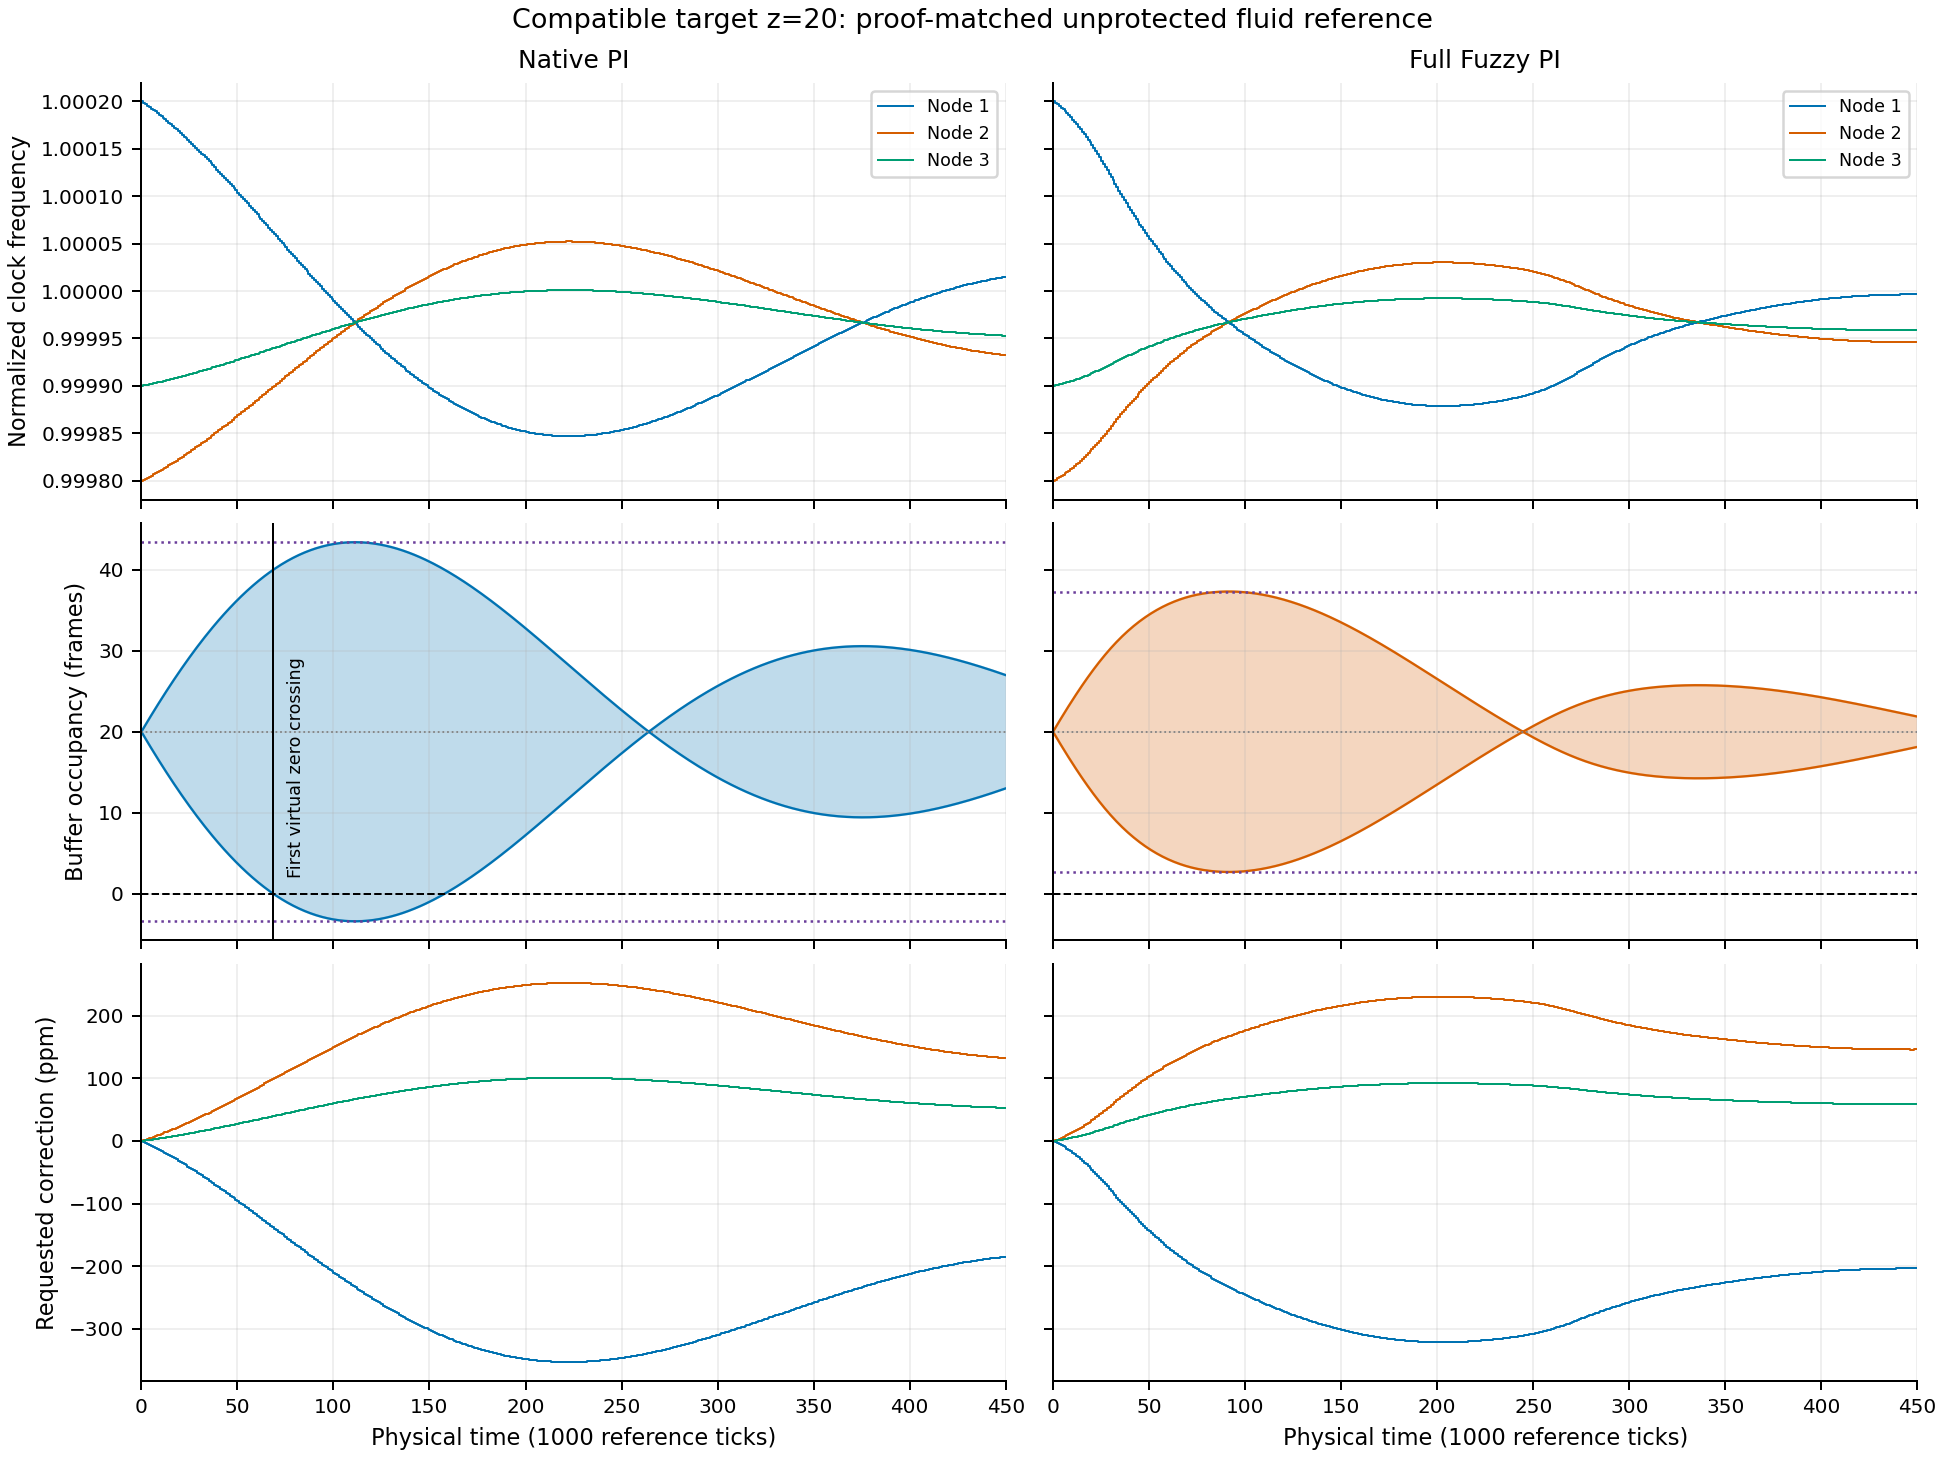
\includegraphics[width=0.94\textwidth]{images/safety_validation_20261105/reference_z20.png}
 \caption{Proof-matched continuous fluid reference at $z=20$ and 400-ppm
 initial spread. Occupancy bands cover all six channels. Fuzzy remains
 above zero, while the unprotected PI trajectory crosses the lower
 boundary. Dotted bounds come from the separate all-time certificate.
 Applied physical frequencies stay positive; signed corrections may be negative.}
 \Description{Matched PI and Fuzzy clock frequencies, fluid buffer envelopes and correction transients.}
 \label{fig:safety_reference_z20}
\end{figure*}

The mismatch grid is
$s\in\{0.25,\allowbreak0.5,\allowbreak0.75,\allowbreak0.85,\allowbreak0.86,\allowbreak1,\allowbreak1.125,\allowbreak1.25,\allowbreak1.5,\allowbreak2\}$.
Figure~\ref{fig:safety_domain} separates the joint sufficient inner
domain from finite-horizon observations at the frozen grid points.
At $z=20$, PI excursions of 19.893146 and 20.127183 frames at
$s=0.85$ and 0.86 bracket its proved directional capacity threshold.
The Fuzzy excursions are computed directly, not scaled linearly.
Successful sampled points do not certify the regions between them;
failure of a sufficient test is recorded as uncertified.

\begin{figure*}[t]
 \centering
 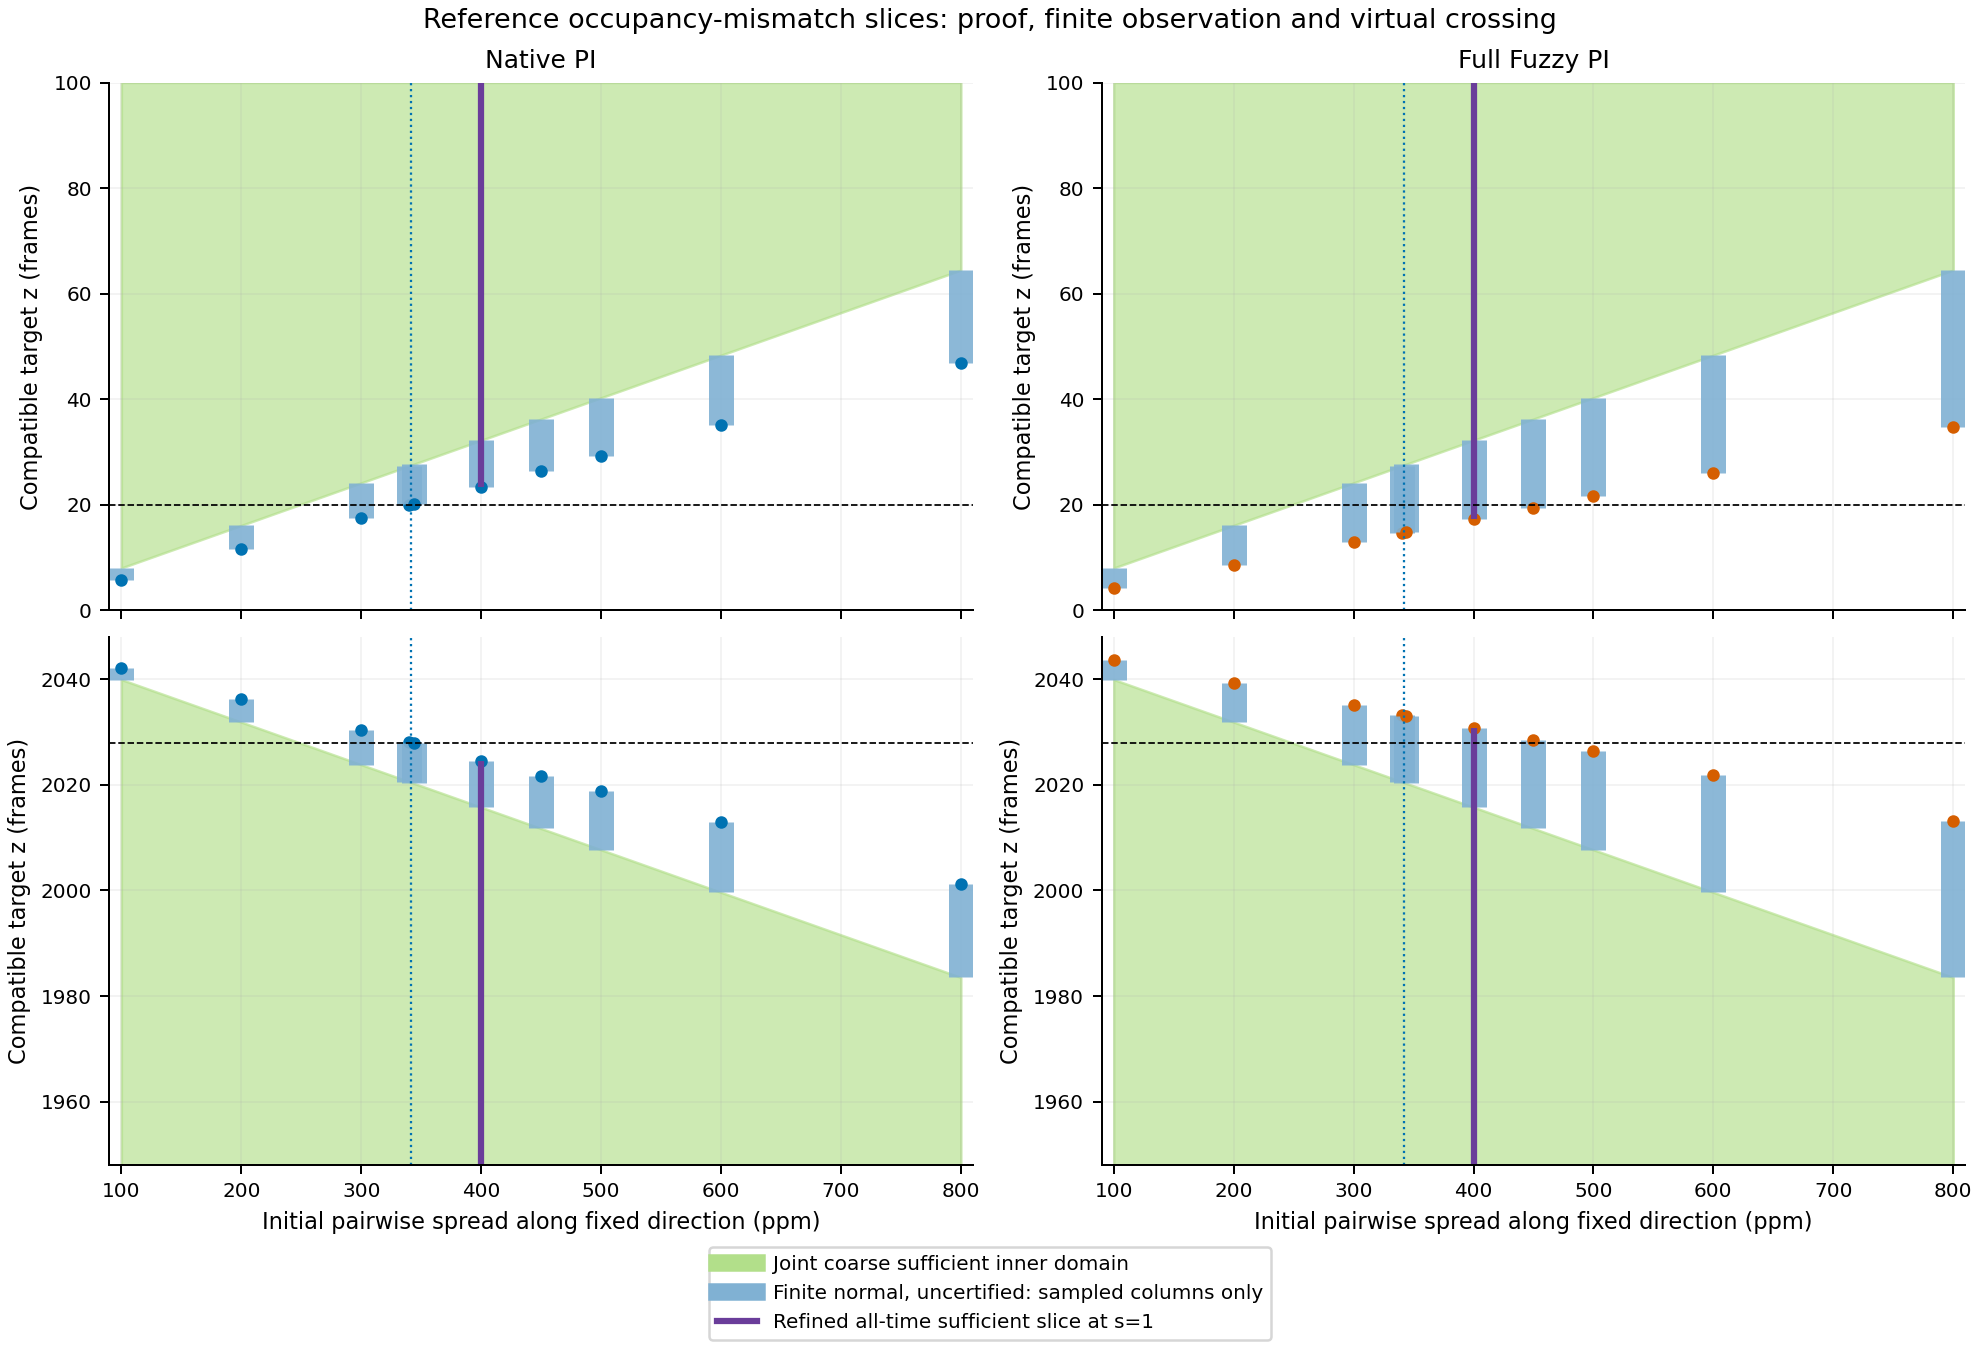
\includegraphics[width=0.94\textwidth]{images/safety_validation_20261105/occupancy_mismatch_domain.png}
 \caption{Compatible-target--mismatch slices at fixed capacity and gains.
 Green denotes the joint coarse sufficient domain. Blue columns extend
 to finite-horizon normal observations at sampled spreads only; markers
 give observed excursion boundaries. Purple denotes the sharper all-time
 slice at $s=1$. The dotted line is PI's directional threshold at $z=20$.
 Central targets are omitted for readability. No untested interpolation
 or delayed-Callisto safety boundary is asserted.}
 \Description{Reference safe configuration slices separating sufficient certificates from sampled trajectory evidence.}
 \label{fig:safety_domain}
\end{figure*}

For the uniform annex, an independent recomputation checks every
one of the 20 parameter cells and reproduces the all-time bound
below 17.342 over 399.6--400.4 ppm. Four direct endpoint runs
are consistent: Fuzzy minima are 2.703366 and 2.668520, whereas
PI minima are $-3.380298$ and $-3.427105$. Their role is to check
the implementation and endpoints; full cell coverage and the
contracting tail supply the uniform theorem.

Two additional zero-mean frequency directions complete the
distribution check. Together with the prescribed direction, all
have 400-ppm spread but $Q=(216,234,288)/30000^2$. Each satisfies
the exact $V_1=H^2c_PQ$ relation. Their Fuzzy peaks differ
(approximately 17.311137, 17.314057 and 17.322842 frames), while
PI peaks coincide for these triangle cases. The energy relation
is a sufficient-domain tool, not an exact-peak ordering rule.

\subsection{Delayed Callisto: normal operation versus protection}
The actual startup cases fix $s=4$, or 1600-ppm initial spread, and
$z\in\{64,83,104,1944,1965,1984\}$. These assess whether the
margin mechanism persists with local timing and integer frames;
they do not apply the reference's numerical boundary to a different
execution model. The low-target cases produce the predicted
qualitative separation (Table~\ref{tab:safety_actual_lower}). At
$z=83$, Fuzzy stays in $[11,155]$ without intervention, while PI
reaches zero and invokes five input-empty guard episodes. The first
occurs at about $71844.672$ physical ticks; summed blocked time is
61.0114 node-ticks. Figure~\ref{fig:safety_actual_z83} distinguishes
physical clock motion from guarded data progress. At $z=64$ both
methods need protection; at $z=104$ both remain normal.

\begin{table}[t]
 \caption{Actual low-target startup at matched gains. Ranges include
 every integer event; guard counts are off episodes, not off/on transitions.}
 \label{tab:safety_actual_lower}
 \centering
 \begin{tabular}{@{}rllll@{}}\toprule
 & \multicolumn{2}{c}{Buffer occupancy / frames} & \multicolumn{2}{c}{Guard episodes}\\
 $z$ & PI & Fuzzy & PI & Fuzzy\\\midrule
 64 & 0--128 & 0--128 & 26 & 6\\
 83 & 0--166 & 11--155 & 5 & 0\\
 104 & 10--198 & 32--176 & 0 & 0\\\bottomrule
 \end{tabular}
\end{table}

\begin{figure*}[t]
 \centering
 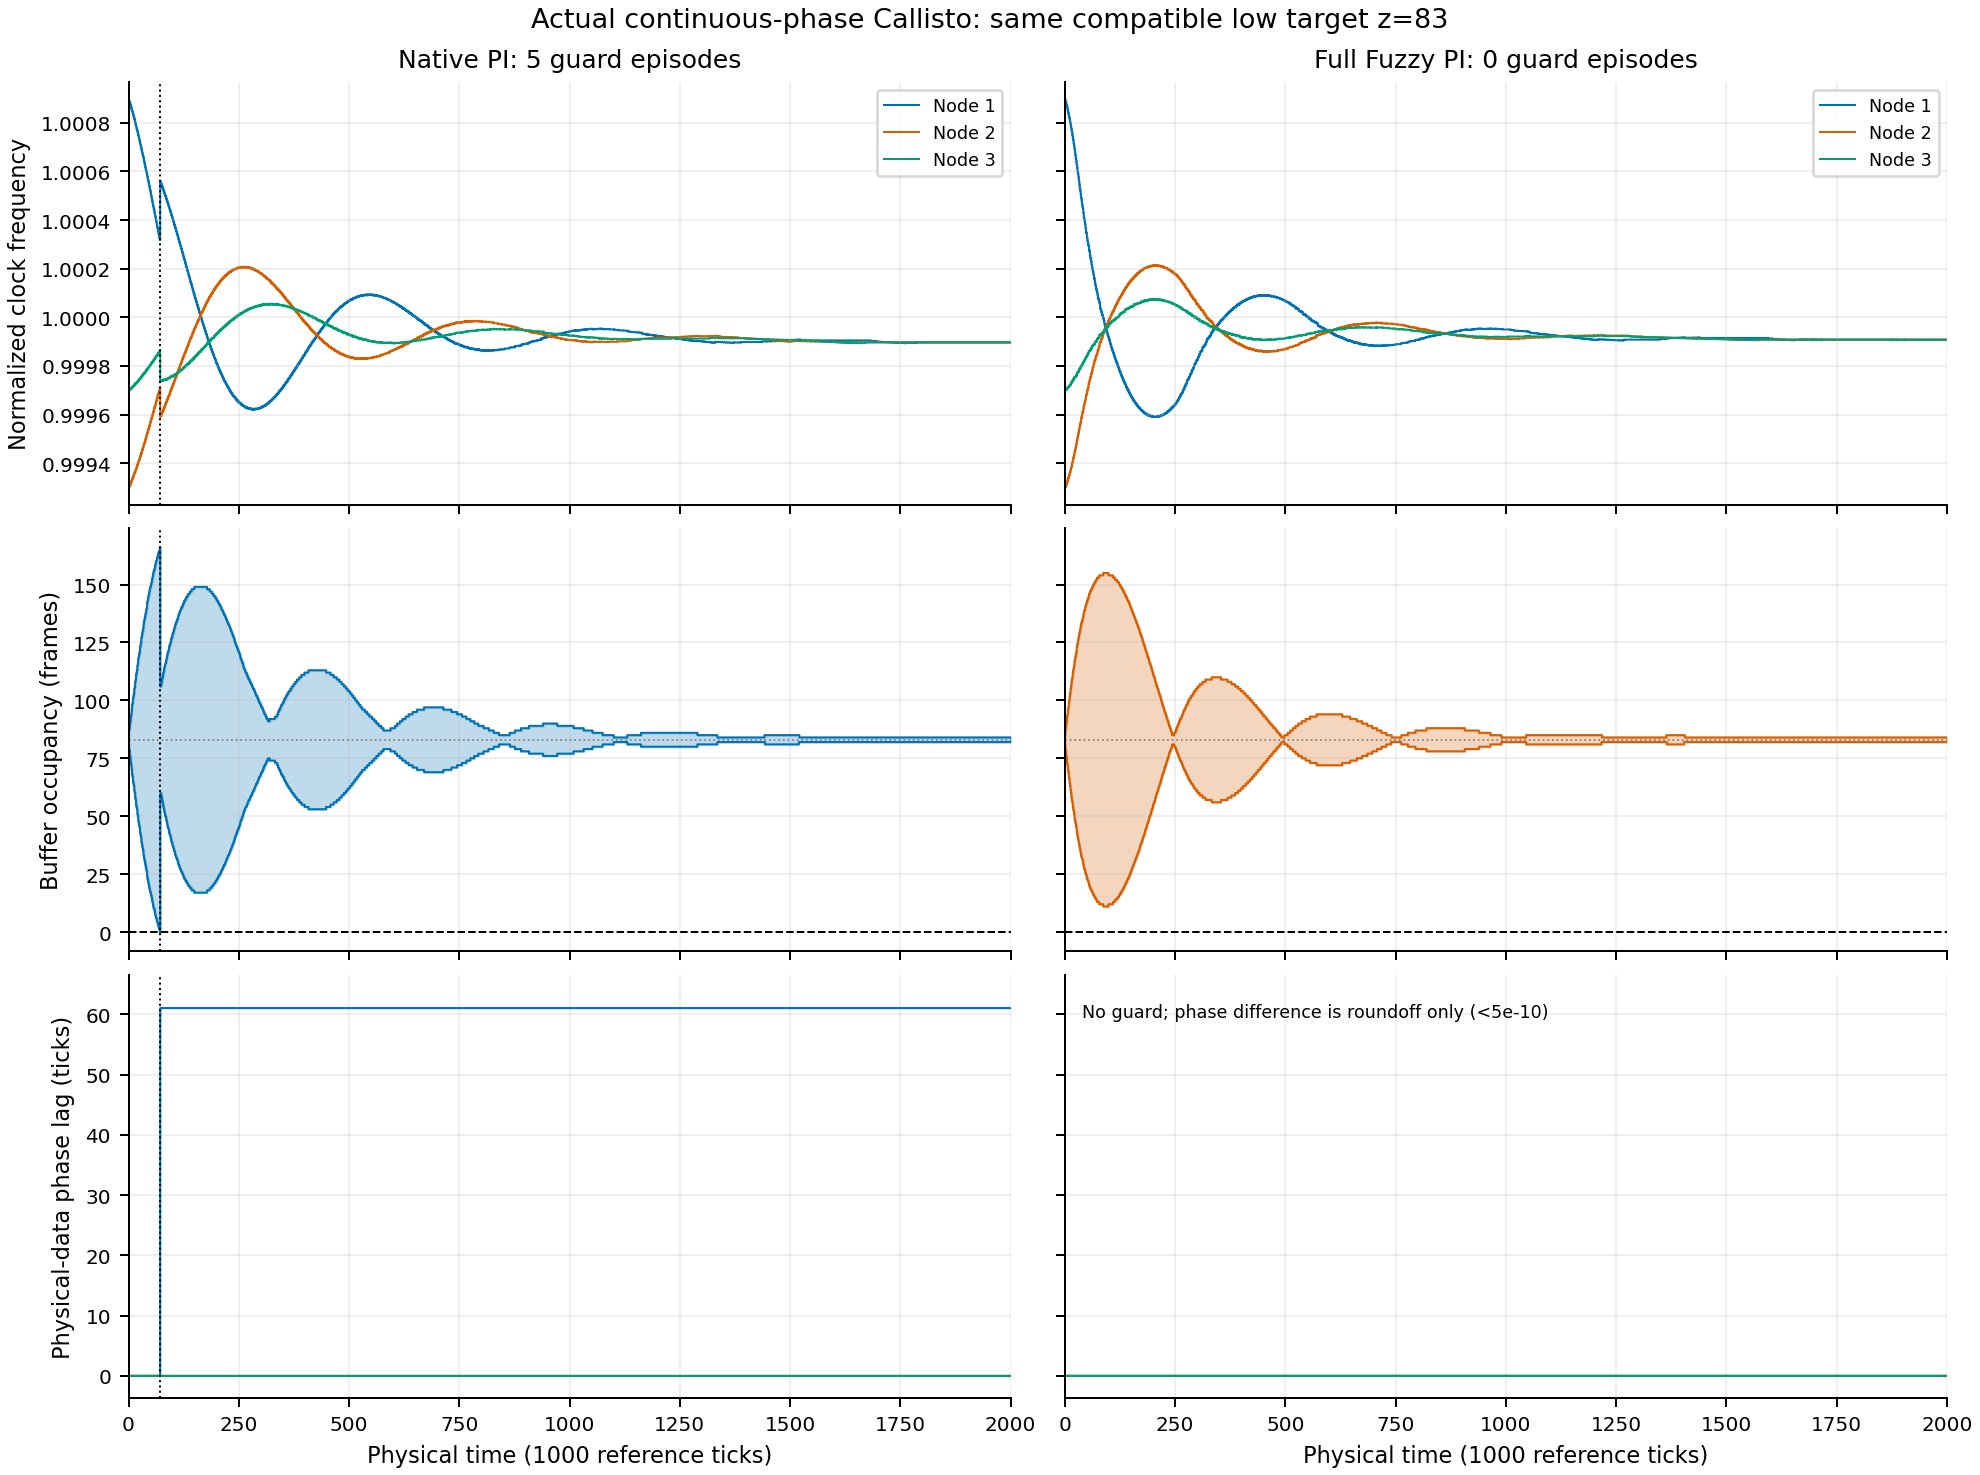
\includegraphics[width=0.94\textwidth]{images/safety_validation_20261105/actual_z83.png}
 \caption{Continuous-phase Callisto at $z=83$, 1600-ppm spread and matched
 gains. Full-event occupancy envelopes show PI reaching zero and Fuzzy
 retaining positive reserve. The dotted line marks PI's first guard.
 Physical-minus-data phase reveals guard-induced progress loss; both
 columns use common axis ranges. This finite delayed execution supports
 the mechanism and is separate from the zero-delay all-time proof.}
 \Description{Actual clock frequencies, buffer occupancies and physical-to-data phase lag for PI and Fuzzy.}
 \label{fig:safety_actual_z83}
\end{figure*}

The upper-target results expose an additional configuration
constraint. All six upper-target runs invoke outgoing-credit
guards even though their maximum receiving occupancy is 2008,
below $C=2048$. Readiness counts source sends minus causally
delayed reverse pops, together with the UGN offset. In this
configuration initial used credit is $z+40$, including both
forward in-flight frames and delayed reverse consumption knowledge.
Thus a simple physical-occupancy mirror of the zero-delay result
does not predict guard-free delayed execution. This configuration-
specific 40-frame observation is not a general latency margin.

All 12 runs retain inclusive physical capacity compliance and
positive clock frequency (minimum 0.9993), without correction
saturation. Nine cases rely on guards. Complete crossing replay
has zero occupancy mismatches, and independent command
reconstruction has maximum residual $1.09\times10^{-19}$.
Pre-first-guard command and measurement prefixes match the old
high-reserve trajectory exactly; all post-guard evolution is newly
run. Fewer guard episodes alone does not prove higher throughput:
at $z=1965$ Fuzzy has fewer episodes but lower final data progress.
Appendix~\ref{app:safety_validation} retains every case, credit
diagnostics and the complete validation protocol.

\subsection{Supplementary disturbance-performance evidence}
Earlier independent tuning and random/burst campaigns answer a
different question. Their complete protocols and results, including
operating limits, are retained in Appendix~\ref{app:evaluation}.
They are not rerun or used as evidence for the safety-domain theorem.
The present evidence chain is the mathematical configuration test,
strict reference comparison and qualitative implementation checks.

\section{Discussion}
\label{sec:discussion}

The analysis links a bittide storage requirement to an initial
frequency mismatch through a specified controller and execution
model. Mismatch energy $\delta\omega^\top L\delta\omega$ captures
how frequency differences are distributed over the graph, while
target placement determines the available lower and upper reserve.
Sampling, gains, normalization and graph resistance enter the same
joint test. These are coupled sufficient conditions; a failed test
does not make a configuration unsafe, and maximum frequency spread
alone does not specify the required reserve.

The Fuzzy advantage has two distinct mathematical components.
The exact nonlinear map explains state-dependent increment shaping;
it does not itself order closed-loop performance. The outward
prefix and contracting tail establish the strict excursion ordering.
At fixed capacity the translation lemma then converts this ordering
into a larger admissible target interval for a prescribed frequency
initialization. Full parameter-cell coverage extends the result to
a narrow, quantified interval along the same mismatch direction.
This is a proved configuration-slice advantage at matched gains,
with positive physical frequencies and no limiter intervention.
It is not a claim that the coarser Lyapunov inner domain is larger
for Fuzzy or that every 400-ppm initialization benefits.

The qualitative experiments directly check these deductions. Their
cases are intentionally chosen around theoretical boundaries and
are not independent statistical discovery. The reference uses the
same continuous held flow as the proof. Callisto separately retains
local scheduling, delay and integer events, so its normal-versus-guard
separation supports the mechanism without transferring the reference
boundary. The upper-target runs identify why receiving occupancy
alone is insufficient for delayed readiness: in-flight data and
reverse-credit delay also consume storage authorization. A physical
buffer below capacity can therefore coexist with a necessary guard.
Fewer guard episodes can accompany lower final data progress.

The occupancy-translation family changes initial occupancy, target
and compatible marking together. It does not certify arbitrary
initial buffer error at a fixed half-capacity target, or preserve
the original application's marking across configurations. Within
each comparison the two controllers have the same marking and
logical configuration. Keeping capacity fixed also preserves
percentage normalization; changing capacity or topology requires
consistent remapping and a fresh certificate.

The nominal reference proves target convergence and syntony with
positive physical progress. Persistent delivery disturbances instead
require finite-window performance measures. Earlier independently
tuned experiments, retained in Appendix~\ref{app:evaluation}, show
benefits in two random regimes and costs in other regimes. They
answer a separate tuning/performance question and do not enlarge
the proved safe domain. Application-level logical synchrony also
requires the prescribed frame relationships; buffer compliance and
frequency agreement do not replace a payload refinement proof.
Extending the invariant analysis to asynchronous sampling, nonzero
link/control delay, integer counts and delayed credit is required
before claiming all-time safety for the full Callisto implementation.


\section{Conclusion}
\label{sec:conclusion}

We proposed an incremental Fuzzy PI controller for bittide and
derived configuration-dependent conditions connecting initial
frequency mismatch, buffer reserve, graph structure and controller
scales. Implementation-consistent PI calibration and the exact
nonlinear rule map make the comparison explicit. For the stated
synchronous zero-delay fluid reference, invariant-domain and
Lyapunov analysis establish convergence, positive physical
frequencies and correction bounds. A certified prefix and infinite
tail prove a smaller Fuzzy buffer excursion and, at fixed capacity,
a strictly larger interval of compatible safe occupancy targets for
the prescribed initialization. Complete interval coverage additionally
certifies a fixed-direction 399.6--400.4-ppm configuration region
where Fuzzy is safe at target 20 while unprotected PI crosses zero.

Theory-directed simulations agree with these reference predictions.
Twelve continuous-phase Callisto runs separately assess delayed
integer execution. At target 83 and 1600-ppm initial spread, Fuzzy
remains in $[11,155]$ without protection, while PI reaches zero and
invokes five input-empty guard episodes. Upper-target cases expose
the additional delayed-credit condition and delimit the reference
mirror argument. The result is a conditional mathematical safety
advantage supported by qualitative implementation evidence, with
all-time claims restricted to the declared reference. Incorporating
asynchronous timing, delay, quantization and credit into a full
execution certificate remains necessary for broader guarantees.


% Funding/acknowledgments remain pending; original placeholder is backed up.


% Main text ends here; keep References and appendices outside the ten-page body.
\clearpage
\label{page:references_start}
\bibliographystyle{ACM-Reference-Format}
\bibliography{references}

\clearpage
\appendix
\begingroup
\setlength{\emergencystretch}{1em}
% Expanded Background, 2026-11-03. Source-only revision; no PDF build.
\section{Extended Background}
\label{app:background}
\noindent\textbf{Correspondence: Section~\ref{sec:background}.} This appendix preserves the extended model, intermediate steps and supporting interpretation behind the corresponding main-text section.


\label{detail:sec:background}

\subsection{Logical Synchrony and the bittide Mechanism}

Logical synchrony describes relationships between distributed events without requiring a global physical clock. In bittide, neighboring nodes exchange ordered frames, and elastic receiving buffers accommodate differences in their physical progress. The association between sending and receiving events provides the basis for a logical execution whose dependencies can be reasoned about independently of exact wall-clock timing. Equal physical phases are therefore not required for logical synchrony. Frequency agreement alone, however, does not establish the required event relationships: frame ordering, initialization and continued availability of the corresponding frames also matter. These distinctions follow the logical-synchrony and multiclock-network framework developed by Lall et al.~\cite{lall2024logicalSynchrony}.

The control problem supports this realization by regulating physical progress while retaining the prescribed frame relationships. Each node observes its own receiving buffers and adjusts its local clock frequency. Buffers consequently provide both the local feedback signal and finite storage for a temporary imbalance between delivery and consumption.

\subsection{Continuous Clocks and Receiving-Buffer Dynamics}

We consider a network of $n$ nodes. Node $i$ has continuous clock phase $\theta_i(t)$, measured in local cycles, and physical frequency

\begin{equation}
\dot\theta_i(t)=\omega_i(t)=\omega_i^u+u_i(t),
\end{equation}

where $\omega_i^u$ is its constant uncontrolled frequency and $u_i(t)$ is the applied frequency correction. The correction can be signed; admissible physical operation requires $\omega_i(t)>0$. In the current Callisto model, corrections are held between local actuation events. Phase remains continuous when a correction changes, although its slope can change. Local sampling and integer frame events are embedded in this continuous-time plant.

For a receiving edge $e=(j\to i)$, let $\beta_e(t)$ be buffer occupancy in frames and $C_e$ its capacity. During normal operation without progress blocking,

\begin{align}
\beta_e(t)&=\beta_e(0)+A_{ji}^{\mathrm{arr}}(t)-N_i(t),\nonumber\\
N_i(t)&=\lfloor\theta_i(t)\rfloor-\lfloor\theta_i(0)\rfloor.
\label{detail:eq:bg_count_balance}
\end{align}

Here $A_{ji}^{\mathrm{arr}}(t)$ counts arrivals during $(0,t]$, including frames already in flight at initialization, and $N_i(t)$ counts local consumption. This conservation relation explains why both clock frequency mismatch and delivery changes affect occupancy. Section~\ref{detail:sec:fpi_controller} specifies the local schedules, initialization and ordered arrival model used in our realization.

Fluid models replace integer frame counts by continuous phase increments. With constant physical link latency $\tau_{ji}$, the corresponding occupancy satisfies, between command discontinuities,

\begin{equation}
\dot{\widetilde\beta}_{ji}(t)
=\omega_j(t-\tau_{ji})-\omega_i(t),
\end{equation}

where $\widetilde\beta_{ji}$ denotes fluid occupancy. Thus occupancy integrates the imbalance between delayed source progress and local consumption. The fluid approximation facilitates analysis; its assumptions must be distinguished from those of integer-frame execution. This separation is also central to existing PI performance analysis~\cite{lall2022resistance} and buffer-occupancy modeling~\cite{lall2024bufferOccupancy}.

\subsection{Safety, Syntony and Buffer Centering}

Safety is a property of the complete trajectory. For the normal operating regime studied here, we seek

\begin{equation}
0<\beta_e(t)<C_e,\qquad
\omega_i(t)>0,\qquad |u_i(t)|\le u_{\max},
\end{equation}

for every edge, node and time, where $u_{\max}>0$ is the correction limit. The available lower and upper buffer reserves are $\beta_e(t)$ and $C_e-\beta_e(t)$, respectively. A convergent trajectory can still exhaust either reserve before reaching its limit. Avoiding such exhaustion through control is distinct from invoking a protection mechanism that blocks logical progress.

Define the physical frequency spread as

\begin{equation}
\Delta_\omega(t)=\max_i\omega_i(t)-\min_i\omega_i(t).
\end{equation}

For nominal fluid operation with fixed conditions, we seek $\Delta_\omega(t)\to0$, together with $\beta_e(t)\to\beta_e^*$ for compatible occupancy targets $\beta_e^*$. Frequency agreement is the nominal syntonization objective; it does not imply zero phase differences or tracking an externally prescribed frequency. Without an external reference, the common limiting frequency $\omega_\infty$ is determined by the closed loop. Likewise, arbitrary per-edge targets cannot be assumed compatible with a fixed marking, meaning the frame-count offsets determined by initialization, and with the selected initial state.

If a transient frequency-spread tolerance $\Delta_{\mathrm{safe}}>0$ is specified, then $\Delta_\omega(t)<\Delta_{\mathrm{safe}}$ is an additional engineering constraint. It is not the definition of logical synchrony. Under persistent delivery perturbations, we assess bounded deviations, residual disagreement and buffer reserves rather than assume exact disturbance-free centering.

\subsection{Delivery Perturbations and Local Feedback}

A latency increase affects the delivery process before a receiver necessarily observes it through its next control measurement. If arrivals pause while consumption continues, the conservation relation shows that the receiving buffer decreases; subsequent release of accumulated frames can instead increase occupancy. The disturbance therefore acts through frame availability and accumulated count imbalance. A controller cannot recreate an undelivered frame, and its response is constrained by measurement and actuation timing. Our experiments use declared order-preserving delivery traces so that controller comparisons share the same external stress definition. The exact arrival construction is given in Section~\ref{detail:sec:fpi_controller}.

\subsection{Existing Control Foundations and the Present Study}

Existing work analyzes occupancy-feedback PI performance through controller gains and graph resistance distances, derives limiting fluid occupancies, and develops reframing methods that separate frequency regulation from occupancy positioning. These are complementary foundations: PI performance~\cite{lall2022resistance}, steady buffer occupancy~\cite{lall2024bufferOccupancy}, and buffer centering~\cite{lall2023bufferCentering}. Their conclusions apply under their respective modeling assumptions; in particular, continuous-time gain conditions cannot be transferred unchanged to sampled execution with delay.

This paper builds on those foundations by proposing a local incremental Fuzzy PI law and analyzing how its nonlinear increments reshape the closed-loop response at explicitly calibrated PI scales. Section~\ref{detail:sec:fpi_controller} defines the complete controller and establishes that calibration. Section~\ref{detail:sec:btd_reference} derives sufficient safety and convergence conditions for a declared synchronous, zero-latency fluid reference, followed by an all-time buffer-excursion comparison for one prescribed initialization. Evaluation in continuous-phase Callisto separately examines delivery perturbations under the actual local update and frame-count conventions.

% Expanded, input-ready Section III. No standalone preamble or PDF build.
\section{Controller Realization and Complete Derivations}
\label{app:controller}
\noindent\textbf{Correspondence: Section~\ref{sec:fpi_controller}.} This appendix preserves the extended model, intermediate steps and supporting interpretation behind the corresponding main-text section.


\label{detail:sec:fpi_controller}
We propose a decentralized, occupancy-based incremental Fuzzy PI controller
for bittide. Each node combines receiving-buffer error with its
update-to-update change to compute an frequency correction increment.
This section specifies the complete controller and its continuous-clock
interface, derives an implementation-consistent PI calibration, and
establishes the nonlinear properties used in
Section~\ref{detail:sec:btd_reference}. The physical plant, integer frame counts
and sampled controller state are kept distinct throughout the derivation.

\subsection{Continuous-clock realization of the proposed controller}

\label{detail:subsec:fpi_laws}
The plant is the current continuous-phase Callisto model within the bittide
framework~\cite{lall2024logicalSynchrony}. For constant
uncontrolled clock frequency $\omega_i^u$ and applied correction $u_i(t)$,
\begin{align}
 \dot\theta_i(t)&=\omega_i^u+u_i(t),\nonumber\\
 u_i(t)&=u_{i,k},\qquad t\in[t^a_{i,k},t^a_{i,k+1}),\nonumber\\
 \theta_i(t)&=\theta_i(t^a_{i,k})+
       (\omega_i^u+u_{i,k})(t-t^a_{i,k}).
 \label{detail:eq:fpi_continuous_plant}
\end{align}
The superscript $a$ denotes actuation, and $k$ indexes that node's updates.
Normal executions require $\omega_i^u+u_i(t)>0$, so the phase has a
monotone inverse. Physical phase is continuous at an update; its slope can change. Requested
correction $q_{i,k}$ is computed from the measured buffers and applied as
$u_{i,k}=\operatorname{sat}_{u_{\max}}(q_{i,k})$, with
$\operatorname{sat}_b(z)=\min\{b,\max\{-b,z\}\}$ and $u_{\max}>0$.
The proposed controller has jump updates inside a continuous physical plant;
it is not implemented as an ordinary differential equation for its accumulator.

Let $p>0$ be the polling period and $d_{\rm ctrl}\ge0$ the execution delay,
both measured in local-clock phase units. Measurement time $t^m_{i,k}$
and actuation time $t^a_{i,k}$ satisfy
\begin{align}
 \theta_i(t^m_{i,k})&=\theta_i(0)+k\,p,\nonumber\\
 \theta_i(t^a_{i,k})&=\theta_i(0)+k\,p+d_{\rm ctrl},\nonumber\\
 \int_{t^m_{i,k}}^{t^a_{i,k}}(\omega_i^u+u_i(s))\,ds&=d_{\rm ctrl}.
 \label{detail:eq:fpi_local_schedule}
\end{align}
The product $k\,p$ in these scheduling equations means the integer index
$k$ multiplied by the poll period $p$; it is not the proportional gain
$k_p$. With zero initial correction, $t^m_{i,0}=0$ and
$t^a_{i,0}=d_{\rm ctrl}/\omega_i^u$. Subsequent actuation intervals equal
$p/(\omega_i^u+u_{i,k})$. The delay is not automatically a constant
physical time, and its age must not be computed using the new command
that is applied only at the end of that age interval.

In normal operation, each integer source-phase crossing sends a frame.
With the progress guards open, frame conservation gives
\begin{equation}
 \beta_{j\to i}(t)=\beta_{j\to i}(0)+A^{\rm arr}_{ji}(t)-N_i(t),
 \label{detail:eq:fpi_count_balance}
\end{equation}
where $A^{\rm arr}_{ji}(t)$ counts arrivals during $(0,t]$, including
initial in-flight frames, and
$N_i(t)=\lfloor\theta_i(t)\rfloor-\lfloor\theta_i(0)\rfloor$ counts
local consumption. For a constant physical delay $\tau_{ji}\ge0$,
\begin{equation}
 A^{\rm arr}_{ji}(t)=\lfloor\theta_j(t-\tau_{ji})\rfloor
                  -\lfloor\theta_j(-\tau_{ji})\rfloor.
 \label{detail:eq:fpi_fixed_delay_arrivals}
\end{equation}
Thus arrival counts incorporate the declared negative-time history.

For constant physical link latency $\tau_{ji}$, receiving occupancy is
\begin{equation}
 \beta_{j\to i}(t)=\lambda^{\rm UGN}_{ji}
 +\lfloor\theta_j(t-\tau_{ji})\rfloor-\lfloor\theta_i(t)\rfloor.
 \label{detail:eq:fpd_continuous_fifo}
\end{equation}
Here $\lambda^{\rm UGN}_{ji}$ is the fixed integer offset in the absolute
phase-count convention. It is determined by occupancy and prehistory:
\begin{equation}
 \lambda^{\rm UGN}_{ji}=\beta_{j\to i}(0)
 -\lfloor\theta_j(-\tau_{ji})\rfloor+\lfloor\theta_i(0)\rfloor.
 \label{detail:eq:fpd_ugn_init}
\end{equation}
The relative-count logical marking is
$\lambda^{\rm LSN}_{ji}=\lambda^{\rm UGN}_{ji}
+\lfloor\theta_j(0)\rfloor-\lfloor\theta_i(0)\rfloor$;
the two coincide when the initial phase counts are equal.

For changing delivery times, let $s_{j,m}=\theta_j^{-1}(m)$ be the send
time of source tick $m$, and $a_{ji}(s)$ its causal ordered arrival map.
For the desired send-time delay profile $\tau_{ji}(s)$, the declared
running-maximum envelope is
\[
 a_{ji}(s)=\sup_{r\le s}\{r+\tau_{ji}(r)\},
\]
including the constant-delay negative-time history.
Define the delivered tick frontier
\begin{equation}
 \begin{aligned}
 C^{\rm arr}_{ji}(t)&=\max\{m\in\mathbb Z:a_{ji}(s_{j,m})\le t\},\\
 \beta_{j\to i}(t)&=\lambda^{\rm UGN}_{ji}
       +C^{\rm arr}_{ji}(t)-\lfloor\theta_i(t)\rfloor.
 \end{aligned}
 \label{detail:eq:fpd_ordered_arrivals}
\end{equation}
The negative-time history specifies initial in-flight frames. The declared
running-maximum arrival envelope preserves order and can release a batch
after a desired-delay decrease; it imposes no finite serialization rate.
At an upward-delay discontinuity, a supremum of continuous source times
need not itself have arrived. Counting delivered tick indices avoids
silently including such a boundary frame.

If a protection guard blocks logical progress, the runtime can retain a
separate continuous data phase $\psi_i$ with
$\dot\psi_i=g_i(t)\dot\theta_i$, where $g_i\in\{0,1\}$ is the progress
gate. Buffer counts then use $\psi_i$, whereas scheduling still uses
$\theta_i$. In the ungated normal regime, with matching initial phases, data phase and physical phase agree. Guard operation does not stop the oscillator.

Only for the reference proof do we replace integer occupancy by a
fluid counterpart. At constant delay, define
$\widetilde\beta_{ji}(t)=\widetilde\lambda_{ji}
+\theta_j(t-\tau_{ji})-\theta_i(t)$, where
$\widetilde\lambda_{ji}$ is an additive offset chosen for the specified
fluid initialization. Between command discontinuities,
\begin{equation}
 \dot{\widetilde\beta}_{ji}(t)
 =\omega_j^u+u_j(t-\tau_{ji})-\omega_i^u-u_i(t).
 \label{detail:eq:fpi_fluid_counterpart}
\end{equation}
This derivative belongs to the fluid counterpart, not the actual integer
occupancy. Replacing floor counts by phases does not automatically preserve
an arbitrary initialization; the compatible zero-latency marking used in
Section~\ref{detail:sec:btd_reference} is specified there.

\subsection{Notation and the measured error}

Node $i$ has incoming-neighbor set $\mathcal N_i^-$ and $d_i=|\mathcal N_i^-|>0$ incoming channels. All incoming sums below range over $j\in\mathcal N_i^-$. This section assumes fixed active
incoming sets: the runtime link-status mask is one on all configured inputs.
The Fuzzy percentage wrapper averages its configured inputs, so changing
link masks would require an explicit corresponding measurement policy.
At the $k$th local measurement,
$\beta_{ji,k}$ is the measured occupancy of channel $j\to i$, and
$\beta^*_{ji}$ is its fixed target. Use
\begin{equation}
 E_{i,k}=\sum_{j\in\mathcal N_i^-}(\beta_{ji,k}-\beta^*_{ji}).
 \label{detail:eq:fpi_error}
\end{equation}
The sign is actual minus target. If incoming buffers are too full, a
positive frequency correction increases local consumption. This explains
the positive PI gains with this error convention. The physical frequency is $\omega_i=\omega_i^u+u_i$, where $\omega_i^u$ is the constant uncontrolled frequency; $u_i$ is a correction, not the entire frequency.

\begin{center}
\begin{tabular}{@{}ll@{}}
\toprule
Symbol & Meaning \\
\midrule
$E_{i,k}$ & Sum error in frames \\
$e_{i,k}$ & Target-minus-measured error in percentage points \\
$I_{i,k}$ & PI baseline sum of sampled frame errors \\
$A_{i,k}$ & Fuzzy accumulator: total requested correction \\
$q_{i,k},u_{i,k}$ & Requested and applied frequency corrections \\
$h$ & Fixed PI baseline integration scale \\
$X_{i,k},Y_{i,k}$ & Scaled Fuzzy error and sample-difference inputs \\
$F_0,\mathcal R_F$ & Linear counterpart and residual $F-F_0$ \\
\bottomrule
\end{tabular}
\end{center}

The event index $k$ is local to a node. The normalization factor $\gamma_i$ converts a frame-sum error into percentage points. The maximum correction $u_{\max}>0$ is the actuator limit; $q$ and $u$ remain distinct if clipping acts. Two nodes need not measure at the
same physical times. The subscript $ji$ abbreviates edge $j\to i$.
Suppressing $i$ below is a notational convenience, not a synchrony
assumption; in that notation $\gamma=\gamma_i$.

\subsubsection{Deriving the percentage-to-frame-error relation}
For common incoming capacity $C$, define
\[
 \bar p_{i,k}=\frac1{d_i}\sum_j\frac{100\beta_{ji,k}}{C},\qquad
 r_i=\frac1{d_i}\sum_j\frac{100\beta^*_{ji}}{C}.
\]
Then subtraction and factoring give
\begin{align}
 e_{i,k}&=r_i-\bar p_{i,k}\\
 &=-\frac{100}{d_iC}\sum_j(\beta_{ji,k}-\beta^*_{ji})
 =-\gamma_i E_{i,k},\qquad \gamma_i=\frac{100}{d_iC}.
 \label{detail:eq:fpi_percent}
\end{align}
For midpoint targets this is the original absolute-percentage input with
$r_i=50$. For other targets the runtime can supply a centered percentage
$r_i+d_i^{-1}\sum_j100(\beta_{ji,k}-\beta^*_{ji})/C$; subtracting it from
$r_i$ yields the same $e_{i,k}$. A mismatched setpoint instead adds a
constant bias and invalidates the scalar relation used for calibration.

With unequal capacities and a consistently matched target reference, the
percentage average gives
\[
 e_{i,k}=-\frac{100}{d_i}\sum_j
 \frac{\beta_{ji,k}-\beta^*_{ji}}{C_{ji}}.
\]
This is a weighted error and generally cannot be written as one normalization constant
times the unweighted PI error sum. Matching such a controller requires a
consistent measurement weighting or a different baseline.

\subsection{PI baseline: update order, units and the first call}

The occupancy-feedback PI baseline is grounded in the bittide analysis
of~\cite{lall2022resistance}. The implemented PI update is an
integrate-then-output recursion:
\begin{equation}
 I_k=I_{k-1}+E_k,\qquad
 q_k^{\rm PI}=k_pE_k+\kappa_I I_k,\qquad \kappa_I=k_i h.
 \label{detail:eq:fpi_native}
\end{equation}
The sum $I_k$ contains no physical time multiplier; $h$ is incorporated in
$\kappa_I$. In the present runtime,
\begin{equation}
 h=\frac{p}{\omega_{\rm base}}.
 \label{detail:eq:fpd_h}
\end{equation}
Here $p$ is the local polling period and $\omega_{\rm base}$ is the fixed implementation reference frequency. The scale $h$ stays fixed during the configured run. Local polling intervals measured
in physical time can vary as the local clock frequency changes; replacing $h$ by
those intervals would implement a different PI law.

Subtract the previous requested output:
\begin{align}
 q_k^{\rm PI}-q_{k-1}^{\rm PI}
 &=k_p(E_k-E_{k-1})+\kappa_I(I_k-I_{k-1})\\
 &=k_p(E_k-E_{k-1})+\kappa_I E_k.
 \label{detail:eq:fpi_pi_increment}
\end{align}
This is the correct increment to reproduce. It contains the present
$E_k$ in the integral term because integration precedes output.

At zero initial sum, the first call returns
\begin{equation}
 q_0^{\rm PI}=(k_p+\kappa_I)E_0.
 \label{detail:eq:fpd_first}
\end{equation}
No physical prehistory measurement is needed to express this algebra:
one may use the fictitious previous error $E_{-1}=0$ and previous requested
output $q_{-1}=0$. That bookkeeping choice is separate from deriving a
plant identity such as $x_k-x_{k-1}=H w_{k-1}$, which requires a genuine
elapsed plant interval.

\subsection{The proposed Fuzzy PI controller}

The proposed local incremental control law combines the present error
and its sample difference as follows:
\begin{align}
 X_k&=K_e e_k,&Y_k&=K_{\Delta e}(e_k-e_{k-1}),\\
 A_k&=A_{k-1}+K_uF(X_k,Y_k),&q_k^{\rm F}&=A_k.
 \label{detail:eq:fpi_fuzzy_law}
\end{align}
The gain signs used here are $K_e,K_{\Delta e}>0$ and $K_u<0$. Thus high occupancy
produces negative $e$, and a negative surface output produces a positive
correction increment. The quantity $e_k-e_{k-1}$ is not divided by elapsed
time; calling it a time derivative would obscure its sampling dependence.

\subsubsection{Memberships and rule weights}
The labels NL, NS, ZE, PS and PL mean negative large, negative small, zero, positive small and positive large, respectively. Each membership $\varphi_a(z)\in[0,1]$ is an activation degree; a singleton is a numerical rule consequent. Let $[z]_+=\max\{z,0\}$ and $\operatorname{clip}_{[0,1]}z$
denote projection onto $[0,1]$. The exact memberships can be written
\begin{align}
 \varphi_{\rm NL}(z)&=\operatorname{clip}_{[0,1]}\frac{-z-5}{5},&
 \varphi_{\rm NS}(z)&=[1-|z+5|/5]_+,\nonumber\\
 \varphi_{\rm ZE}(z)&=[1-|z|/5]_+,&
 \varphi_{\rm PS}(z)&=[1-|z-5|/5]_+,\nonumber\\
 \varphi_{\rm PL}(z)&=\operatorname{clip}_{[0,1]}\frac{z-5}{5}.
 \label{detail:eq:fpi_full_memberships}
\end{align}
Table~\ref{detail:tab:fpi_full_rules} gives all 25 consequent rules.
\begin{table}[t]
\caption{Rule consequents of the proposed bittide Fuzzy PI controller.}
\label{detail:tab:fpi_full_rules}
\centering
\begin{tabular}{@{}c|ccccc@{}}
\toprule
$X\backslash Y$ & NL & NS & ZE & PS & PL\\
\midrule
NL & NL & NL & NL & NS & ZE\\
NS & NL & NL & NS & ZE & PS\\
ZE & NL & NS & ZE & PS & PL\\
PS & NS & ZE & PS & PL & PL\\
PL & ZE & PS & PL & PL & PL\\
\bottomrule
\end{tabular}
\end{table}
Order the labels as NL, NS, ZE, PS and PL, with label indices
$a,b\in\{1,\ldots,5\}$. With singleton values
$(s_1,\ldots,s_5)=(-5,-2.5,0,2.5,5)$ and
$\ell(a,b)=\min\{5,\max\{1,a+b-3\}\}$, compute
\begin{equation}
 w_{ab}=\min\{\varphi_a(X),\varphi_b(Y)\},\qquad
 F(X,Y)=\frac{\sum_{a,b}w_{ab}s_{\ell(a,b)}}{\sum_{a,b}w_{ab}}.
 \label{detail:eq:fpi_rules}
\end{equation}
The membership partition gives at least one positive input membership on
each axis, hence a positive denominator at finite inputs. Individual rules
are summed even when they share a consequent. Replacing this accumulation
by maximum aggregation changes the map and its derivation.

The weighted-average property gives $|F|\le5$ and therefore
$|A_k-A_{k-1}|\le5|K_u|$. This is a per-update bound, not a bound on $A_k$
over an arbitrarily long execution. The raw Fuzzy module itself has no
final correction clipping.
Initialize $A_{i,-1}=0$ and $e_{i,-1}=0$. At each measurement, form
$e_{i,k}$ and $(X_{i,k},Y_{i,k})$, evaluate the rule weights and normalized
surface, increment $A_{i,k}$, and store $e_{i,k}$ as the previous error.
The requested correction is then limited and applied at $t^a_{i,k}$, and
held until the next actuation. In the normal-run policy considered here,
external clipping retains the raw accumulator and anti-windup is disabled.
The controller does not overwrite $A_{i,k}$ with the applied command.
The membership functions, rule consequents and gains stay fixed during a
run; the correction changes with the measured input pair. The law requires
neither an observer nor an FFP mode.


\subsection{Exact PI Calibration, Including Initialization}
\label{detail:subsec:fpi_calibration}

Define the globally linear counterpart
\begin{equation}
 F_0(X,Y)=\frac{X+Y}{2}.
 \label{detail:eq:fpi_f0}
\end{equation}
Replacing $F$ by this map retains the same controller accumulator.
Using $e=-\gamma E$ gives
\begin{align}
 A^0_k-A^0_{k-1}
 &=\frac{K_u}{2}\{K_e e_k+K_{\Delta e}(e_k-e_{k-1})\}\\
 &=-\frac{K_u\gamma K_e}{2}E_k
   -\frac{K_u\gamma K_{\Delta e}}2(E_k-E_{k-1}).
 \label{detail:eq:fpi_substitution}
\end{align}
Matching the two independent coefficients in~\eqref{detail:eq:fpi_pi_increment}
yields
\begin{equation}
 k_p=-\frac{K_u\gamma K_{\Delta e}}2,\qquad
 \kappa_I=-\frac{K_u\gamma K_e}2.
 \label{detail:eq:fpi_matching}
\end{equation}
Solving for two Fuzzy gains with chosen $K_e>0$ gives
\begin{equation}
 K_u=-\frac{2k_ih}{\gamma K_e},\qquad
 K_{\Delta e}=\frac{K_ek_p}{k_ih}.
 \label{detail:eq:fpi_design_gains}
\end{equation}
The formulas assume $k_i h>0$. Pure proportional control is a separate
limiting case and should not be inserted into this inverse mapping with
a zero denominator.

\begin{btdproposition}[Event-level linear-counterpart equivalence]
\label{detail:prop:fpi_equivalence}
For any measurement sequence, suppose~\eqref{detail:eq:fpi_matching} holds and
initialize
\begin{equation}
 A^0_{-1}=k_pE_{-1}+\kappa_I I_{-1},\qquad e_{-1}=-\gamma E_{-1}.
 \label{detail:eq:fpi_initialization}
\end{equation}
Then
$A^0_k=k_pE_k+\kappa_I I_k$ for every $k\ge0$.
\end{btdproposition}
\begin{proof}
Assume the relation holds before update $k$. Substitution gives
\begin{align*}
 A^0_k
 &=k_pE_{k-1}+\kappa_I I_{k-1}
   +k_p(E_k-E_{k-1})+\kappa_I E_k\\
 &=k_pE_k+\kappa_I(I_{k-1}+E_k)
 =k_pE_k+\kappa_I I_k.
\end{align*}
The stated initialization supplies the induction base, including $k=0$.
\end{proof}

\subsubsection{Why zero constructors work for a nonzero first error}
Take $I_{-1}=A^0_{-1}=e_{-1}=0$, corresponding to $E_{-1}=0$.
The first Fuzzy-reference input is
\[
 (X_0,Y_0)=(-\gamma K_eE_0,-\gamma K_{\Delta e}E_0),
\]
so
$A^0_0=(k_p+\kappa_I)E_0$, exactly as in~\eqref{detail:eq:fpd_first}.
If only Fuzzy is warmed up to $e_{-1}=e_0$ while $A^0_{-1}=0$, its
difference input vanishes and the output is merely $\kappa_I E_0$.
The missing $k_pE_0$ term can create a large apparent controller difference
unrelated to fuzzy inference.

\subsubsection{A numerical calibration from the present configuration}
For $d=2$, $C=2048$, $p=1000$, $\omega_{\rm base}=29999/30000$,
$k_p=2\times10^{-6}$, $k_i=5\times10^{-11}$ and $K_e=0.1$,
\begin{align}
 \gamma&=\frac{25}{1024},&h&=\frac{30000000}{29999},\nonumber\\
 \kappa_I&=\frac3{59998000},&
 K_u&=-\frac{768}{18749375},\nonumber\\
 K_{\Delta e}&=\frac{29999}{7500}
 \simeq3.9998666667.
 \label{detail:eq:fpd_example_gains}
\end{align}
For a one-frame first error, the matched PI and $F_0$ corrections are both
$2.0500016667\times10^{-6}$. Warming up only the Fuzzy previous error
instead gives approximately $5.0001666722\times10^{-8}$. The example
illustrates an initialization mismatch; it is not a new plant simulation.

\subsubsection{Execution-layer conditions}
Identical raw outputs give identical applied outputs under a common
limiter when raw states are retained and anti-windup is disabled.
Tracking or reset requires compatible state changes. For example, after
processing $E_k$, setting
\[
 A^0_k=u_{\rm held},\qquad
 I_k=\frac{u_{\rm held}-k_pE_k}{\kappa_I},\qquad
 e_k=-\gamma E_k
\]
restores the state relation for the next ordinary update. A branch designed
to produce a held output on an immediate extra update requires its own
integrate-first adjustment; the above is not an instruction to add an
extra call. Limiting the internal reference $F_0$ to $[-5,5]$ also changes
the controller, even if the external correction limiter is shared.

Under a deterministic causal plant, the same initial history, measured
inputs, actuation order, external trace and compatible resets imply
closed-loop equality by induction over events. No globally synchronous
physical grid is required for this algebraic equivalence. By contrast,
matching only labels such as ``same gains'' or ``same random seed'' does
not establish these conditions.

\subsection{Deriving the Exact Central Nonlinear Surface}
\label{detail:subsec:fpi_mechanism}

For $0<r\le5$, define
\begin{align}
 \Omega_r&=\{(X,Y):|X|+|Y|\le r\},\nonumber\\
 m&=\min(|X|,|Y|),\qquad s=|X|+|Y|.
 \label{detail:eq:fpi_domain}
\end{align}
The same-sign interaction is
\begin{equation}
 J(X,Y)=\begin{cases}\operatorname{sgn}(X)m,&XY>0,\\0,&XY\le0.\end{cases}
 \label{detail:eq:fpi_interaction}
\end{equation}
For points in $\Omega_5$, put $a=|X|/5$, $b=|Y|/5$.
Because $a+b\le1$, each input has only its central and sign-adjacent
membership active. Their four joint min weights are
\begin{align}
 w_{00}&=\min(1-a,1-b)=1-\max(a,b),\nonumber\\
 w_{s0}&=\min(a,1-b)=a,\nonumber\\
 w_{0s}&=\min(1-a,b)=b,\nonumber\\
 w_{ss}&=\min(a,b).
 \label{detail:eq:fpd_four_weights}
\end{align}
The subscripts $s$ denote the input's active sign label, not the scalar
$s=|X|+|Y|$. Zero-input boundaries follow by continuity.

The denominator is therefore
\begin{equation}
 D=1-\max(a,b)+a+b+\min(a,b)
  =1+2\min(a,b)=1+2m/5.
 \label{detail:eq:fpd_denominator}
\end{equation}
The central-central consequent is zero. The sign-central and
central-sign rules contribute $(5/2)\operatorname{sgn}(X)a=X/2$
and $(5/2)\operatorname{sgn}(Y)b=Y/2$.
For equal signs, the joint consequent is
$5\operatorname{sgn}(X)$ and contributes $\operatorname{sgn}(X)m$;
for opposing signs it is zero. The four quadrants therefore give
\begin{equation}
 F(X,Y)=\begin{cases}
 \dfrac{F_0+m}{1+2m/5},&X>0,\ Y>0,\\[4pt]
 \dfrac{F_0-m}{1+2m/5},&X<0,\ Y<0,\\[4pt]
 \dfrac{F_0}{1+2m/5},&X>0,\ Y<0,\\[4pt]
 \dfrac{F_0}{1+2m/5},&X<0,\ Y>0.
 \end{cases}
 \label{detail:eq:fpi_quadrants}
\end{equation}
On either axis $m=0$, giving $F=F_0$. These cases establish the following
identity, including boundaries by continuity.
\begin{btdproposition}[Exact central surface]
\label{detail:prop:fpi_central}
For every $(X,Y)\in\Omega_5$,

\begin{equation}
 \begin{aligned}
 F(X,Y)&=\frac{(X+Y)/2+J(X,Y)}{1+2m/5},\\
 J(X,Y)&=\begin{cases}\operatorname{sgn}(X)m,&XY>0,\\0,&XY\le0.
 \end{cases}
 \end{aligned}
 \label{detail:eq:fpi_central}
\end{equation}
\end{btdproposition}
This is an exact rule-level identity on $\Omega_5$, not a fitted
approximation. Outside this diamond, the cross weights in
\eqref{detail:eq:fpd_four_weights} need not equal $a$ and $b$, so the formula
must not be extended without a new case analysis.

\subsection{Sign-conditioned response, sector and nonlinear geometry}

\subsubsection{Same-sign enhancement}
When $XY>0$, $F_0$ has magnitude $s/2$ and the same sign as $X$.
Equation~\eqref{detail:eq:fpi_central} gives
\begin{equation}
 \frac{F}{F_0}=\frac{1+2m/s}{1+2m/5}.
 \label{detail:eq:fpi_same_sign}
\end{equation}
Since $s\le5$, its numerator is at least the denominator. Since
$m\le s/2$, the numerator is at most 2. Thus $1\le F/F_0\le2$.
Define the normalized nonlinear residual by
$\mathcal R_F(X,Y)=F(X,Y)-F_0(X,Y)$. Subtracting $F_0$ gives
\begin{equation}
 \mathcal R_F=
 \frac{\operatorname{sgn}(X)m(1-s/5)}{1+2m/5},\qquad XY>0.
 \label{detail:eq:fpd_same_residual}
\end{equation}
For instance, $F(0.1,0.1)=0.2/1.04\simeq0.19230769$, compared with
$F_0=0.1$. Both are surface values; the actual increment multiplies by
negative $K_u$.

\subsubsection{Opposing-sign attenuation and zero-output cases}
When $XY<0$, the interaction vanishes, so
\begin{equation}
 F=\frac{F_0}{1+2m/5},\qquad
 \mathcal R_F=-\frac{2m/5}{1+2m/5}F_0.
 \label{detail:eq:fpi_opposite_sign}
\end{equation}
For $(X,Y)=(0.1,-0.05)$, $F_0=0.025$ and
$F=0.025/1.02\simeq0.024509804$. On either axis $m=0$ and $F=F_0$.
On the anti-diagonal $Y=-X$, both outputs are exactly zero; a ratio should
not be evaluated there.

\begin{btdcorollary}[Regional pointwise sector]
\label{detail:cor:fpi_sector}
For $(X,Y)\in\Omega_r$, $0<r\le5$, one can write
\begin{equation}
 F=\alpha(X,Y)F_0,\qquad
 \underline\alpha_r=\frac1{1+r/5}\le\alpha(X,Y)\le2.
 \label{detail:eq:fpi_sector}
\end{equation}
\end{btdcorollary}
\begin{proof}
Same-sign ratios lie in $[1,2]$. For opposing signs with $F_0\ne0$,
$m\le r/2$ gives $1/(1+r/5)\le F/F_0\le1$.
The axes agree with $F_0$. If $F_0=0$, both outputs vanish and any
admissible $\alpha$ preserves the equality.
\end{proof}
The equivalent division-free inequality is
\begin{equation}
 [F-\underline\alpha_r F_0][2F_0-F]\ge0.
 \label{detail:eq:fpi_sector_product}
\end{equation}
In particular, $\Omega_1$ gives $\alpha\in[5/6,2]$, while
$\Omega_5$ gives $[1/2,2]$. These bounds describe pointwise values of
the specific nonlinear map. They are not a gain-scheduled stability proof;
the closed loop must retain the input region and accommodate different
node-dependent, time-varying $\alpha$ values.

\subsubsection{Why an axis match is not a Jacobian linearization}
The same-sign term $J$ is positively homogeneous. For $t>0$ and a fixed
direction $v=(v_1,v_2)$, the central formula yields
\begin{equation}
 F'(0;v)=\lim_{t\downarrow0}\frac{F(tv_1,tv_2)}t
 =\frac{v_1+v_2}{2}+J(v_1,v_2).
 \label{detail:eq:fpd_direction}
\end{equation}
Consequently $F'(0;(1,0))=F'(0;(0,1))=1/2$, but
$F'(0;(1,1))=2$. A linear derivative with the two axis values would
instead give 1 on $(1,1)$, a contradiction. The map is nonlinear and not
Fr\'echet differentiable at the origin, despite exact agreement with
$F_0$ on the coordinate axes. ``Axis-calibrated linear counterpart'' is
therefore the appropriate term.

\subsubsection{Where the central interaction comes from}
As an analytic counterfactual, replace min rule weights by
$w^{\rm prod}_{ab}=\varphi_a(X)\varphi_b(Y)$, retaining the membership functions
and singletons. On $|X|,|Y|\le5$, the active consequents add their two
single-input values and the denominator is
$(\sum_a\varphi_a(X))(\sum_b\varphi_b(Y))=1$. Thus
\begin{equation}
 F_{\rm prod}(X,Y)=X/2+Y/2=F_0(X,Y).
 \label{detail:eq:fpd_product}
\end{equation}
The central nonlinear interaction is tied to normalized min activation,
not merely to linguistic labels. The identity isolates the role of min activation; it does not assert
linearity beyond the central square or an experimental comparison of
product and min inference.

\subsection{Nonlinear memory and what it does not identify}

For identical scaled input pairs $(X_k,Y_k)$, including consistent
previous-error initialization, let $A_k^{\rm F}$ use $F$ and
$A_k^0$ use $F_0$, with equal initial accumulators. Subtracting their
updates gives
\[
 A_k^{\rm F}-A_k^0=(A_{k-1}^{\rm F}-A_{k-1}^0)
                  +K_u\mathcal R_F(X_k,Y_k).
\]
Telescoping yields
\begin{equation}
 A_k^{\rm F}-A_k^0=K_u\sum_{\ell=0}^{k}\mathcal R_F(X_\ell,Y_\ell).
 \label{detail:eq:fpi_memory}
\end{equation}
With zero PI/Fuzzy constructor states and the calibrated parameters,
the same-input bookkeeping can also be written
\begin{equation}
 A_k^{\rm F}=k_pE_k+\kappa_I\sum_{\ell=0}^{k}E_\ell
             +K_u\sum_{\ell=0}^{k}\mathcal R_F(X_\ell,Y_\ell).
 \label{detail:eq:fpd_accounting}
\end{equation}
The first two terms form a PI-like shadow evaluated on the Fuzzy
trajectory's own inputs. The last term records accumulated nonlinear
correction. If later inputs lie on the axes, the new residual is zero
but the accumulated difference can remain nonzero.

This identity requires no accumulator projection/reset. Pure external
clipping with retained raw states leaves the raw identity intact, but the
applied difference must be evaluated through the limiter. Tracking/reset
requires explicit additional state-change terms. Moreover, independently
evolving PI and Fuzzy closed loops generate different measurements and
possibly different physical event schedules. A same-input shadow identity
therefore cannot be relabelled as their observed closed-loop difference.

\subsection{Interpretation and the bridge to the stability section}

The derivation provides implementation-consistent PI calibration,
the exact central nonlinear map, and a regional sector suitable for a
closed-loop certificate. Section~\ref{detail:sec:btd_reference} uses these properties after stating its
plant, sampling, latency and initialization assumptions and proving that
the sector's input region remains invariant. The present algebra does not
change the continuous-clock Callisto plant into a discrete-time plant;
it describes the controller updates embedded in that execution.

Same-sign scaled inputs indicate alignment of the two input channels.
They do not always mean increasing absolute error: a transition from
$e_{k-1}=-10$ to $e_k=1$ has $e_k(e_k-e_{k-1})>0$ even though the
absolute error decreased. Likewise, opposing-sign attenuation concerns a
single increment relative to $F_0$, not an established network jitter
attenuation property. Frequency disagreement, buffer excursion, common
frequency and control activity must be evaluated separately.


% Expanded paper insert, 2026-11-03. No standalone document or bibliography.
% Source-text revision only; no PDF generation or simulation is required.
\section{Stability, Safety and Certified Comparison: Full Proofs}
\label{app:theory}
\noindent\textbf{Correspondence: Section~\ref{sec:btd_reference}.} This appendix preserves the extended model, intermediate steps and supporting interpretation behind the corresponding main-text section.


\label{detail:sec:btd_reference}

We connect the nonlinear controller of Section~\ref{detail:sec:fpi_controller}
to four separate properties: invariance of its analyzed input region,
convergence of frequency and buffer disagreements, strict buffer-capacity
safety, and positive physical clock frequency. We then establish a
strict headroom comparison with its calibrated PI baseline for one
specified initialization. The proof concerns an explicitly defined
continuous fluid reference. Callisto retains asynchronous local
sampling, delivery delays and integer frame events, which are not
silently removed from its experimental model.

\subsection{Reference assumptions and continuous-time model}
\label{detail:subsec:btd_ref_model}

\subsubsection{What the reference retains and idealizes}
The reference retains the controller of Section~\ref{detail:sec:fpi_controller}, continuous clock phases, local occupancy
feedback, the implemented PI integrate-before-output convention and the proposed
incremental normalized-min Fuzzy surface. It assumes zero physical link latency,
zero control-execution delay, fluid rather than integer occupancy and a
common physical sampling grid $t_k=kH$, $H>0$. A zero-order hold (ZOH)
means that the applied frequency correction is constant on each interval
$[t_k,t_{k+1})$. These are explicit analysis assumptions; local-clock
polling in Callisto is not asserted to have this common grid.
The equations sampled at $kH$ below are exact endpoint relations for that
continuous ZOH flow. They are neither numerical Euler integration nor a
discrete firing-count replacement of the plant.

Let $\mathcal N_i^-$ be the fixed incoming-neighbor set and
$d_i=|\mathcal N_i^-|$. The graph is connected, undirected and unit-weight,
with a receiving channel in both directions. Its symmetric Laplacian
$L$ has diagonal $d_i$ and off-diagonal $-1$ at neighboring nodes. Each
undirected connection contributes once to this Laplacian; the pair of
directed receiving channels does not double its weights.

The physical phase is $\theta_i$, the uncontrolled frequency is
$\omega_i^u$, the applied correction is $u_i$, and the requested correction
is $q_i$. The target occupancy of receiving edge $j\to i$ is
$\beta^*_{j\to i}$. The fixed coefficient scale in the PI baseline law is
$h=p/\omega_{\rm base}$, where $p$ is a local polling period and
$\omega_{\rm base}$ is the implementation reference frequency; $H$ is the
physical sampling period imposed only in this reference. The integral
coefficient is $\kappa_I=k_i h$. These two time scales are kept distinct.
All receiving buffers have common capacity $C>0$, and the uncontrolled
frequencies $\omega_i^u$ are constant. The all-ones column vector is $\mathbf1$.

The transpose is denoted by $\top$. A symmetric matrix $A\succeq0$ is
positive semidefinite; $A\succ0$ is positive definite. The matrix order
$A\preceq B$ means $B-A\succeq0$. The symbol $\otimes$ denotes the
Kronecker product, and $\|z\|_\infty=\max_i|z_i|$.

\subsubsection{Compatible occupancy targets and marking}
Throughout the proved centered reference, all initial phases are equal.
For zero delay the fluid law in the additive phase-offset convention is
\begin{equation}
 \beta_{j\to i}(t)=\theta_j(t)-\theta_i(t)+\lambda_{j\to i}.
 \label{detail:eq:btd_d_fluid}
\end{equation}
Here $\lambda_{j\to i}$ is the fixed additive phase offset. With equal
initial phases it also equals the initial marking; this presentation does
not identify these conventions for arbitrary unequal initial phases.
The law follows the bittide fluid modeling framework
\cite{lall2024logicalSynchrony,lall2022resistance}. Define
$\beta^*_{j\to i}=\theta_j(0)-\theta_i(0)+\lambda_{j\to i}$, so the
reference starts at its compatible targets. For a common constant ramp
frequency $\omega_{\rm ref}$ put
\begin{equation}
 x_k=\theta(t_k)-\theta(0)-t_k\omega_{\rm ref}\mathbf1.
 \label{detail:eq:btd_ref_state}
\end{equation}
The common ramp cancels from edge differences. Subtracting the target in
\eqref{detail:eq:btd_d_fluid} gives
\begin{equation}
 \beta_{j\to i}(t_k)-\beta^*_{j\to i}=x_{j,k}-x_{i,k},\qquad E_k=-Lx_k.
 \label{detail:eq:btd_buffer_phase}
\end{equation}
The vector $E$ collects the Section~\ref{detail:sec:fpi_controller} frame errors, actual minus target.
Not every set of per-edge targets is compatible with a fixed marking and
phase initialization; that compatibility is an assumption of this model.

For the worked example, equal initial phases and target 1024 imply
$\lambda_{j\to i}=1024$. The delayed Callisto simulations have marking 1044 with
20 initial in-flight frames; simply retaining 1044 while imposing zero
delay and the same centered occupancy would change the initialization.

\subsection{From the original controller to the sampled recurrence}

Define the uncontrolled frequency offsets $\delta\omega=\omega^u-\omega_{\rm ref}\mathbf1$
and the physical frequency offsets $w_k=\delta\omega+u_k$. For $k\ge1$,
let $v_k=Hw_{k-1}$. The plant's previous genuine interval gives
\begin{equation}
 x_k-x_{k-1}=Hw_{k-1}=v_k.
 \label{detail:eq:btd_d_plant}
\end{equation}
Indeed, on each zero-order-held interval,
\begin{equation}
 x(t)=x_k+(t-t_k)w_k,\qquad t\in[t_k,t_{k+1}],
 \label{detail:eq:btd_exact_continuous_flow}
\end{equation}
where $x(t)=\theta(t)-\theta(0)-t\omega_{\rm ref}\mathbf1$.
Integration gives $x_{k+1}=x_k+Hw_k$ exactly. The controller is updated
only at the endpoints, but the plant evolves continuously throughout
the interval.

The factor $H$ is physical elapsed time; the controller factor $h$ remains
the fixed PI coefficient scale. Section~\ref{detail:sec:fpi_controller} uses
$e_i=-\gamma_i E_i$, so the Fuzzy inputs are
\begin{equation}
 X_k=K_e\Gamma Lx_k,\qquad
 Y_k=K_{\Delta e}\Gamma Lv_k,\qquad
 \Gamma=\operatorname{diag}(\gamma_1,\ldots,\gamma_n).
 \label{detail:eq:btd_d_inputs}
\end{equation}
Here $K_e,K_{\Delta e}$ are chosen common for readability; node-dependent
output scaling can still produce common calibrated $k_p,k_i$.

On $\Omega_r=\{(X,Y):|X|+|Y|\le r\}$, $0<r\le5$, Section~\ref{detail:sec:fpi_controller} gives
$F=\alpha F_0$, where $F_0=(X+Y)/2$ and
$\underline\alpha=(1+r/5)^{-1}\le\alpha\le\overline\alpha=2$.
With $D_{\alpha,k}=\operatorname{diag}(\alpha_{1,k},\ldots,\alpha_{n,k})$,
the calibrated increment becomes
\begin{equation}
 u_k-u_{k-1}=-D_{\alpha,k}(\kappa_I Lx_k+k_pLv_k).
 \label{detail:eq:btd_d_command_increment}
\end{equation}
Multiplication by $H$ and the next plant interval yield
\begin{align}
 v_{k+1}&=v_k-D_{\alpha,k}(bLx_k+aLv_k),\nonumber\\
 x_{k+1}&=x_k+v_{k+1},\qquad
 a=Hk_p,\quad b=H\kappa_I=Hk_i h.
 \label{detail:eq:btd_full_recurrence}
\end{align}
The extra $H$ in $b$ is essential: $v$ is a scaled frequency. The surface
factor $\alpha_{i,k}$ is node-dependent and state-dependent; freezing it
and checking one constant-gain PI characteristic is insufficient.

\subsubsection{The initial constructor call}
The controller's stored previous error is not a previous plant interval.
For the centered initialization $x_0=0$ with zero PI sample sum, zero
Fuzzy accumulator and zero previous percentage error, the first original
controller call gives $u_0=0$. Advancing $[0,H]$ then gives
\begin{equation}
 x_1=H\delta\omega,\qquad v_1=H\delta\omega.
 \label{detail:eq:btd_bootstrap}
\end{equation}
Only from $k=1$ does~\eqref{detail:eq:btd_d_plant} justify the recurrence.
Nonzero initial occupancy error is outside this centered formulation:
one must also introduce target-compatible phase coordinates or retain the
affine error bias, then explicitly evaluate the original constructor and
recheck the initial state and certificate. Evaluating the first call alone
does not restore $E=-Lx$. The centered bootstrap is consistent with, but separate from, the
event-level first-call PI/$F_0$ equivalence proved in Section~\ref{detail:sec:fpi_controller}.

\subsection{Disagreement projection and the symmetric sector matrix}

Since $L\mathbf1=0$, a common phase shift does not change occupancies.
Choose $U$ with orthonormal columns spanning the subspace orthogonal to
$\mathbf1$, so $U^\top U=I_{n-1}$ and $U^\top\mathbf1=0$. Choose its
columns as graph eigenvectors, giving
\begin{equation}
 L=U\Lambda U^\top,\qquad
 \Lambda=\operatorname{diag}(\mu_2,\ldots,\mu_n),\quad 0<\mu_2\le\mu_n.
 \label{detail:eq:btd_d_spectrum}
\end{equation}
$I_{n-1}$ denotes the identity matrix of dimension $n-1$. Define
\begin{equation}
 \xi_k=\Lambda^{1/2}U^\top x_k,\qquad
 \eta_k=\Lambda^{1/2}U^\top v_k,\qquad y_k=(\xi_k^\top,\eta_k^\top)^\top.
 \label{detail:eq:btd_projection}
\end{equation}
The symbol $\xi$ is projected phase and $\eta$ already contains the
frequency scale $H$. The coordinates retain the physical-time scale $H$; in particular,
$\eta$ is a scaled frequency disagreement rather than an integral-controller state.

For $M_k=\Lambda^{1/2}U^\top D_{\alpha,k}U\Lambda^{1/2}$,
substitution in~\eqref{detail:eq:btd_full_recurrence} gives
\begin{align}
 \eta_{k+1}&=-bM_k\xi_k+(I_{n-1}-aM_k)\eta_k,\nonumber\\
 \xi_{k+1}&=(I_{n-1}-bM_k)\xi_k+(I_{n-1}-aM_k)\eta_k.
 \label{detail:eq:btd_d_projected_recurrence}
\end{align}
In particular, the diagonal $D_\alpha$ need not commute with $L$; the
projection produces the symmetric $M_k$ instead of assuming shared modes.
Its quadratic form satisfies
\begin{equation}
 \underline\alpha\Lambda\preceq M_k\preceq\overline\alpha\Lambda,
 \qquad \operatorname{eig}(M_k)\subseteq
 [\nu_-,\nu_+]=[\underline\alpha\mu_2,\overline\alpha\mu_n].
 \label{detail:eq:btd_d_sector_matrix}
\end{equation}
The scalar $\nu$ used below is a possible eigenvalue of $M$, not a node
frequency or the number of communication edges.

\subsection{A common Lyapunov certificate from two endpoints}
\label{detail:subsec:btd_ref_certificate}

For matrices $M\in\mathbb R^{(n-1)\times(n-1)}$ and scalars $\nu$,
define
\begin{equation}
 \mathcal B(M)=\begin{bmatrix}I-bM&I-aM\\-bM&I-aM\end{bmatrix}.
 \label{detail:eq:btd_matrix_dynamics}
\end{equation}
The identity blocks have dimension $n-1$. Equations above give
$y_{k+1}=\mathcal B(M_k)y_k$. A scalar block associated with an eigenvalue
of $M_k$ is
\begin{equation}
 B(\nu)=\begin{bmatrix}1-b\nu&1-a\nu\\-b\nu&1-a\nu\end{bmatrix}.
 \label{detail:eq:btd_scalar_block}
\end{equation}
For a symmetric positive-definite matrix $\bar P\in\mathbb R^{2\times2}$,
put $P=\bar P\otimes I_{n-1}$. The scalar
$V_k=y_k^\top P y_k$ is a quadratic measure of phase and frequency
disagreement, not of absolute phase.

\begin{btdlemma}[Endpoint certificate]
\label{detail:lem:btd_endpoint}
Suppose $0<\rho<1$ and
\begin{align}
 B(\nu_-)^\top\bar P B(\nu_-)&\preceq\rho\bar P,\nonumber\\
 B(\nu_+)^\top\bar P B(\nu_+)&\preceq\rho\bar P.
 \label{detail:eq:btd_d_endpoints}
\end{align}
Then every update whose inputs satisfy the regional sector obeys
\begin{equation}
 V_{k+1}\le\rho V_k.
 \label{detail:eq:btd_contraction}
\end{equation}
The conclusion permits node-dependent and time-varying sector factors.
\end{btdlemma}
\begin{proof}
First consider one possible scalar eigenvalue. For
$\nu=(1-t)\nu_-+t\nu_+$, $0\le t\le1$, affine dependence gives
$B(\nu)=(1-t)B_-+tB_+$, where $B_\pm=B(\nu_\pm)$.
Expanding the two quadratic expressions yields
\begin{align}
 &(1-t)B_-^\top\bar P B_-+tB_+^\top\bar P B_+
       -B(\nu)^\top\bar P B(\nu)\nonumber\\
 &\qquad=t(1-t)(B_+-B_-)^\top\bar P(B_+-B_-)\succeq0.
 \label{detail:eq:btd_d_convexity}
\end{align}
Together with the endpoint assumptions, this proves
$B(\nu)^\top\bar P B(\nu)\preceq\rho\bar P$ throughout the
continuous interval $[\nu_-,\nu_+]$. No eigenvalue grid is required.

Next, each $M_k$ is real symmetric, so it admits an orthogonal
factorization $M_k=Q_k\operatorname{diag}(\nu_{1,k},\ldots,
\nu_{n-1,k})Q_k^\top$. Rotating both $\xi_k$ and $\eta_k$ by $Q_k^\top$
reduces the dynamics to the scalar blocks $B(\nu_{\ell,k})$.
The corresponding block rotation leaves $P=\bar P\otimes I_{n-1}$
unchanged. Thus summing the scalar inequalities gives
$\mathcal B(M_k)^\top P\mathcal B(M_k)\preceq\rho P$, which is
\eqref{detail:eq:btd_contraction}. Because the witness $P$ is the same for
every permitted $M_k$, $Q_k$ may change at every step. No simultaneous
diagonalization of the node-dependent matrices is assumed.
\end{proof}

The remaining task is to show that the actual nonlinear inputs stay in
the region where the sector was obtained. Stability of a family of
hypothetical linear blocks alone would not establish that fact.

\subsection{Closing the invariant input region}

Let $\mathbf e_i$ denote the $i$th unit vector and define the row
$a_i^\top=\mathbf e_i^\top U\Lambda^{1/2}$. Its squared Euclidean norm
is $\|a_i\|^2=L_{ii}=d_i$. The Fuzzy inputs become
\begin{equation}
 X_{i,k}=\gamma_iK_ea_i^\top\xi_k,\qquad
 Y_{i,k}=\gamma_iK_{\Delta e}a_i^\top\eta_k.
 \label{detail:eq:btd_d_linear_outputs}
\end{equation}
For any vector $c$ and $P\succ0$, Cauchy--Schwarz in the quadratic
metric gives $(c^\top y)^2\le(y^\top P y)(c^\top P^{-1}c)$.
Also $|X|+|Y|=\max_{\sigma=\pm1}|X+\sigma Y|$. Applying that output
bound on $V\le R$ yields
\begin{align}
 |X_{i,k}|+|Y_{i,k}|&\le\sqrt{R\Psi_i},\nonumber\\
 \Psi_i&=\gamma_i^2d_i\max_{\sigma=\pm1}
 [K_e,\sigma K_{\Delta e}]\bar P^{-1}
 [K_e,\sigma K_{\Delta e}]^\top.
 \label{detail:eq:btd_input_factor}
\end{align}
The scalar $\Psi_i$ is the largest squared input gain on the energy
ellipsoid. If $V_1\le R$ and $R\Psi_i\le r^2$ for every node, then:
each node's first scaled input pair belongs to $\Omega_r$; the valid sector gives
$V_2\le\rho V_1\le R$; the same output bound keeps the next inputs in
$\Omega_r$; induction repeats. This proves the sector domain and
disagreement ellipsoid invariant together, rather than assuming either.

Equivalently, a valid radius must satisfy
\begin{equation}
 V_1\le R\le\min_i\frac{r^2}{\Psi_i}.
 \label{detail:eq:btd_sector_radius_condition}
\end{equation}
The initialization, normalization through $d_i$ and $C$, the Fuzzy input
scales and the graph-dependent witness therefore enter the same
condition. When $\Psi_i=0$, that node places no restriction on $R$;
otherwise the displayed quotient is finite. The inference surface is
still nonlinear inside the invariant region. The sector is an enclosure
of its instantaneous response, not an assertion that its gain is fixed.

Because $P\succ0$ and $V_k\le\rho^{k-1}V_1$, the projected phase and
frequency decay exponentially. The ellipsoid constrains disagreement;
the common physical phase continues to grow and is not bounded by $V$.
Thus convergence means agreement of rates and restoration of compatible
occupancy targets, not convergence of the absolute clock phases to constants.

\subsection{From disagreement to physical buffer and clock bounds}

\subsubsection{Edge occupancy and intersample time}
For edge $e=(j\to i)$, define its signed unit incidence vector
$\mathbf b_e=\mathbf e_j-\mathbf e_i$. Since it is orthogonal to
$\mathbf1$, its output from the projected phase is
\[
 \mathbf b_e^\top x_k=\mathbf b_e^\top U\Lambda^{-1/2}\xi_k.
\]
Define the graph pseudoinverse $L^\dagger=U\Lambda^{-1}U^\top$ and
effective resistance $R_e^{\rm eff}=\mathbf b_e^\top L^\dagger\mathbf b_e$.
The quadratic output inequality gives
\begin{equation}
 |\beta_e(t_k)-\beta_e^*|^2
 \le V_k[\bar P^{-1}]_{11}R_e^{\rm eff}.
 \label{detail:eq:btd_edge_bound}
\end{equation}
Under ZOH the phase, hence each fluid occupancy, is affine on an interval.
For $0\le s\le1$ its deviation is a convex combination of endpoint
deviations, so its absolute value cannot exceed the larger endpoint
absolute value. This covers all physical time, including the initial
interval from the zero state to $x_1$. It would not apply unchanged to
arbitrary delayed integer arrival events.

\begin{btdcorollary}[Buffer safety within the reference model]
\label{detail:cor:btd_buffer_safety}
Suppose the compatible centered initialization and the invariant-domain
conditions above hold with $V_1\le R$. For each receiving edge define
\begin{align}
 m_e&=\min\{\beta_e^*,C-\beta_e^*\},\nonumber\\
 B_e(R)&=\sqrt{R[\bar P^{-1}]_{11}R_e^{\rm eff}}.
 \label{detail:eq:btd_buffer_headroom_condition}
\end{align}
If $0<\beta_e^*<C$ and $B_e(R)<m_e$ on every receiving edge,
then the unconstrained fluid execution satisfies
$0<\beta_e(t)<C$ for all $t\ge0$. In addition,
$\beta_e(t)-\beta_e^*\to0$ as $t\to\infty$.
\end{btdcorollary}
\begin{proof}
At $t_k$, the squared deviation is bounded by
$V_k[\bar P^{-1}]_{11}R_e^{\rm eff}$ and hence by $B_e(R)^2$.
The initial deviation is zero. On $[t_k,t_{k+1}]$, the deviation is a
convex combination of its endpoint deviations, so its absolute value
is at most $B_e(R)$. The strict headroom inequalities give the lower
and upper capacity inequalities. Finally $V_k\le\rho^{k-1}V_1\to0$
and the same interpolation argument imply convergence at every
physical time, not only at samples.
\end{proof}

Here $B_e(R)<m_e$ is a sufficient condition. If it fails, the certificate
is inconclusive; failure of this conservative test does not prove a
buffer overflow or underflow. The condition also concerns the
unconstrained flow. It does not identify a protection-induced stall
with successful control convergence.

\subsubsection{Frequency-difference safety and convergence}
Define the physical frequency spread by
\begin{equation}
 \Delta_\omega(t)=\max_i\omega_i(t)-\min_i\omega_i(t).
 \label{detail:eq:btd_frequency_spread}
\end{equation}
A small frequency spread means close clock frequencies; it does not
require the phases or their integer counts to coincide. For any pair
$i\ne j$, not necessarily adjacent, define
\begin{equation}
 R_{ij}^{\rm eff}=(\mathbf e_i-\mathbf e_j)^\top L^\dagger
                     (\mathbf e_i-\mathbf e_j),
 \qquad R_{\max}^{\rm eff}=\max_{i\ne j}R_{ij}^{\rm eff},
 \label{detail:eq:btd_pair_resistance}
\end{equation}
where $\mathbf e_i$ is the $i$th unit vector. Connectedness makes these
quantities finite. During $[t_k,t_{k+1})$, $\omega_i(t)=
\omega_{\rm ref}+w_{i,k}$, while $v_{k+1}=Hw_k$. Therefore
\begin{align}
 |\omega_i(t)-\omega_j(t)|^2
 &=H^{-2}|(\mathbf e_i-\mathbf e_j)^\top v_{k+1}|^2\nonumber\\
 &\le H^{-2}V_{k+1}[\bar P^{-1}]_{22}R_{ij}^{\rm eff}\nonumber\\
 &\le H^{-2}R\rho^k[\bar P^{-1}]_{22}R_{ij}^{\rm eff}.
 \label{detail:eq:btd_pair_frequency_bound}
\end{align}
The factor $V_{k+1}$, rather than $V_k$, is essential: $v_k$ represents
the frequency held during the previous interval. The case $k=0$ is
covered by the explicitly constructed bootstrap state $y_1$.
At switching times the same bound applies to the newly held frequency;
the previous interval bounds the left-hand limit.

\begin{btdcorollary}[A prescribed frequency-spread threshold]
\label{detail:cor:btd_frequency_safety}
Under the invariant-domain conditions, let $\Delta_{\rm safe}>0$ be a
specified engineering tolerance on pairwise frequency differences. If
\begin{equation}
 D(R):=\frac1H\sqrt{R[\bar P^{-1}]_{22}R_{\max}^{\rm eff}}
       <\Delta_{\rm safe},
 \label{detail:eq:btd_frequency_threshold_condition}
\end{equation}
then for every $t\in[t_k,t_{k+1})$, $k\ge0$,
\begin{equation}
 \Delta_\omega(t)\le D(R)\rho^{k/2}<\Delta_{\rm safe},
 \qquad \Delta_\omega(t)\longrightarrow0.
 \label{detail:eq:btd_frequency_decay}
\end{equation}
\end{btdcorollary}
\begin{proof}
The spread equals $\max_{i,j}|\omega_i-\omega_j|$. Maximizing
\eqref{detail:eq:btd_pair_frequency_bound} and taking square roots proves
the bound. Since $0<\rho<1$, the bound tends to zero.
\end{proof}

The threshold is a user-specified performance or hardware tolerance;
logical synchrony does not by itself prescribe its numerical value.
This proof bounds the transient as well as the limiting disagreement.
It neither proves a smaller Fuzzy frequency peak than PI nor adds a
guarantee for arbitrary delayed or stochastic executions. Frequency
spread also cannot certify positive absolute frequency: a collection of
equal nonpositive rates would have zero spread. The common frequency
must therefore be bounded separately.

\subsubsection{The unprojected common frequency}
Let $\bar w_k=n^{-1}\mathbf1^\top w_k$ be the common-frequency offset.
Put $\alpha_c=(\overline\alpha+\underline\alpha)/2$ and
$s_\alpha=(\overline\alpha-\underline\alpha)/2$. With
$g=(\kappa_I,k_p)^\top$, averaging~\eqref{detail:eq:btd_d_command_increment}
and using $\mathbf1^\top U=0$ gives
\begin{equation}
 \bar w_k-\bar w_{k-1}
 =-\frac1n\mathbf1^\top(D_{\alpha,k}-\alpha_c I_n)
 U\Lambda^{1/2}(\kappa_I\xi_k+k_p\eta_k).
 \label{detail:eq:btd_d_common_increment}
\end{equation}
The second component of $g$ is $k_p$, not $Hk_p$, since $\eta$ already
contains $H$. Bounding each factor yields
\begin{equation}
 |\bar w_k-\bar w_{k-1}|
 \le s_\alpha\sqrt{\frac{\mu_n}{n}g^\top\bar P^{-1}g}\sqrt{V_k}.
 \label{detail:eq:btd_d_common_step_bound}
\end{equation}
The geometric series in $\sqrt{\rho}$ is summable. Hence
\begin{align}
 \sup_k|\bar w_k|
 &\le |\bar w_0|+
 \frac{s_\alpha\sqrt{(\mu_n/n)R g^\top\bar P^{-1}g}}{1-\sqrt\rho}
 \nonumber\\
 &\le |\bar w_0|+\frac{2s_\alpha}{1-\rho}
 \sqrt{\frac{\mu_n}{n}R g^\top\bar P^{-1}g}=W_c.
 \label{detail:eq:btd_clock_bounds}
\end{align}
The last inequality follows from
$(1-\sqrt\rho)^{-1}=(1+\sqrt\rho)/(1-\rho)\le2/(1-\rho)$.
Absolute summability also proves convergence of $\bar w_k$. Combined with
vanishing disagreement, all node frequencies converge to one value
$\omega_\infty=\omega_{\rm ref}+\lim_k\bar w_k$.
For Fuzzy PI that limit need not be the mean initial uncontrolled frequency.

\subsubsection{Closing actuator saturation and positive frequency}
The $i$th disagreement-frequency output satisfies
\begin{equation}
 |w_{i,k}-\bar w_k|\le W_d,
 \qquad W_d=\max_i\frac1H
 \sqrt{R[\bar P^{-1}]_{22}(L^\dagger)_{ii}}.
 \label{detail:eq:btd_d_node_frequency}
\end{equation}
Applying the state bound to $y_{k+1}$ covers $w_k$; $y_1$ covers $w_0$.
As $u=w-\delta\omega$, we obtain
\begin{equation}
 |u_{i,k}|\le W_c+W_d+\|\delta\omega\|_\infty,
 \qquad \omega_i(t)\ge\omega_{\rm ref}-W_c-W_d.
 \label{detail:eq:btd_actuator_bounds}
\end{equation}
First derive these bounds for the unconstrained trajectory. If the first
is strictly below $u_{\max}$ and the second is positive, the limiter is
never reached, so the constrained execution coincides with that trajectory.
This continuation argument closes the assumption of no clipping. The
buffer bound must likewise fit within physical capacity; protecting a
buffer by blocking execution is a different outcome.

Together, the following sufficient conditions connect the controller
and network parameters to the required properties:
\begin{align}
 &V_1\le R,\qquad R\Psi_i\le r^2\quad\text{for every }i,\nonumber\\
 &0<\beta_e^*<C\quad\text{for every }e,\nonumber\\
 &R[\bar P^{-1}]_{11}R_e^{\rm eff}<m_e^2
       \quad\text{for every }e,\nonumber\\
 &R[\bar P^{-1}]_{22}R_{\max}^{\rm eff}
       <H^2\Delta_{\rm safe}^2,\nonumber\\
 &W_c+W_d+\|\delta\omega\|_\infty<u_{\max},\nonumber\\
 &\omega_{\rm ref}-W_c-W_d>0,
 \label{detail:eq:btd_joint_sufficient_conditions}
\end{align}
provided the endpoint inequalities of Lemma~\ref{detail:lem:btd_endpoint} hold.
The frequency-spread inequality is required only when a specific threshold
is an objective; convergence alone does not require choosing that threshold.
All quantities are evaluated for one consistent model, initialization
and parameter set. In particular, changing $H$, $h$, $C$, node degree,
controller gains or topology can change more than one inequality.
These are sufficient certification tests, not a characterization of the
largest safe set or necessary stability boundaries.

\subsection{The prescribed triangle certificate}

Take the three-node complete graph, giving
$\mu_2=\mu_3=3$, $R_e^{\rm eff}=2/3$ and
$(L^\dagger)_{ii}=2/9$. The parameters are
\begin{align}
 H=h&=\frac{30000000}{29999},&k_p&=\frac1{500000},&k_i&=\frac1{20000000000},\nonumber\\
 K_e&=\frac1{10},&K_{\Delta e}&=\frac{29999}{7500},&K_u&=-\frac{768}{18749375},\nonumber\\
 C&=2048,&\beta^*_e&=\beta_e(0)=1024,&\lambda_e&=1024.
 \label{detail:eq:btd_example_gains}
\end{align}
Frequencies in this numerical example are normalized, and physical time is measured in reference ticks. Use the uncontrolled frequency vector
\[
 \omega^u=(1.0002,0.9998,0.9999)^\top
\]
and its average as
$\omega_{\rm ref}=29999/30000$, so
$\delta\omega=(7,-5,-2)^\top/30000$ and $\bar w_0=0$.
At the compatible startup~\eqref{detail:eq:btd_bootstrap}, use
\begin{equation}
 \bar P=\frac1{50000}\begin{bmatrix}9&181\\181&49629\end{bmatrix},
 \quad\rho=\frac{1599}{1600},\quad r=1.
 \label{detail:eq:btd_witness}
\end{equation}
Here $\det\bar P=4139/25000000>0$ and the leading diagonal entry is
positive. Since the sum of its four entries is one,
\begin{equation}
 R_0=V_1=H^2\delta\omega^\top L\delta\omega
     =\frac{234000000}{899940001}.
 \label{detail:eq:btd_d_R0}
\end{equation}
This exact fraction is used in all inequalities. The displayed approximation
$0.2600173342$ is slightly below the exact value and is not substituted as
an upper energy radius.

The sector is $[5/6,2]$, hence the spectral endpoints are $5/2$ and 6.
For $D_\nu=\rho\bar P-B(\nu)^\top\bar P B(\nu)$, exact rational
arithmetic verifies positive leading minor and determinant at both ends:
\begin{center}\small
\begin{tabular}{@{}lll@{}}\toprule
$\nu$ & $[D_\nu]_{11}$ (approx.) & $\det D_\nu$ (approx.)\\\midrule
$5/2$ & $8.2193625299\times10^{-7}$ & $7.8876135318\times10^{-11}$\\
$6$ & $2.0776400066\times10^{-6}$ & $7.3380136479\times10^{-9}$\\
\bottomrule\end{tabular}\end{center}
The accompanying machine-readable certificate stores the exact fractions;
the decimals are only a readable display, not rounded tests of positivity.
Using $R_0$ gives the following conservative, outward bounds:
\begin{center}\small
\begin{tabular}{@{}ll@{}}\toprule
Quantity & Certified bound\\\midrule
$\sup_{i,k}(|X_{i,k}|+|Y_{i,k}|)$ & $<0.171455<1$\\
Coarse edge excursion & $<32.237442$ frames\\
$\sup_k|\bar w_k|$ & $<0.003682181$\\
$\sup_{i,k}|w_{i,k}-\bar w_k|$ & $<0.000250634$\\
$\sup_{i,k}|u_{i,k}|$ & $<0.004166148<0.01$\\
$\inf_{i,t}\omega_i(t)$ & $>0.99603385$\\
\bottomrule\end{tabular}\end{center}
The coarse excursion already fits within the 1024-frame lower and upper
headroom. The frequency bounds use the exact rational-square-root
enclosures, not a sum of prematurely rounded display values.

\subsection{The exact PI all-time baseline}

For $J\in\{\mathrm{PI},\mathrm F\}$ define
\begin{equation}
 B_J=\sup_{t\ge0}\max_e|\beta_e^J(t)-1024|.
 \label{detail:eq:btd_excursion}
\end{equation}
The supremum varies time and receiving edges, while the initialization
and uncontrolled-frequency vector remain fixed. For the same plant, initialization and gains, the PI baseline has
$D_\alpha=I_n$. Averaging its increments shows that the mean frequency is
preserved. On the triangle, both disagreement modes have eigenvalue 3.
Define $\chi_0=0$, $\chi_1=1$ and
\begin{equation}
 \chi_{k+1}=(2-3a-3b)\chi_k-(1-3a)\chi_{k-1}.
 \label{detail:eq:btd_pi_scalar}
\end{equation}
To derive it, use $v_k=x_k-x_{k-1}$ in the PI state recurrence:
\[
 x_{k+1}=(2I_n-(a+b)L)x_k-(I_n-aL)x_{k-1}.
\]
Since $L\delta\omega=3\delta\omega$ and $x_1=H\delta\omega$,
induction gives $x_k=H\chi_k\delta\omega$. With
$\Delta_0=\max_i\omega_i^u-\min_i\omega_i^u=1/2500$,
\begin{equation}
 \max_e|\beta_e(t_k)-1024|=H\Delta_0|\chi_k|.
 \label{detail:eq:btd_d_pi_deviation}
\end{equation}
This exact rational sequence is enumerated through $N=200$. Its unique
prefix maximum occurs at $k=111$, with
\begin{equation}
 23.40370130812701\le
 \max_{0\le k\le N}H\Delta_0|\chi_k|\le23.40370130812702.
 \label{detail:eq:btd_d_pi_peak}
\end{equation}
It is not yet an all-time assertion until the tail is bounded.

At $N=200$ put $\delta\chi_N=\chi_N-\chi_{N-1}$, the scalar response difference. The exact state energy is
\begin{equation}
 V_N=R_0\{\bar P_{11}\chi_N^2+2\bar P_{12}\chi_N\delta\chi_N+\bar P_{22}(\delta\chi_N)^2\}.
 \label{detail:eq:btd_d_pi_VN}
\end{equation}
The common certificate also covers PI's scalar value $\nu=3$. Thus for
all $k\ge N$, the remaining buffer excursion is at most
$\sqrt{(2/3)[\bar P^{-1}]_{11}V_N}$, with an outward upper bound
less than 17.958057 frames. This is strictly below the attained prefix
maximum. ZOH interpolation therefore makes~\eqref{detail:eq:btd_d_pi_peak}
the exact all-physical-time $B_{\rm PI}$ enclosure, reached at time $111H$.

\subsection{The Fuzzy interval prefix and contracting tail}

A direct floating-point trajectory can locate a candidate peak but does
not enclose the exact one. The certificate instead propagates intervals
for all components of $x_k$ and $v_k$ on a grid $S^{-1}=10^{-60}$.
A rational number $q_{\rm rat}$ is enclosed by
\[
 \left[\frac{\lfloor Sq_{\rm rat}\rfloor}{S},\frac{\lceil Sq_{\rm rat}\rceil}{S}\right].
\]
Each multiplication uses the extrema of the four endpoint products,
rounded outward; division uses a strictly positive enclosed denominator
and outward-rounded endpoint quotients. Addition and subtraction use
endpoint arithmetic. These operations use integers and rational comparisons,
not floating-point rounding assumptions.

For the central formula, $m=\min(|X|,|Y|)$ is enclosed by interval
absolute values and endpoint minima. Its interaction term can be written
$J=\min(X,Y)$ for two positive inputs, $J=\max(X,Y)$ for two negative
inputs and zero otherwise. It is coordinatewise nondecreasing, including
across the axes; its lower and upper corner values enclose it on any
input rectangle. The positive denominator $1+2m/5$ then permits a valid
interval evaluation of the exact map. The invariant-domain proof ensures
that this central formula is applicable to the exact trajectory.

Propagating the genuine bootstrap state through state $N=200$ gives a
prefix maximum enclosed by
\begin{equation}
 [17.314056817962,\;17.314056817963]\quad\text{frames}.
 \label{detail:eq:btd_d_fuzzy_prefix}
\end{equation}
The prefix retains all node coordinates, so common drift is not silently
discarded. On the triangle the quadratic energy is equivalently
\begin{equation}
 \begin{aligned}
 V_k=\sum_{i<j}\Bigl\{&\bar P_{11}(x_{i,k}-x_{j,k})^2\\
 &+2\bar P_{12}(x_{i,k}-x_{j,k})(v_{i,k}-v_{j,k})\\
 &+\bar P_{22}(v_{i,k}-v_{j,k})^2\Bigr\}.
 \end{aligned}
 \label{detail:eq:btd_d_pair_energy}
\end{equation}
Evaluating this expression outward gives $\overline V_N\ge V_N$.
For all later samples,
\begin{equation}
 |\beta_e(t_k)-1024|^2
 \le\frac23[\bar P^{-1}]_{11}\rho^{k-N}\overline V_N.
 \label{detail:eq:btd_d_fuzzy_tail}
\end{equation}
For either controller, an equivalent tail bound that makes the
finite-prefix/infinite-tail decomposition explicit is
\begin{equation}
 T_N=\sqrt{\frac23[\bar P^{-1}]_{11}\overline V_N}.
 \label{detail:eq:btd_tail}
\end{equation}
For PI one can take $\overline V_N=V_N$ exactly; for Fuzzy,
$\overline V_N$ is an outward interval upper bound. Once $T_N$ is below
the certified prefix lower bound, no later sample can exceed the prefix
maximum. This closes the infinite time horizon without selecting an
arbitrarily long simulation duration.

An outward upper bound for this whole tail is
$12.29271005372874$ frames, strictly below the prefix lower bound.
Including $x_0=0$ and intersample interpolation gives
$B_{\rm F}<17.315$ on the entire physical time axis. The exact Fuzzy
peak is more tightly enclosed by~\eqref{detail:eq:btd_d_fuzzy_prefix}; the
rounded 17.315 value is used for a simple, conservative comparison.

The enclosures used in the comparison are collected in
Table~\ref{detail:tab:btd_prefix_tail}. The prefix intervals are outward
enclosures of actual peak values; the tail entries are upper bounds.
Their different roles are essential for the strict comparison.
\begin{table}[t]
\caption{Certified excursions in the prescribed fluid reference (frames).}
\label{detail:tab:btd_prefix_tail}
\centering\small
\begin{tabular}{@{}lll@{}}
\toprule
Controller & Prefix peak enclosure & Tail upper bound\\
\midrule
PI & $[23.40370130812701,$ & $17.95805698665804$\\
   & $\phantom{[}23.40370130812702]$ & \\
Fuzzy & $[17.314056817962,$ & $12.29271005372874$\\
      & $\phantom{[}17.314056817963]$ & \\
\bottomrule
\end{tabular}
\end{table}

\subsection{Strict comparison, engineering meaning and scope}
\label{detail:subsec:btd_comparative}

\begin{btdtheorem}[Strict headroom benefit for a prescribed initialization]
\label{detail:thm:btd_headroom}
For the triangle, parameters and compatible initialization above,
initialize the PI sample sum, the Fuzzy accumulator and the stored
previous percentage error to zero. Both reference executions keep
positive physical frequencies, remain strictly inside the buffer
interval $(0,2048)$ and never activate the $0.01$ correction limiter.
Buffer deviations and all pairwise frequency differences converge to
zero. Their all-time excursions satisfy
\begin{equation}
 B_{\rm F}<17.315<23.40370130812701\le B_{\rm PI}.
 \label{detail:eq:btd_strict_comparison}
\end{equation}
For the minimum lower/upper headroom $M_J=1024-B_J$,
\begin{equation}
 M_{\rm F}>1006.685,\qquad
 M_{\rm F}-M_{\rm PI}>6.08870130812701\quad\text{frames}.
 \label{detail:eq:btd_margin_improvement}
\end{equation}
\end{btdtheorem}
\begin{proof}
The endpoint inequalities and the radius test certify the invariant
nonlinear input region. The buffer, correction and absolute-frequency
bounds establish capacity safety, absence of clipping and positive
frequencies. The invariant disagreement energy contracts, so the buffer
and frequency-difference conclusions follow. PI is included by taking
$\alpha_i=1$, which belongs to the same sector; PI also preserves its
initial mean frequency. The certified finite-prefix enclosures and the
tail bounds imply that both all-time excursions are attained in the
prefix. The Fuzzy prefix upper bound is below $17.315$, whereas PI
attains the enclosed peak at sample 111. Intersample affine occupancy
rules out a missed larger fluid peak. Finally, each edge has a reverse
edge with the negative occupancy deviation, so the worst lower/upper
headroom is exactly $1024-B_J$. Subtracting the strict excursion bounds
gives the stated gain in headroom.
\end{proof}

The comparison uses a certified Fuzzy upper bound and an attained PI
peak. Merely comparing two conservative upper bounds would not establish
the strict ordering of the actual excursions.

At the original target 1024, both reserves are already large. That
operating point alone does not demonstrate a storage bottleneck or
hardware cost reduction. The following compatible-target family makes
the safety significance of the strict excursion ordering explicit.

The supremum is over time and edges for one prescribed uncontrolled-frequency
vector. It is not an expanded safe set for all 400-ppm patterns, a guarantee
against arbitrary latency perturbations or superiority over independently
tuned PI. For a different capacity, $\gamma_i=100/(d_iC)$ changes; keeping
the Fuzzy gains unchanged generally changes the frame-count nonlinear
map. A new capacity certificate requires a fresh derivation or a verified
map-preserving normalization change. Physical occupancy constraints also
do not replace the delayed runtime's in-flight and credit/readiness rules.

This is a computer-assisted mathematical certificate with reproducible
integer/rational checks. It is not proof-assistant verification of the
Julia implementation. The actual asynchronous, delayed, quantized cases
belong in the experimental section. This division preserves the distinction
between a theorem about the declared reference and empirical evidence
about Callisto.


\subsection{From excursion bounds to safe occupancy configurations}
\label{detail:subsec:btd_occupancy_translation}
The reference theorem can express a configuration-domain advantage
without changing capacity or the frame-count nonlinear map.
Let $J$ denote PI or Fuzzy and consider its unprotected fluid
extension. Keep the graph, $C$, gains, normalization, sampling,
uncontrolled frequencies, equal initial phases and zero controller
constructors fixed. For a scalar $z\in(0,C)$, set
\begin{equation}
 \beta_{ji}(0)=\beta_{ji}^*=\lambda_{ji}=z
 \quad\text{on every directed receiving channel}.
 \label{detail:eq:btd_translated_configuration}
\end{equation}
This is a family of compatible initial/target configurations.
The marking changes with $z$; the family does not describe arbitrary
initial occupancy error at a fixed target or fixed application marking.
PI and Fuzzy use the same configuration for each comparison.

\begin{btdlemma}[Translation invariance at fixed capacity]
\label{detail:lem:btd_target_translation}
For each $J$, its unprotected phase, requested/applied correction,
controller memory and frequency trajectories are independent of $z$.
In particular,
\begin{equation}
 \beta_{ji}^{J,z}(t)=\beta_{ji}^{J,1024}(t)+z-1024.
 \label{detail:eq:btd_translation_identity}
\end{equation}
\end{btdlemma}
\begin{proof}
Equal initial phases and zero-delay markings give
$\beta_{ji}^{J,z}=z+\theta_j^J-\theta_i^J$.
At initialization, all measured errors are zero, as are the
stored constructors, for every $z$. Suppose that the phase and
memory states agree through one update. Then
\[
 E_i^{J,z}=\sum_{j\in\mathcal N_i^-}
 (\beta_{ji}^{J,z}-z)
 =\sum_{j\in\mathcal N_i^-}(\theta_j^J-\theta_i^J)
\]
does not depend on $z$. At fixed $C$ and degree,
$e_i=-100E_i/(d_iC)$ is also unchanged. Both the PI sample sum and
the Fuzzy stored error and accumulator therefore update identically
within their respective controller families. An identical external
limiter preserves equality of applied corrections, and exact
continuous held flow preserves the phase states to the next update.
Induction establishes the identity, including every intersample time.
If a guarded model is considered, the argument applies only up to
its first guard intervention; the subsequent guarded trajectory
requires separate analysis.
\end{proof}

For a bidirectional graph, reverse channels have opposite phase
deviations. For the fixed frequency initialization define
\[
 B_J=\sup_{t\ge0,\,j\to i}|\theta_j^J(t)-\theta_i^J(t)|.
\]
The minimum two-sided headroom over time and channels is exactly
\begin{equation}
 M_J(z)=\min(z,C-z)-B_J.
 \label{detail:eq:btd_translated_headroom}
\end{equation}
Thus the targets with a strictly positive uniform reserve are
$\mathcal I_J=(B_J,C-B_J)$ when this interval is nonempty.
The certified prefix/tail comparison proves $B_F<B_{\rm PI}<C/2$,
so $\mathcal I_{\rm PI}\subsetneq\mathcal I_F$ for this configuration
family. In particular, $(17.315,2048-17.315)$ is a sufficient
Fuzzy target interval containing the entire PI safe target interval.
At $z=20$,
\[
 \inf_{e,t}\beta_e^{F,20}(t)>2.685,
 \qquad \sup_{e,t}\beta_e^{F,20}(t)<37.315.
\]
At the attained PI prefix maximum $t_*=111H$, a reverse channel has
$\beta_e^{\rm PI,20}(t_*)=20-B_{\rm PI}<-3.403701$.
By continuity its unprotected occupancy reaches zero before $t_*$.
This predicts a capacity violation of the unprotected reference,
not a negative occupancy in a physically guarded implementation.
Input invariance, positive frequency and inactive limiter remain
certified because their phase/control trajectories are unchanged.
The refined excursion bound supplies the capacity proof even where
the coarser 32.237442-frame Lyapunov output bound is insufficient.

\subsubsection{A directional initial-frequency capacity threshold}
Keep the same mean frequency and let
\[
 \delta\omega(s)=\frac{s}{30000}(7,-5,-2)^\top,
 \quad 0\le s\le1.
\]
The PI recurrence and its zero initial memory are linear in $s$.
Its common frequency is conserved, and the deviations and corrections
are scaled copies of the certified $s=1$ trajectory. Positivity and
absence of clipping therefore hold on this whole parameter interval.
Consequently its exact excursion is $sB_{\rm PI}(1)$.
At target $z=20$, upper capacity is not restrictive before the
lower boundary; the capacity threshold is
\begin{equation}
 s_{\rm PI,cap}=\frac{20}{B_{\rm PI}(1)}
 \simeq0.8545656833,
 \quad\Delta_{0,\rm PI,cap}\simeq341.8262733\ \mathrm{ppm}.
 \label{detail:eq:btd_pi_directional_capacity}
\end{equation}
Below this threshold PI has strictly positive reserve; at it an
occupancy reaches zero, and above it the unprotected trajectory
crosses zero. Fuzzy is certified safe at $s=1$, or 400 ppm.
This proves that the Fuzzy controller has a safe work point beyond
the PI directional capacity threshold at the same target, capacity
and calibrated gains. Fuzzy is nonlinear in $s$; the proof does not
assert a linear excursion law, monotone safety, or certification of
every $s\le1$. A quantified interval around a point requires a
parameter-enclosure or other uniform argument.

\subsubsection{General sufficient parameter-domain interpretation}
The centered initial energy is
$H^2c_PQ$, where $c_P=[1,1]\bar P[1,1]^\top$ and
\[
 Q=\delta\omega^\top L\delta\omega
 =\sum_{\{i,j\}\in\mathcal E_u}(\omega_i^u-\omega_j^u)^2.
\]
The graph counts each undirected connection once. Set
$S_x=[\bar P^{-1}]_{11}$ and $m_e=\min(\beta_e^*,C-\beta_e^*)$.
Choosing radius $R=H^2c_PQ$, the buffer and input-domain tests are
\[
 H^2c_PQ S_xR_e^{\rm eff}<m_e^2,
 \qquad H^2c_PQ\Psi_i\le r^2.
\]
For a known maximum initial spread $\Delta_0$,
$Q\le|\mathcal E_u|\Delta_0^2$ gives conservative direction-independent
versions. These still require a valid common endpoint certificate,
positive physical frequency and correction bounds; the disagreement
energy alone cannot bound a common shift of all physical frequencies.
They are sufficient inner-domain tests and their failure does not
imply capacity failure.

Changing $C$ at fixed percentage gains changes $\gamma_i$ and hence
the frame-count nonlinear map. The target-translation result avoids
this confound by fixing $C$. It also leaves the reference assumptions
unchanged: nonzero link/control delays, asynchronous polling and
integer frames belong to the separately evaluated Callisto model.
The strict interval inclusion above concerns a compatible target
slice for one prescribed frequency vector and matched gains, rather
than inclusion of full robust safe sets over arbitrary initial
states, networks or latency disturbances.

\subsubsection{Uniform extension over a fixed parameter interval}
To obtain a quantified frequency interval, fix
$\mathcal S=[999/1000,1001/1000]$ and cover it with 20 closed cells
$\mathcal S_\ell=[999/1000+\ell/10000,
999/1000+(\ell+1)/10000]$, $\ell=0,\ldots,19$.
The intervals share endpoints and their union is exactly $\mathcal S$.
For each cell, enclose the genuine bootstrap
$x_1=v_1=Hs(7,-5,-2)^\top/30000$ using the same outward
$10^{-60}$ arithmetic as the original prefix proof. Propagate all
coordinates through $N=200$ using the exact central map. No cell is
discarded. Let $\overline B_\ell$ enclose the whole finite prefix
and $\overline V_{\ell,N}$ its final energy. A common all-time bound is
\begin{equation}
 B_F(s)\le\max_{\ell=0}^{19}
 \left\{\overline B_\ell,
 \sqrt{\tfrac23[\bar P^{-1}]_{11}\overline V_{\ell,N}}\right\}
 <17.342\quad(s\in\mathcal S).
 \label{detail:eq:btd_uniform_frequency_interval}
\end{equation}
The stored exact enclosure is approximately 17.34119237294 frames;
17.342 is an outward, simplified bound. The endpoint matrix
certificate is unchanged. For the invariant-domain test use
$R_{\max}=(1001/1000)^2R_0$, and check $R_{\max}\Psi_i<1$.
The original common/deviation-frequency and correction bounds scale
by at most $1001/1000$ because the mean uncontrolled offset is zero
and the bounds are homogeneous in its amplitude. Their exact checks
preserve strictly positive physical frequency and an inactive limiter.
Thus the regional formula and infinite tail apply uniformly, without
assuming that a finite set of simulated parameters represents all of
$\mathcal S$.

PI's linear scaling gives
$B_{\rm PI}(s)\ge(999/1000)B_{\rm PI}(1)>23.3802976$
for every $s\in\mathcal S$. Hence the rectangle
\[
 \mathcal S\times(17.342,2048-17.342)
\]
is a sufficient positive-headroom Fuzzy region in the $(s,z)$ slice.
At $z=20$ every such Fuzzy trajectory has occupancy in
$(2.658,37.342)$; each PI counterpart reaches the lower boundary.
This is a uniform reference-model safety separation over a fixed
frequency direction and compatible target family. The method uses
full interval coverage, not a monotonicity assumption on Fuzzy peak
or interpolation between simulation samples. An initial unsplit
enclosure was inconclusive because its tail bound exceeded 20; it
is retained alongside the successful full-domain subdivision.

\section{Safety-Domain Validation Protocol and Complete Cases}
\label{app:safety_validation}
\noindent\textbf{Correspondence: Section~\ref{sec:evaluation}.}
This appendix records the qualitative checks of the configuration
conditions and certified comparison. The original reference/actual
protocol and the uniform-interval annex were frozen separately before
their respective runs. Gain selection was not part of either batch.
The examples were chosen using known theory and earlier traces to
test mechanisms, not to estimate an independent population advantage.

\subsection{Reference configurations and verification}
All cases use $C=2048$, the bidirectional triangle,
$H=h=30000000/29999$, $k_p=2\times10^{-6}$,
$k_i=5\times10^{-11}$ and
$(K_e,K_{\Delta e},K_u)=(0.1,29999/7500,-768/18749375)$.
Memory is zero, phases are equal and $\omega_{\rm ref}=29999/30000$.
The prescribed uncontrolled offsets are
$s(7,-5,-2)^\top/30000$. Link and execution delays are zero only in
the reference. The continuous plant is exactly integrated between
held corrections; there is no Euler approximation or replacement by
a discrete firing-count plant. The reference executes the original
25-rule surface and the implemented integrate-first PI.

Twelve direct runs at $s=1$ use $z=16,20,24,2024,2028,2032$.
Initial occupancy, target and compatible marking all equal $z$.
There are two cases in which both unprotected references cross,
two in which both are safe, and two with strict Fuzzy safety but
PI crossing, accounting for the upper/lower mirror.
The point comparison gives Fuzzy's all-time interval
$(z-17.315,z+17.315)$, whereas PI attains the exact enclosed
excursion of about 23.403701 frames. The shadow virtual continuation
after a first crossing is retained for diagnostics and is not a
physically admissible buffer trace.

The mismatch-source grid is
$s=0.25,\allowbreak0.5,\allowbreak0.75,\allowbreak0.85,\allowbreak0.86,\allowbreak1,\allowbreak1.125,\allowbreak1.25,\allowbreak1.5,\allowbreak2$.
Six sources at $s=0.5,1,2$ are reused only after configuration,
source and raw hashes are verified; the other 14 are new.
Their finite-horizon extrema determine sampled occupancy intervals
by the proved translation identity. No extra plant run is charged
for this derived map. Successful columns do not imply that the
unsampled region is certified. The joint Lyapunov certificate is
evaluated separately, including input-domain, limiter and positive-
frequency conditions. The earlier midpoint grid certifies PI through
$s=16$ and Fuzzy through $s=2$ under their respective coarse tests;
this is not a true safe-set ordering.

Four further runs test $(6,-6,0)/30000$ and
$(8,-4,-4)/30000$ at $z=1024$. Alongside the prescribed direction,
their pairwise initial spreads are all 400 ppm and their means
coincide. However, $Q=\delta\omega^\top L\delta\omega$ takes values
$(216,234,288)/30000^2$. The exact energy identity is checked;
PI's peaks coincide here because of the triangle's repeated
disagreement eigenvalue, while Fuzzy's peaks differ. Thus the energy
condition is sufficient and distribution-aware, without predicting
a strict ordering of measured peaks.

\begin{figure*}[t]
 \centering
 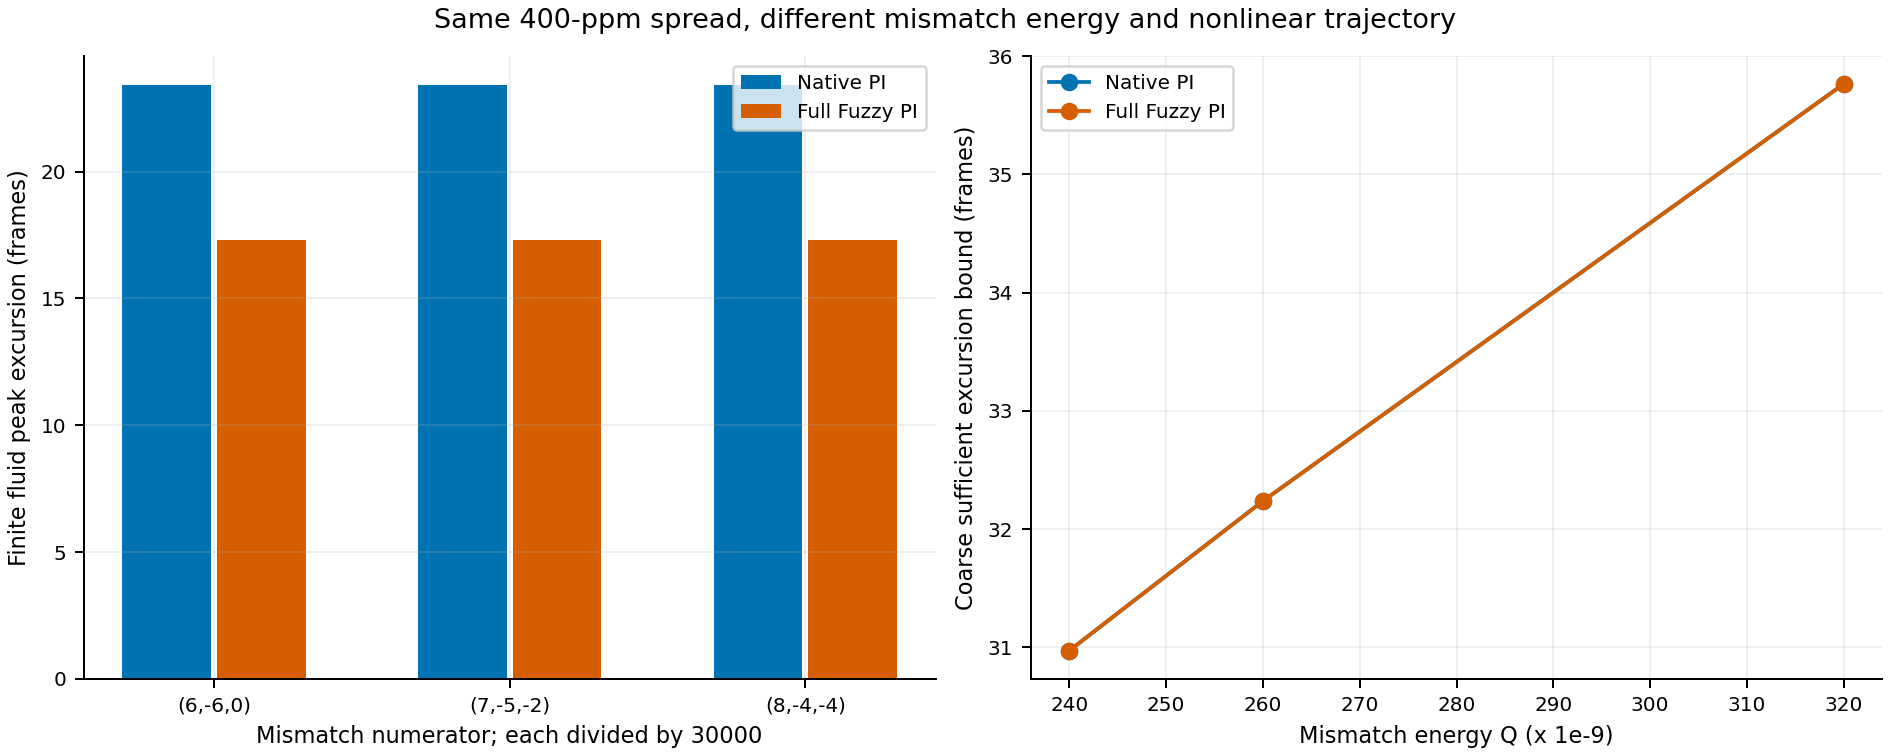
\includegraphics[width=0.94\textwidth]{images/safety_validation_20261105/direction_energy.png}
 \caption{Three equal-spread initializations with different mismatch
 energy. The energy identity is exact; a larger certificate radius
 does not imply a larger exact trajectory peak.}
 \Description{Mismatch energies and controller excursions for three 400-ppm directions.}
 \label{fig:safety_direction_energy}
\end{figure*}

The separately frozen annex adds four runs at $s=0.999,1.001$,
$z=20$. It independently recomputes every outward-arithmetic
cell of the uniform proof. Fuzzy's endpoint minima are approximately
2.703366 and 2.668520; PI's are $-3.380298$ and $-3.427105$.
The endpoint runs check implementation consistency. The 20-cell
coverage and infinite-tail argument, not endpoint interpolation,
establish the all-time statement over the entire interval.

\begin{figure*}[t]
 \centering
 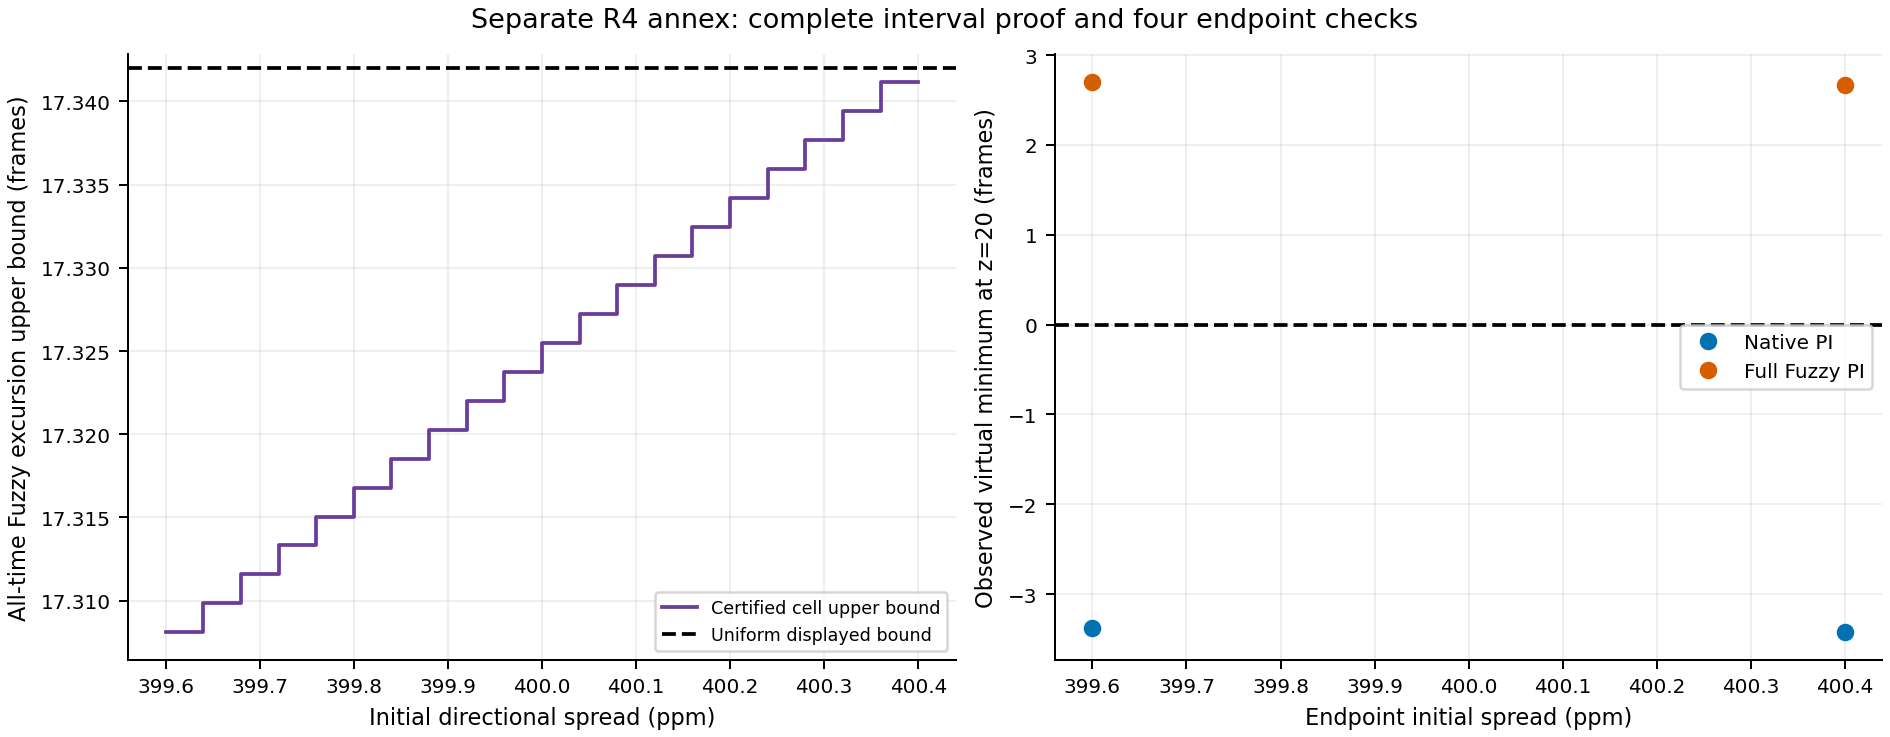
\includegraphics[width=0.94\textwidth]{images/safety_validation_20261105/uniform_annex_R4.png}
 \caption{Complete parameter-cell proof and direct endpoint checks.
 All 20 cells cover 399.6--400.4 ppm at the fixed mismatch direction.
 The maximum Fuzzy all-time bound is below 17.342; PI's minimum
 attained peak exceeds 23.3802976 throughout the interval.}
 \Description{Uniform interval bounds and four reference endpoint validations.}
 \label{fig:safety_uniform_interval}
\end{figure*}

All reference runs use bootstrap plus 2000 subsequent intervals.
Maximum translation residual is $6.83\times10^{-13}$ frame and
maximum phase residual $2.78\times10^{-12}$. The original comparison
tolerances are unchanged. Interpolation and rule replay are checked
separately from the exact proof certificate. The record contains
34 new reference trajectories, six cached sources and separate
proof/postprocessing evidence.

\subsection{All delayed Callisto cases}
The actual runs restore physical link latency 20, local polling
1000, execution delay 10 and integer events over $T=2001H$.
They fix $s=4$, initial phase 0.1, all capacities and gains above,
and use the original negative-time source history. For each $z$,
PI's target is $z$, Fuzzy's percentage setpoint is $100z/2048$,
and the marking is initial occupancy plus initial in-flight frames.
Each paired history and marking is identical. Guards are enabled
with reserve zero; observer, supervisory switching and anti-windup
are disabled. Requested/resolved settings are checked before
results are used.

\begin{table*}[t]
 \caption{All actual qualitative validation cases. Occupancy extrema
 include every integer event. Blocked time sums disabled-data-phase
 duration across nodes, rather than measuring elapsed network downtime.}
 \label{tab:safety_actual_all}
 \centering
 \begin{tabular}{@{}rllrrl@{}}\toprule
 $z$ & Controller & Buffer range / frames & Off episodes & Blocked node-ticks & First guard cause\\\midrule
 104 & PI & 10--198 & 0 & 0 & none\\
 104 & Fuzzy & 32--176 & 0 & 0 & none\\
 83 & PI & 0--166 & 5 & 61.0114 & empty input\\
 83 & Fuzzy & 11--155 & 0 & 0 & none\\
 64 & PI & 0--128 & 26 & 131.0456 & empty input\\
 64 & Fuzzy & 0--128 & 6 & 47.0093 & empty input\\
 1944 & PI & 1880--2008 & 26 & 131.0456 & delayed outgoing credit\\
 1944 & Fuzzy & 1880--2008 & 6 & 47.0093 & delayed outgoing credit\\
 1965 & PI & 1922--2008 & 51 & 222.1022 & delayed outgoing credit\\
 1965 & Fuzzy & 1922--2008 & 3 & 84.0205 & delayed outgoing credit\\
 1984 & PI & 1960--2008 & 5837 & 587.8914 & delayed outgoing credit\\
 1984 & Fuzzy & 1960--2008 & 1198 & 188.3495 & delayed outgoing credit\\\bottomrule
 \end{tabular}
\end{table*}

At $z=83$ PI's first input-empty guard occurs at
$t\simeq71844.671848$ ticks; five episodes sum to about 61.0114
blocked node-ticks. Fuzzy remains unstalled. The physical clock
continues to advance when data phase pauses, so physical-phase and
data-phase progress must be recorded separately.

\begin{figure*}[t]
 \centering
 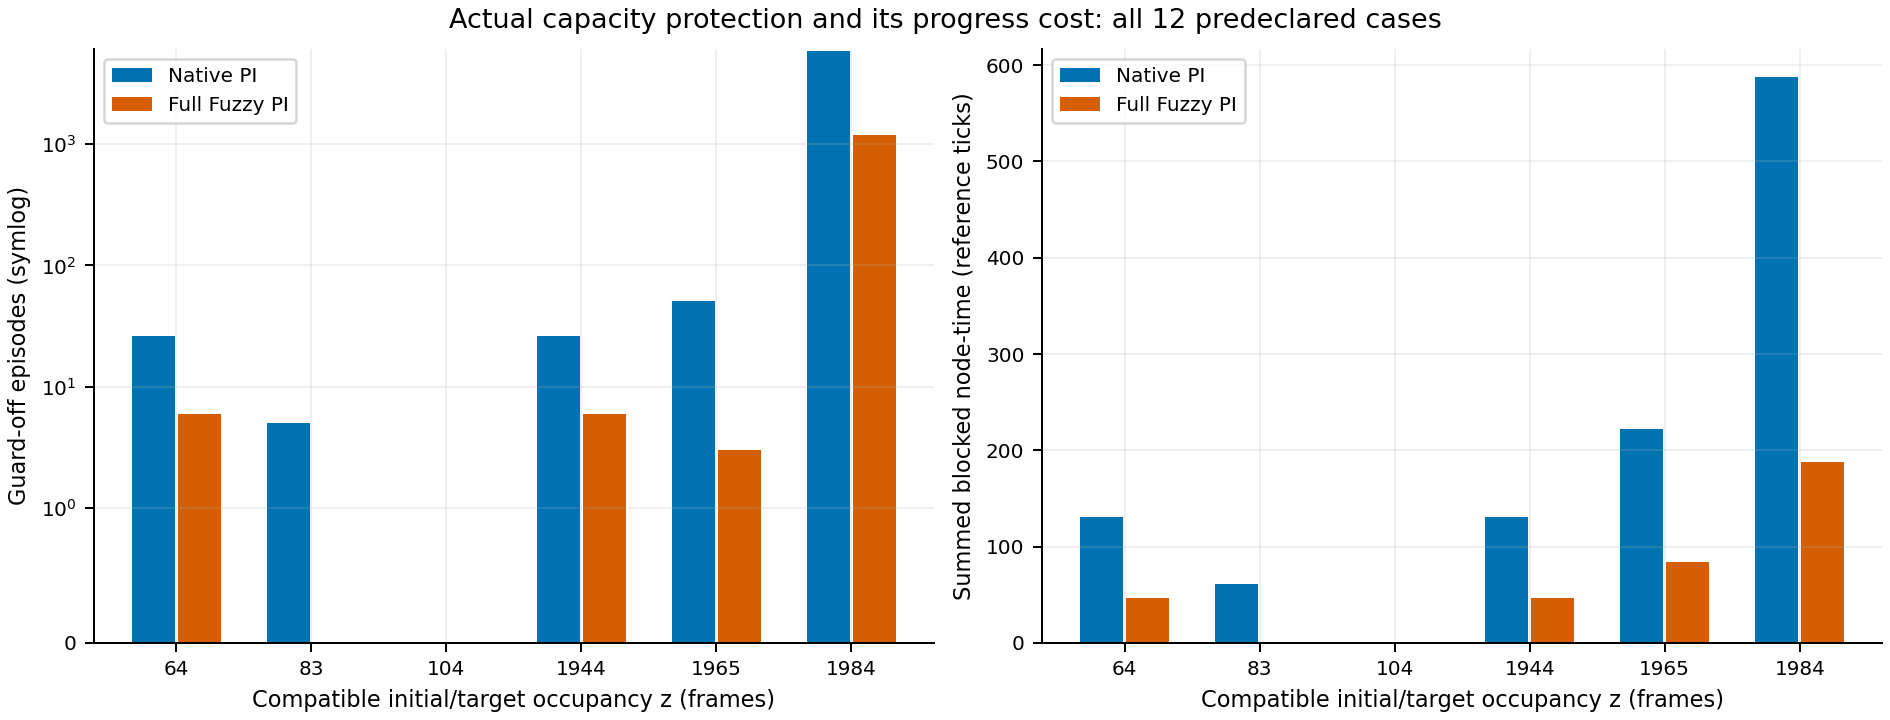
\includegraphics[width=0.94\textwidth]{images/safety_validation_20261105/actual_guard_comparison.png}
 \caption{Guard-off episodes and summed blocked node-time for every
 predeclared actual case. Three cases remain unstalled. Nine retain
 capacity with guard intervention; counts alone are not throughput.}
 \Description{Both normal and guarded outcomes, without omitting high-target cases.}
 \label{fig:safety_guard_comparison}
\end{figure*}

Upper-target cases do not reproduce the receiving-buffer mirror
of the zero-delay reference. In this runtime, used outgoing credit
is the UGN offset plus source sends minus causally delayed reverse
pops. Its initial value is $z+40$ although initial receiving occupancy
is $z$: the accounting includes forward in-flight data and delayed
reverse consumption knowledge. Full credit replay verifies its
capacity constraint. All upper-target cases guard while the maximum
physical receiving occupancy remains 2008. The first credit guards
at $z=1944$ occur at approximately 47886.861480 ticks (PI) and
57745.333282 ticks (Fuzzy), matching the corresponding $z=64$
lower-target cases. This explains the discrepancy without changing
gains. The observed 40-frame difference is specific to the declared
constant latency, history and protocol; it is not a general delay
margin or an all-time theorem for Callisto.

\begin{figure*}[t]
 \centering
 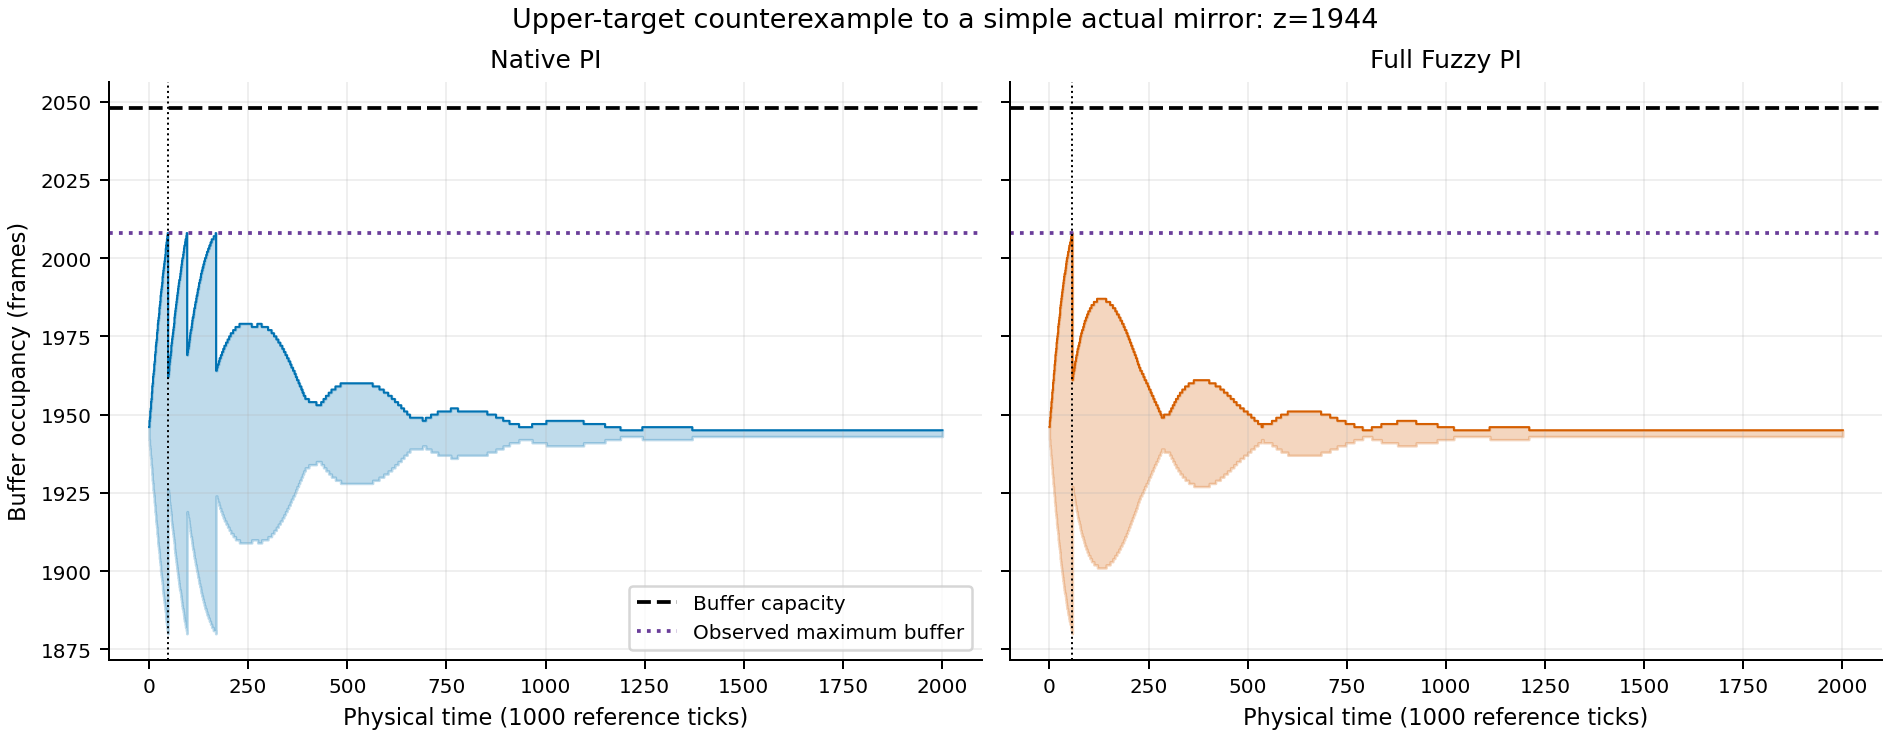
\includegraphics[width=0.94\textwidth]{images/safety_validation_20261105/actual_upper_credit.png}
 \caption{Actual upper-target credit constraint at $z=1944$.
 Credit readiness can stop sending before receiving occupancy reaches
 capacity. Forward in-flight frames and delayed reverse-pop knowledge
 prevent an occupancy-only upper/lower mirror argument.}
 \Description{Receiving buffers and delayed outgoing-credit guards in the upper-target case.}
 \label{fig:safety_upper_credit}
\end{figure*}

Every actual run has positive physical frequency (minimum 0.9993)
and no saturated correction. Complete integer arrival/pop replay
has zero occupancy mismatches; independent PI/25-rule command
reconstruction has maximum residual $1.09\times10^{-19}$.
Pre-first-guard measurements, command times and corrections agree
with the high-reserve source trajectory. Subsequent evolution is
from independent actual runs, not shifted old curves. All 12 runs
remain within inclusive physical capacity; the nine guarded cases
do not establish controller-only strict interior safety. At $z=1965$,
Fuzzy has fewer guard episodes but lower final data progress than
PI, so neither episode count nor blocked duration alone demonstrates
a throughput improvement.

\subsection{Claim--evidence separation}
Exact matrix/interval calculations certify the reference inner
domain, strict target-interval benefit and uniform narrow directional
interval. Reference simulation checks the original rules and model
identities. Delayed actual runs check whether the margin mechanism
persists, and expose an additional credit condition. They do not
certify arbitrary topology, delay, initial error at a fixed target,
globally optimal PI comparison, or application-payload logical
synchrony. Earlier random, burst and independently tuned comparisons
remain separate supplementary evidence in Appendix~\ref{app:evaluation}.

% Updated from completed, frozen experiments on 2026-11-03.
% Historical evaluation text is preserved as comments below the active section.
\section{Experimental Protocol and Supplementary Evidence}
\label{app:evaluation}
\noindent\textbf{Correspondence: Section~\ref{sec:evaluation}.} This appendix preserves the extended model, intermediate steps and supporting interpretation behind the corresponding main-text section.


\label{detail:sec:evaluation}

The evaluation connects the controller analysis to three distinct questions:
whether the continuous-clock implementation respects the PI calibration;
whether the nonlinear reference trajectories agree with the mathematical
analysis; and whether the proposed controller offers a measurable benefit
against independently tuned PI under shared delivery disturbances. We
separate matched-gain mechanism checks from equal-budget controller
selection, and reference-model certificates from Callisto simulation measurements.

\subsection{Experimental design and continuous-clock execution}
\label{detail:subsec:eval_design}

All Callisto simulations use the continuous-phase Callisto realization of
Section~\ref{detail:sec:fpi_controller}. Clock phases evolve continuously,
integer frame crossings determine buffer events, and measurements and
correction applications are scheduled by each node's local phase. There
is no common physical polling grid. Table~\ref{detail:tab:eval_setup} gives the
nominal plant; the startup stress study changes the uncontrolled frequencies
and reconstructs the associated negative-time histories explicitly.

\begin{table*}[t]
\caption{Nominal Callisto simulation configuration. Time is in physical reference
ticks except where local ticks are explicitly stated. Controller parameters
selected for independent tests are listed separately in
Table~\ref{detail:tab:eval_selected_gains}.}
\label{detail:tab:eval_setup}
\centering
\begin{tabular}{@{}ll@{}}\toprule
Parameter & Value\\\midrule
Topology & Three-node bidirectional triangle; six receiving buffers\\
Uncontrolled frequencies $\omega^u$ & $(1.0002,0.9998,0.9999)^\top$; initial spread 400 ppm\\
Initial phase; base frequency & $0.1$ at every node; $\omega_{\rm base}=29999/30000$\\
Capacity; initial occupancy; target & $C=2048$; $\beta_e(0)=\beta_e^*=1024$ frames\\
Initial in-flight frames; marking & 20 per channel; 1044 in the recorded convention\\
Nominal link latency & 20\\
Polling; control-execution delay & $p=1000$; $d_{\rm ctrl}=10$ local ticks\\
Execution constraints & $|u_i|\le0.01$; guards enabled; reserve zero; no anti-windup\\
Control law & Implemented integrate-first PI baseline or the complete incremental 25-rule Fuzzy law\\
Other mechanisms & Observer and supervisory mode switching disabled\\
Disturbance onset & $t_{\rm on}=2\times10^6$\\\bottomrule
\end{tabular}
\end{table*}

\paragraph{Evidence groups and data separation.}
The implementation check, M0, contains six matched pairs, or 12 actual
runs. An earlier fixed-preset burst campaign, M2, supplies a separate
mechanism diagnostic. The earlier fixed-preset random campaign, M3, is
development evidence and supplies no seeds to the new independent tests.
Its fixed-preset comparison did not support lower Fuzzy RMS against
moderate PI; the new study asks the different question of independently
selected controllers under an equal evaluation budget.
The new training study charges 192 slots, including four verified cached
M2 evaluations and 188 new Callisto simulation runs. Selection is frozen before 186
new held-out runs. A separately registered slower-disturbance study adds
107 Callisto simulation runs, including its engineering pilots, and the startup
study adds six. Its 32 synchronous fluid-reference trajectories are
reference calculations, not additional Callisto simulation runs. Old data, infeasible
candidates and repair records are retained in the evidence archive.

\paragraph{Shared delivery inputs.}
All controllers receive identical externally generated desired-latency
profiles within each comparison, verified by content hashes. Delay is
20 before onset, including the negative-time prehistory. Ordered arrivals
use the causal running-maximum envelope of
Section~\ref{detail:sec:fpi_controller}; a delay decrease may release an ordered
batch. The model does not impose a finite serialization rate.
For bounded random latency, the desired delay is $20+z_m$, where
\begin{align}
 z_0&=5\varepsilon_0,\nonumber\\
 z_m&=r_z z_{m-1}+(1-r_z)5\varepsilon_m,
 \quad r_z=e^{-1},\quad\varepsilon_m\sim\mathcal U[-1,1].
 \label{detail:eq:eval_random_profile}
\end{align}
Thus desired delay remains in $[15,25]$. The index $m$ counts physical
profile updates on a grid of spacing $T_c$, independently of controller
polling. Here $T_c$ denotes a profile-update interval, not an exactly
measured correlation time. The original two regimes use $T_c=1000$
and $10000$; the later confirmation study uses $100000$.

\subsection{Metrics, admissibility and comparison windows}
\label{detail:subsec:eval_metrics}

For $n$ nodes, let $\bar\omega(t)=n^{-1}\sum_i\omega_i(t)$ and define
the instantaneous across-node root-mean-square (RMS) disagreement as
\begin{align}
 \sigma_\omega(t)&=\sqrt{n^{-1}\sum_i[\omega_i(t)-\bar\omega(t)]^2},\nonumber\\
 \sigma_{\rm ppm}(t)&=10^6\sigma_\omega(t)/\omega_{\rm unit},
 \qquad\omega_{\rm unit}=1.
 \label{detail:eq:eval_disagreement_amplitude}
\end{align}
Parts per million (ppm) use the fixed normalized frequency unit, not
$\omega_{\rm base}$. For a physical-time window $W=[a,b)$ of duration
$T_W=b-a$, report
\begin{align}
 R_W&=\sqrt{T_W^{-1}\int_W\sigma_{\rm ppm}(t)^2\,dt},\nonumber\\
 I_W&=\int_W\sigma_{\rm ppm}(t)\,dt,
 \qquad P_W=\sup_{t\in W}\sigma_{\rm ppm}(t).
 \label{detail:eq:eval_frequency_metrics}
\end{align}
The integral absolute error (IAE) $I_W$ integrates RMS amplitude, rather
than the mean absolute node deviation. Frequency moments use complete
held-frequency intervals weighted by their physical durations.
The actual pairwise spread $\Delta_\omega=\max_i\omega_i-\min_i\omega_i$
is recorded separately. Although
$\Delta_\omega\le\sqrt{2n}\,\sigma_\omega$ pointwise, window RMS alone
does not establish a maximum transient-spread bound.

Buffer excursion, minimum two-sided headroom and mean command total
variation (TV) are
\begin{align}
 B_W^{\rm obs}&=\max_e\sup_{t\in[a,b]}|\beta_e(t)-\beta_e^*|,\nonumber\\
 H_W^{\rm obs}&=\min_e\inf_{t\in[a,b]}
                         \min\{\beta_e(t),C-\beta_e(t)\},
 \label{detail:eq:eval_buffer_metrics}\\
 \mathrm{TV}_W&=n^{-1}\sum_i
       \sum_{k:\,a\le t^a_{i,k}\le b}|u_{i,k}-u_{i,k-1}|.
 \label{detail:eq:eval_tv}
\end{align}
Buffer statistics reconstruct all integer crossings and ordered arrivals,
grouping simultaneous events and including the endpoint state. Sparse
plot samples do not determine extrema. TV includes both endpoints under
the frozen convention, so adjacent-window activities cannot be added
without treating the shared endpoint. TV measures command activity,
not hardware energy. Requested and applied corrections, saturation,
gate events, positive frequency and data-phase progress are checked
separately.

Before each post-centering disturbance, three consecutive $10^5$-tick
windows ending at onset must satisfy disagreement RMS at most 2 ppm,
each buffer's absolute mean bias at most two frames and standard
deviation at most one frame, common-frequency temporal standard
deviation at most 1 ppm and three-window mean range at most 1 ppm,
with positive progress and no intervention. These are finite
engineering centering criteria, not exact equilibrium. A training
candidate failing the same criteria in any required case remains
infeasible and consumes its assigned budget.

The original-regime tests use $W=[2\times10^6,4\times10^6)$ and tail
$[3.6\times10^6,4\times10^6)$. Each controller's own clean trajectory
is its same-parameter, nominal-delay counterfactual over the same
physical times. Common-frequency shift is reported relative to this
counterfactual, separately from relative synchronization. Strict
recovery requires the centering criteria for three consecutive windows
and a window-mean common frequency within 2 ppm of own clean. A return
not observed by the specified endpoint is right-censored, not assigned
a recovery time of zero or interpreted as permanent nonrecovery.

\subsection{Implementation and nonlinear-reference validation}
\label{detail:subsec:eval_implementation_reference}

M0 checks Proposition~\ref{detail:prop:fpi_equivalence} by replacing the Fuzzy
surface with its calibrated linear counterpart $F_0$, without changing
the continuous plant. Six pairs cover polling periods 100 and 1000,
initial frequency spreads 35 and 400 ppm, and capacity/target settings
$(2048,1024)$, $(512,128)$ and $(512,384)$ over $2\times10^5$ ticks.
Across 19,800 paired updates, the maximum correction difference is
$5.29\times10^{-18}$; physical/data phases, measurement vectors and
saved buffer counts agree, without saturation or guard intervention.
This checks initialization, integration order and gain mapping. It does
not replace the complete nonlinear law in the performance experiments.

The original 25-rule law is also evaluated directly on the synchronous,
zero-latency reference of Section~\ref{detail:sec:btd_reference}, with 2000
post-bootstrap updates. At the prescribed moderate-gain initialization,
the fluid buffer peak is approximately 17.314056818 frames, maximum
$|X|+|Y|$ is 0.090130790, maximum absolute correction is
$3.21398377\times10^{-4}$, and no contraction-envelope violation is
observed. Physical frequencies stay in $[0.9998,1.0002]$ including
startup. These finite numerical checks agree with the analysis; the
all-time comparison, Fuzzy below 17.315 versus PI approximately
23.403701 frames, follows from the interval-prefix and contracting-tail
proof in Theorem~\ref{detail:thm:btd_headroom}.

\paragraph{Rule verification.}
We reconstruct requested corrections from the saved inputs in all 299
new validation, slow-delivery and Callisto startup records. The maximum
residual is approximately $5.42\times10^{-20}$. This uses the complete
rule map and stored accumulator, not a sector surrogate. The earlier
M2 diagnostic additionally stays within $\Omega_5$, with observed
$\max(|X|+|Y|)=2.001888$, supporting application of
Proposition~\ref{detail:prop:fpi_central} to those measured inputs. This
diagnostic is retained separately from the independently selected
controllers: Fuzzy$_B$ reaches approximately 39.159 in the large
held-out burst. The full 25-rule law remains defined there, whereas
the central-region identity and the $\Omega_1$ reference witness do
not cover that whole trace. Same-input memory accounting is an
algebraic diagnostic, not an additional closed-loop $F_0$ experiment.

\subsection{Reference safety strata and Callisto startup transients}
\label{detail:subsec:eval_safety}

To vary initial mismatch without changing occupancy normalization,
capacity and targets remain fixed while
\begin{equation}
 \omega^u(s)=\frac{29999}{30000}\mathbf1
                 +s\frac{(7,-5,-2)^\top}{30000},
 \quad s\in\{0.5,1,2,4,8,16,32,64\}.
 \label{detail:eq:eval_stress_direction}
\end{equation}
Here $s$ is an initial-mismatch scale, with uncontrolled spread $400s$ ppm.
The reference uses the matched moderate coordinates
$(k_p,k_i)=(2\times10^{-6},5\times10^{-11})$, synchronous zero-latency
fluid execution and $H=h=30000000/29999$. Its 32 trajectories comprise
two controllers, eight scales and both unprotected virtual and
$0.01$-clipped variants. Each includes the bootstrap and 2000 subsequent
zero-order-hold intervals. The initial certificate energy scales as
$V_1(s)=s^2V_1(1)$; input-domain, buffer, positive-frequency and correction
conditions are checked jointly.

The largest grid point satisfying the common sufficient conditions is
$s=2$. At $s=4$, both reference trajectories remain normal over the
record although the certificate no longer guarantees them. At $s=32$,
unprotected reference requests first require actuator clipping; at
$s=64$, both virtual reference buffer trajectories violate capacity.
Figure~\ref{detail:fig:eval_reference_grid} distinguishes measured virtual
peaks from sufficient bounds. Failure of a sufficient condition is
inconclusive, rather than a prediction of instability.

\begin{figure*}[t]
\centering
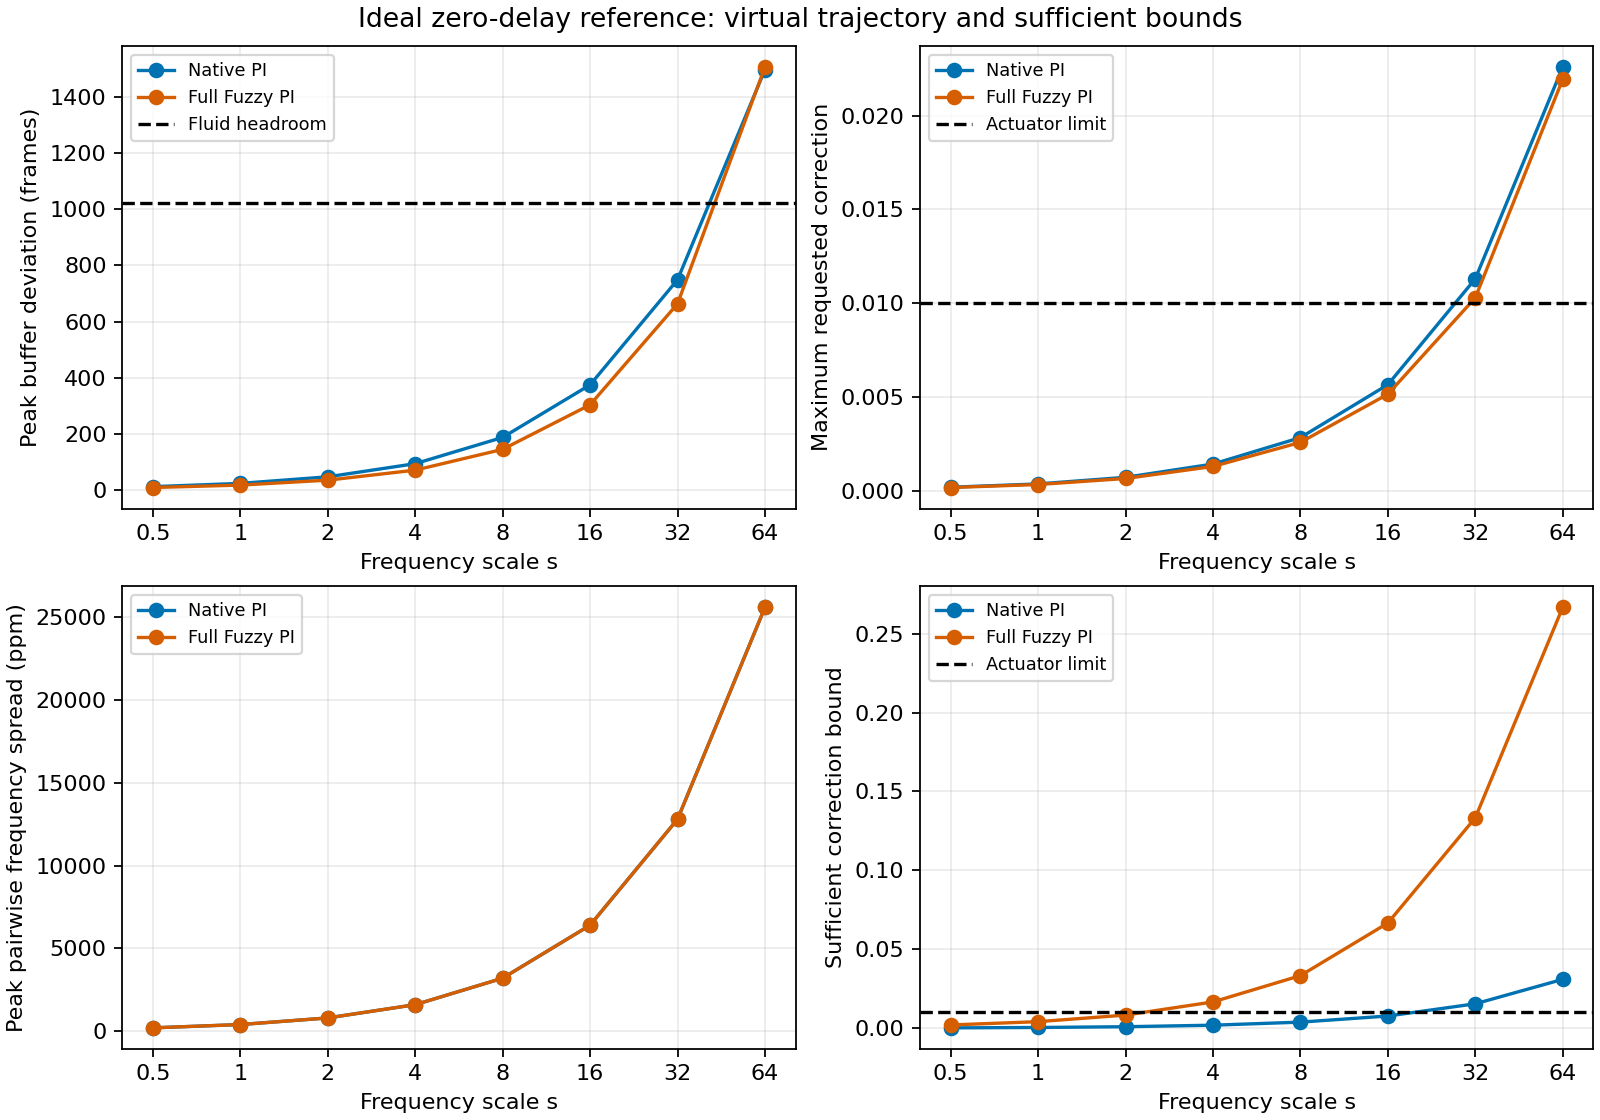
\includegraphics[width=0.97\textwidth]{images/evaluation_latest_20261103/reference_grid.png}
\caption{Synchronous zero-latency fluid-reference sweep at matched moderate
coordinates. Virtual trajectory peaks and analytical sufficient bounds
are distinct quantities. The dashed levels show fluid buffer headroom
and the correction limit; clipping and unprotected virtual trajectories
are archived separately. These are reference calculations, not actual
Callisto safety certificates.}
\Description{Four panels compare reference buffer peaks, requested corrections,
frequency spread and correction bounds over eight initial-mismatch scales.}
\label{detail:fig:eval_reference_grid}
\end{figure*}

Before running Callisto cases, the selection rule freezes three common
scales: 2, 4 and 32, representing certified, observed-safe uncertified,
and correction-constrained reference strata. Callisto restores
link latency 20 and local polling/control delay 1000/10. Its locked
startup horizon is $2001H\simeq2.001067\times10^6$ physical ticks,
rather than the $4\times10^6$ used for the disturbance tests. This
shorter horizon is an execution-plan deviation from the earlier
completion instruction and limits the empirical safety observation
accordingly. The six cases are startup stress tests, not
post-centering disturbance tests.

\begin{table}[t]
\caption{Callisto startup stress at matched moderate coordinates. Buffer
excursions include startup and all reconstructed events. Sat. counts
saturated control updates; every case has zero gate events and replay
mismatches.}
\label{detail:tab:eval_startup_safety}
\centering
\begin{tabular}{@{}rrrrr@{}}\toprule
 & & \multicolumn{2}{c}{Buffer excursion / frames} & Sat.\\
$s$ & Spread / ppm & PI & Fuzzy & PI / Fuzzy\\\midrule
2 & 800 & 47 & 37 & 0 / 0\\
4 & 1600 & 94 & 72 & 0 / 0\\
32 & 12800 & 750 & 664 & 176 / 85\\\bottomrule
\end{tabular}
\end{table}

Fuzzy has a smaller maximum actual buffer excursion at all three
selected scales (Table~\ref{detail:tab:eval_startup_safety}). At $s=4$, the
reduction is from 94 to 72 frames, approximately 23.4\%, with no
saturation or gate intervention. Figure~\ref{detail:fig:eval_startup_actual}
shows the associated frequency and occupancy transients. All six
records retain positive frequency, data progress and capacity
compliance. At $s=32$, Fuzzy also requests fewer saturated updates,
but 12800 ppm is a stress setting, not a typical hardware tolerance.
Its histories are initialized consistently: the faster source has
21 in-flight frames and marking 1045, whereas the other sources retain
20 and 1044. Both controllers receive identical histories at each scale.

\begin{figure*}[t]
\centering
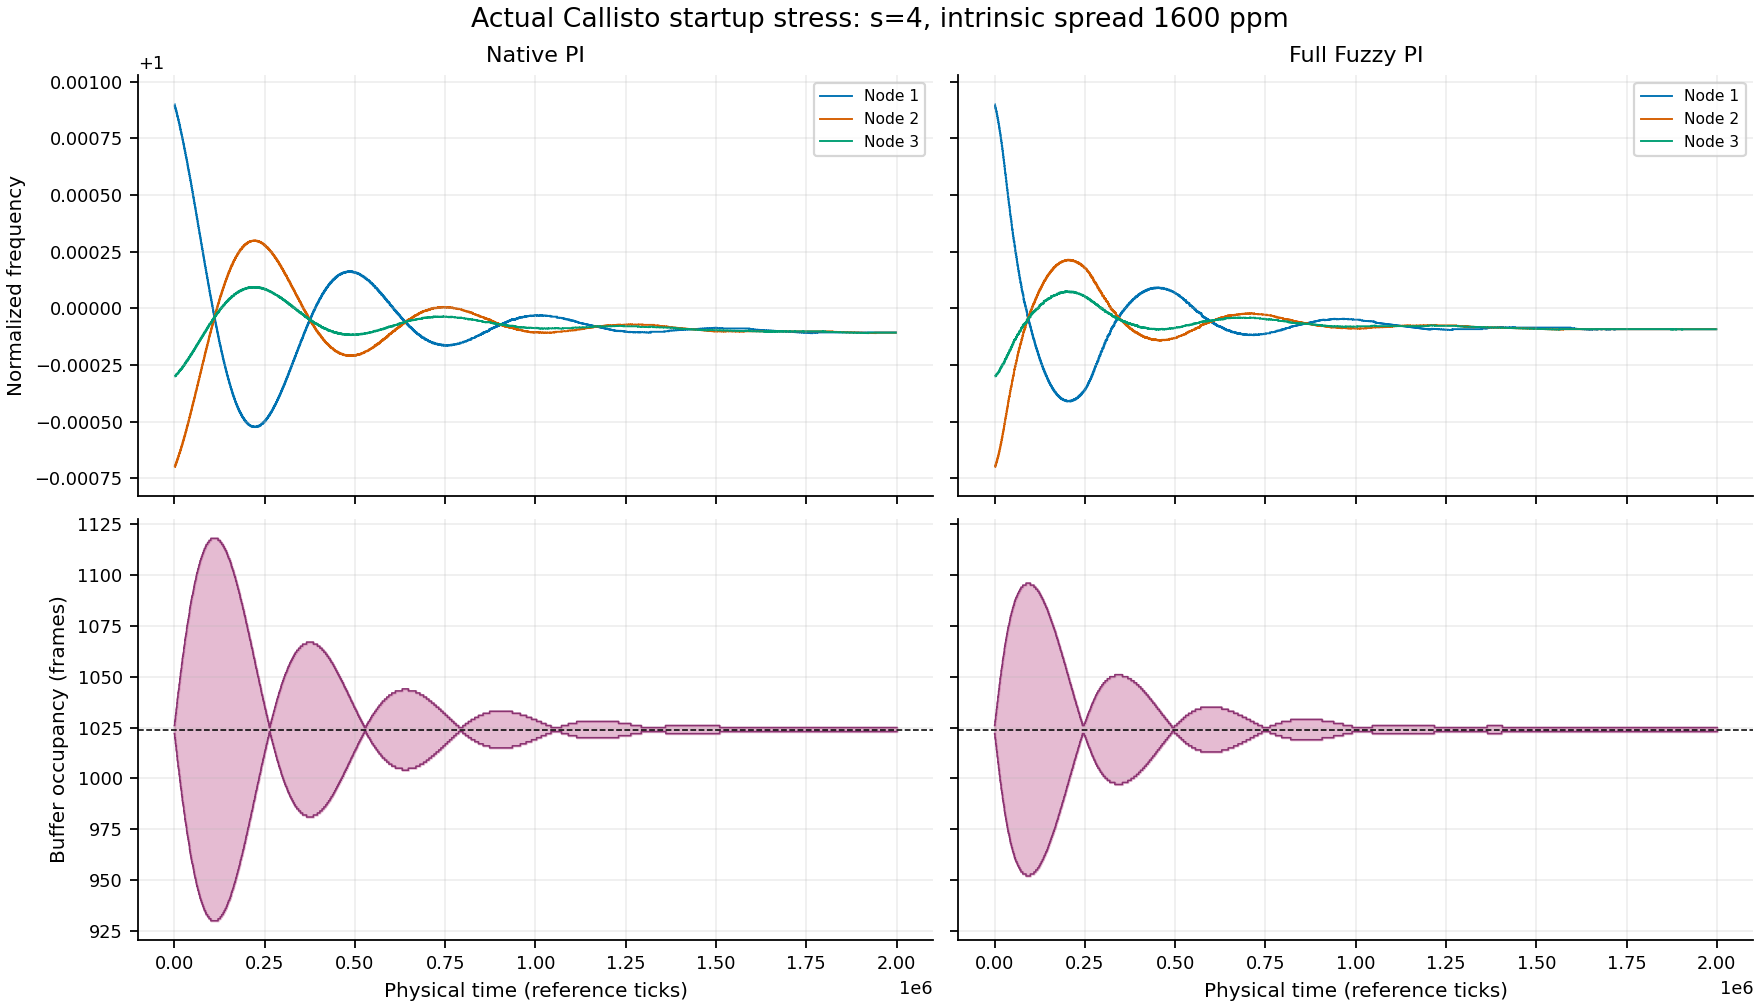
\includegraphics[width=0.97\textwidth]{images/evaluation_latest_20261103/actual_s4.png}
\caption{Continuous-phase Callisto startup at $s=4$ (1600 ppm),
with matched moderate coordinates. Upper panels show positive absolute
normalized frequencies using a $+1$ axis offset. Lower panels show the
minimum--maximum occupancy envelope across all receiving buffers, from
the complete crossing stream. Fuzzy reduces the maximum target
deviation from 94 to 72 frames over the stated startup horizon.}
\Description{PI and Fuzzy startup trajectories at the same frequency mismatch,
with absolute node frequencies and complete-event buffer-occupancy envelopes.}
\label{detail:fig:eval_startup_actual}
\end{figure*}

These observations show a smaller transient buffer demand at matched
gains, but do not transfer the reference theorem
to delayed, asynchronous, quantized execution. The recorded pairwise
spread remains a separate quantity. No hardware-based numerical
$\Delta_{\rm safe}$ is assumed; applying the reference spread corollary
would require an independently justified threshold exceeding $D(R)$.

\subsection{Equal-budget selection and independent random-latency tests}
\label{detail:subsec:eval_random}

\paragraph{Fixed search budget and selection.}
Each family uses the same 24-point grid,
\begin{align}
 k_p&\in\{1.5,2,2.5,3,4,6\}\times10^{-6},\nonumber\\
 k_i&\in\{1,2,5,10\}\times10^{-11}.
 \label{detail:eq:eval_gain_grid}
\end{align}
Fuzzy fixes $K_e=0.1$ and obtains $K_{\Delta e},K_u$ from the
calibration in Section~\ref{detail:sec:fpi_controller}; it receives no extra
shape-search dimension. Four training cases per candidate comprise
clean operation, a single-edge 20-tick delay increment lasting
$10^5$ ticks, and two random regimes using training seed 31001.
Both families therefore receive 96 evaluation slots. Four hash-verified
cached evaluations remain charged within the 192-slot total.
Nineteen PI and 22 Fuzzy candidates satisfy the same finite-run
admissibility requirements; all seven infeasible candidates are
retained without replacement.

Five training objectives are minimized separately: worst random-case
RMS, burst IAE, worst disturbance-window buffer excursion, peak absolute
common-frequency excursion from own clean, and worst mean command TV.
Each family's feasible Pareto set supplies a random-priority
representative, labeled $R$, and a burst-priority representative,
labeled $B$. The frozen lexicographic rule prioritizes random RMS for
$R$ and burst IAE for $B$, with the remaining objectives and candidate
identifier as declared tie breakers. One PI serves both priorities;
Fuzzy selects distinct representatives (Table~\ref{detail:tab:eval_selected_gains}).
Deduplication gives three candidates, without backfilling.

\begin{table*}[t]
\caption{Frozen representatives. The $k_p,k_i$ columns are PI baseline gains
for PI and calibrated PI coordinates for Fuzzy. $R$ and $B$ denote
random- and burst-priority selection; the candidates are not retuned on tests.}
\label{detail:tab:eval_selected_gains}
\centering
\begin{tabular}{@{}llrrrrr@{}}\toprule
Representative & Candidate & $k_p$ & $k_i$ & $K_e$ & $K_{\Delta e}$ & $K_u$\\\midrule
PI$_R$ = PI$_B$ & PI\_g05 & $2\times10^{-6}$ & $10^{-11}$ & --- & --- & ---\\
Fuzzy$_R$ & Fuzzy\_g02 & $1.5\times10^{-6}$ & $2\times10^{-11}$ & 0.1 & 7.499750 & $-1.638455\times10^{-5}$\\
Fuzzy$_B$ & Fuzzy\_g17 & $4\times10^{-6}$ & $10^{-11}$ & 0.1 & 39.998667 & $-8.192273\times10^{-6}$\\\bottomrule
\end{tabular}
\end{table*}

\paragraph{Held-out paired tests.}
Only after freezing selection are test profiles generated from seeds
41001--41030. All three candidates execute both original random
regimes and both held-out burst combinations, giving
$30\times2\times3+2\times3=186$ new Callisto simulation runs. All 186 complete
and satisfy the declared normal-admissibility checks, with no
engineering QA errors or complete-event replay mismatches. No seed
pair is excluded. Archived M3 seeds are not reused as held-out tests.

The primary random comparison is Fuzzy$_R$ versus PI$_R$. Let $\ell$
index independent seeds. Report the paired mean difference and mean
of per-seed ratios,
\begin{align}
 \widehat d&=\frac1{30}\sum_{\ell=1}^{30}
       (R_{W,\ell}^{\rm Fuzzy_R}-R_{W,\ell}^{\rm PI_R}),\nonumber\\
 \widehat r&=\frac1{30}\sum_{\ell=1}^{30}
       R_{W,\ell}^{\rm Fuzzy_R}/R_{W,\ell}^{\rm PI_R}.
 \label{detail:eq:eval_paired_ratio}
\end{align}
The ratio is not the ratio of group means. Confidence intervals (CIs)
use 20000 paired-seed percentile-bootstrap resamples, with fixed
resampling seeds 58001/58002. Pointwise 95\% intervals accompany
each endpoint; a joint statement about the two original regimes also
uses nominal Bonferroni-adjusted 97.5\% intervals per regime.
Time points, edges and bootstrap draws are not independent replications.

\begin{table*}[t]
\caption{Held-out original-regime tests: 30/30 admissible pairs per row.
Controller RMS entries are seed means in ppm. Difference is Fuzzy$_R$
minus PI$_R$; ratios are means of paired ratios. Brackets give pointwise
95\% paired bootstrap intervals.}
\label{detail:tab:eval_random}
\centering
\begin{tabular}{@{}lrrll@{}}\toprule
Profile grid & PI$_R$ RMS & Fuzzy$_R$ RMS & Difference / ppm [CI] & Paired ratio [CI]\\\midrule
$T_c=1000$ & 4.61355 & 3.83949 & $-0.77406$ [$-0.80767$,$-0.73992$] & 0.83217 [0.82484,0.83964]\\
$T_c=10000$ & 4.65204 & 4.28718 & $-0.36486$ [$-0.43523$,$-0.29464$] & 0.92150 [0.90630,0.93672]\\\bottomrule
\end{tabular}
\end{table*}

Table~\ref{detail:tab:eval_random} and Figure~\ref{detail:fig:eval_random_primary}
show reductions in disagreement RMS at both tested profile grids.
The mean paired relative improvements are 16.78\% and 7.85\%.
The nominal family-adjusted difference intervals are
$[-0.81274,-0.73483]$ and $[-0.44451,-0.28407]$ ppm, also below zero.
This supports an advantage of the selected Fuzzy scheme under the
declared finite-grid budget, plant and two input regimes. Because
the selected coordinates differ between families, it does not
isolate a same-gain inference-only effect or establish globally
optimal PI/Fuzzy performance.

\begin{figure*}[t]
\centering
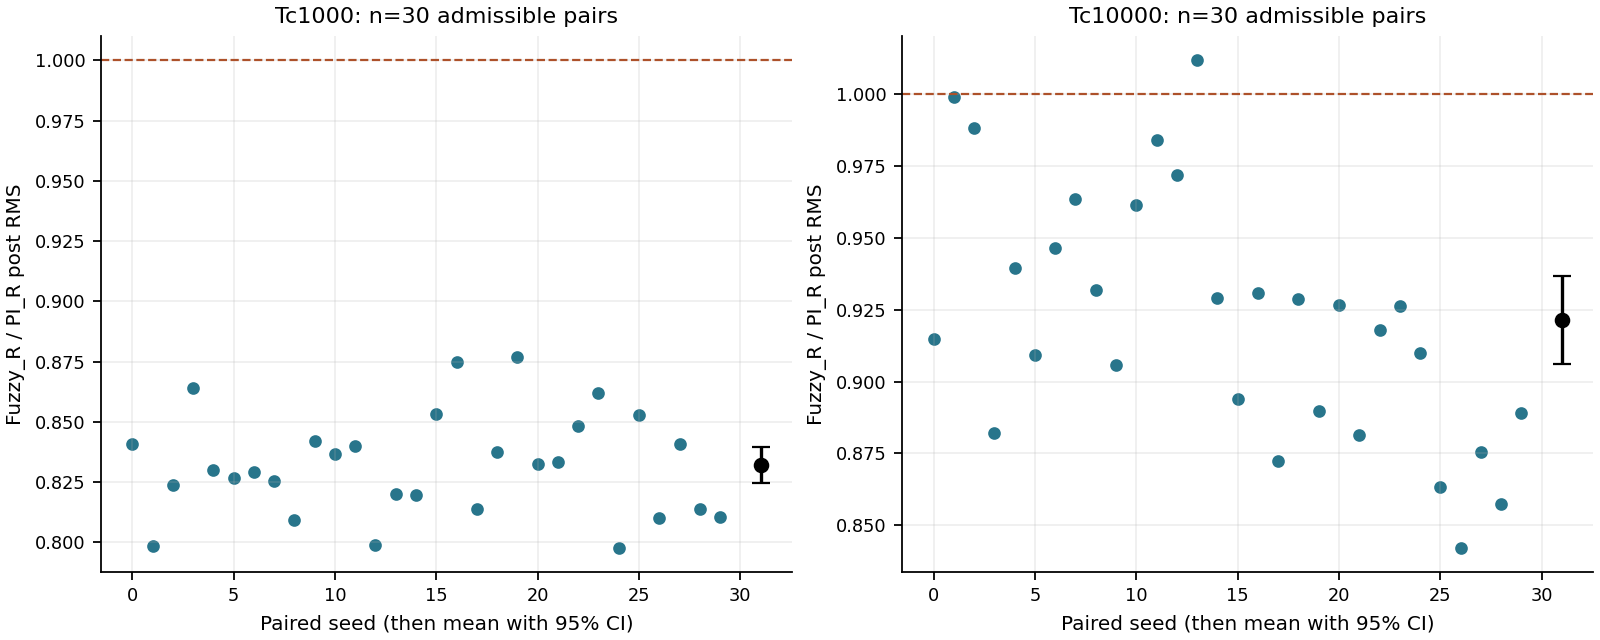
\includegraphics[width=0.97\textwidth]{images/evaluation_latest_20261103/paired_random_effects.png}
\caption{Independent paired Fuzzy$_R$/PI$_R$ RMS effects after equal-budget
selection. Each dot is one of 30 held-out seed pairs. The final black
marker is the mean paired ratio with a pointwise 95\% CI; the dashed
line denotes equal RMS. Individual seed outcomes and their aggregate
are both retained.}
\Description{Paired test-seed RMS ratios for profile intervals 1000 and
10000 ticks, with mean effects and bootstrap confidence intervals.}
\label{detail:fig:eval_random_primary}
\end{figure*}

\begin{figure*}[t]
\centering
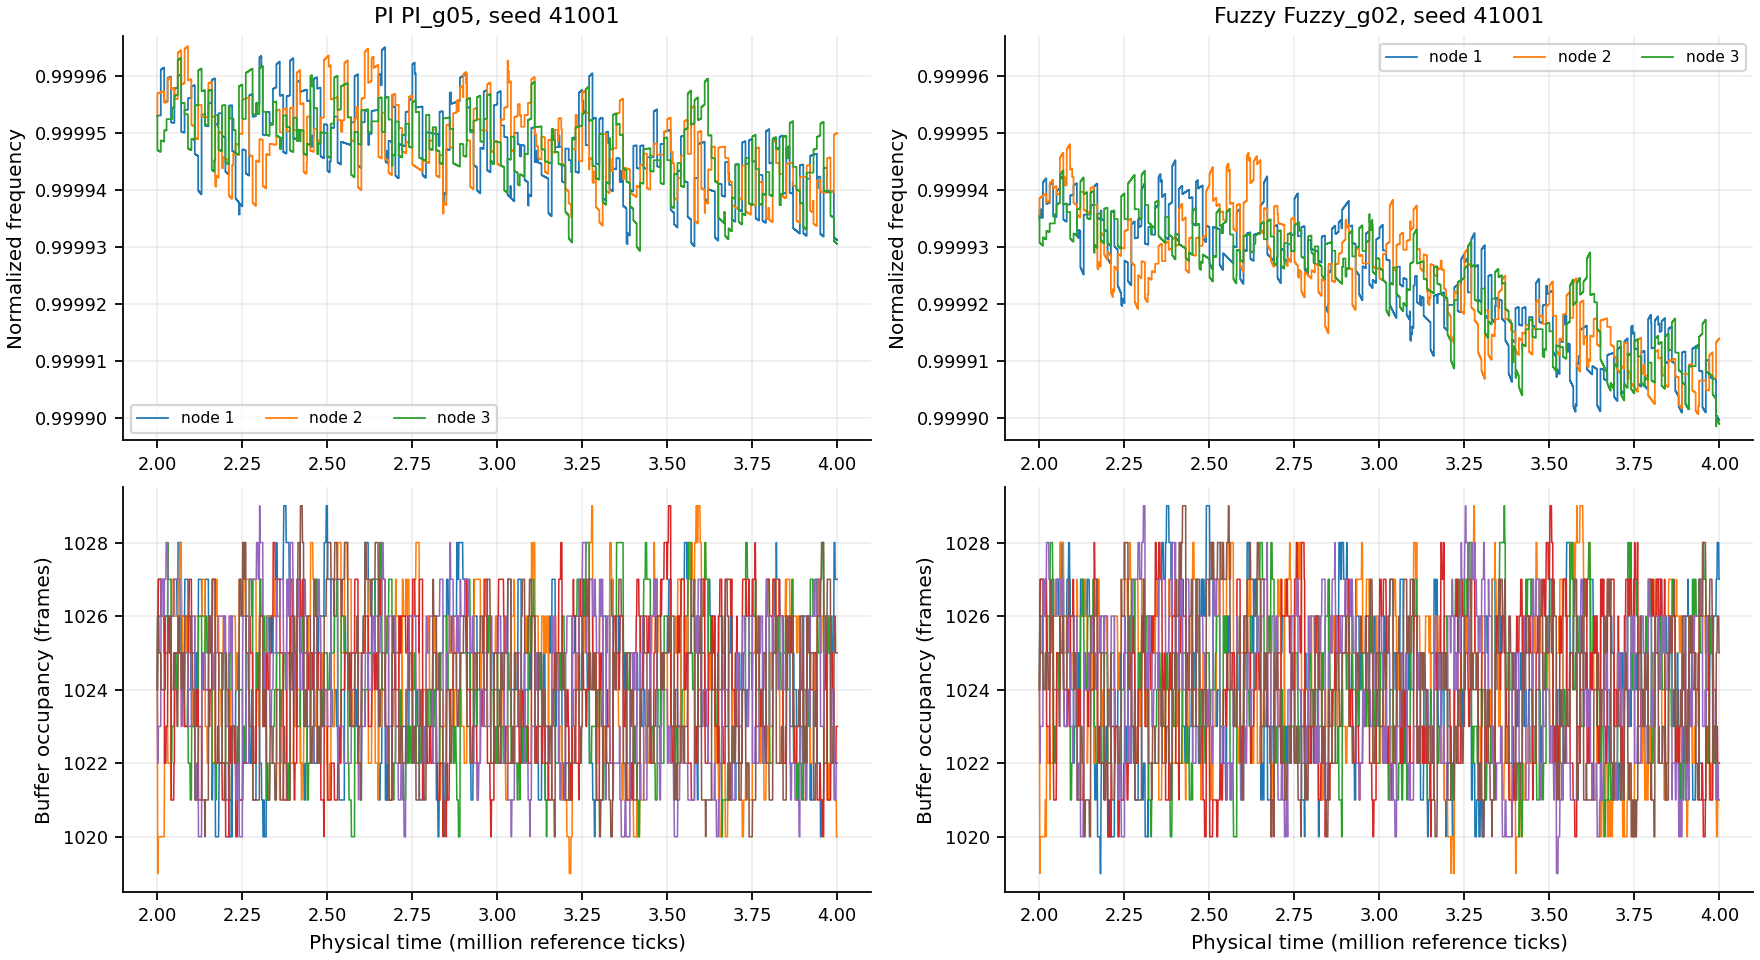
\includegraphics[width=0.97\textwidth]{images/evaluation_latest_20261103/raw_Tc10000.png}
\caption{Saved raw traces for the first held-out seed (41001) in the
$T_c=10000$ random experiment. Frequency uses held corrections and shared physical
time; buffer occupancy overview samples are for display. Reported
moments and buffer extrema instead use complete intervals and events.
The paired-seed statistics, rather than this one trace, support the
mean performance comparison.}
\Description{Shared-time node-frequency and buffer-occupancy
histories for the first held-out bounded-random delivery input.}
\label{detail:fig:eval_random_raw}
\end{figure*}

\paragraph{Activity and common-frequency cost.}
Mean per-node command TV decreases from 0.0102361 to 0.00782282 at
$T_c=1000$, and from 0.00112361 to 0.000906694 at $T_c=10000$
(PI$_R$ to Fuzzy$_R$). All selected candidates have at most six frames
of disturbance-window target deviation. However, Fuzzy$_R$ has larger
magnitude mean tail common-frequency shifts from own clean:
$-61.420$ versus $-15.692$ ppm, and $-31.933$ versus $-15.384$ ppm.
Thus reduced relative disagreement and command activity do not
imply improved absolute-frequency regulation. No absolute-frequency
reference loop is present.

\subsection{Held-out bursts and slower delivery changes}
\label{detail:subsec:eval_burst}

\paragraph{Burst-priority validation.}
The two predetermined held-out combinations are a 10-tick desired
delay increment lasting $10^4$ ticks on channel $2\to3$, and a
40-tick increment lasting $10^5$ ticks on $3\to1$, both beginning
at $2\times10^6$. They are distinct from the training combination.
For the larger burst, Fuzzy$_B$ lowers post-onset IAE from
$8.19241\times10^6$ to $3.62317\times10^6$ ppm$\cdot$ticks,
approximately 55.8\%, while matching the 40-frame buffer excursion.
Table~\ref{detail:tab:eval_heldout_bursts} retains both deterministic cases:
the improvement depends on the burst combination rather than holding
for every tested burst. These two cases do not supply seed-level CIs.

\begin{table}[t]
\caption{Both held-out burst-priority cases over
$[2\times10^6,4\times10^6)$. IAE is in $10^6$ ppm$\cdot$ticks;
buffer excursion is in frames. $A$ and $D$ denote desired delay
increment and its duration, respectively.}
\label{detail:tab:eval_heldout_bursts}
\centering
\begin{tabular}{@{}lrrrr@{}}\toprule
 & \multicolumn{2}{c}{IAE} & \multicolumn{2}{c}{Buffer excursion}\\
Case & PI$_B$ & Fuzzy$_B$ & PI$_B$ & Fuzzy$_B$\\\midrule
$A=10,D=10^4$ & 0.265814 & 0.352614 & 11 & 11\\
$A=40,D=10^5$ & 8.192410 & 3.623166 & 40 & 40\\\bottomrule
\end{tabular}
\end{table}

\paragraph{Ramp--hold--ramp inputs.}
A separate registered study freezes the selected gains and applies
a 20-tick delay increment on channel $1\to2$ using rise/fall times
$T_r\in\{10^4,10^5\}$ and hold times
$T_h\in\{10^5,10^6\}$. The four combinations all run to
$5.2\times10^6$ ticks. The end of the falling ramp is
$t_{\rm off}=2\times10^6+2T_r+T_h$; each case has its own
$[t_{\rm off},t_{\rm off}+2\times10^6)$ recovery window and
same-horizon clean counterfactual. A larger constant delay plateau
does not mean delivery stops throughout that plateau. The ramp
instead gives feedback time to act while the delivery imbalance forms.

For $T_r=10^5$, maximum buffer deviations are 19 frames for PI,
18 for Fuzzy$_R$ and 17 for Fuzzy$_B$. The slower formation of the
disturbance therefore provides another observed buffer-margin
benefit. Frequency RMS favors PI across the four ramp combinations,
and strict own-clean recovery is censored in all 12 ramp records.
Different disturbance durations are not pooled into a raw-IAE ranking;
these data support a resource/frequency tradeoff, not a faster-settling claim.

\paragraph{Separately registered slow-random confirmation.}
The slower grid $T_c=100000$ uses new seeds 51001--51030, unchanged
selected gains, the same bounded recursion, and
$W=[2\times10^6,5\times10^6)$ with tail
$[4.6\times10^6,5\times10^6)$. Each trace has 30 complete
profile blocks, which are not independent statistical replicates.
The study includes 105 matrix slots: three long-clean cases,
12 ramps and 90 random cases. Four matrix slots reuse qualified
pilot runs; 101 new main runs plus six pilots give 107 unique actual
runs. All matrix slots pass profile, nominal-prefix and event-replay
checks, with no excluded confirmation seed pairs.

This confirmation bounds the applicability of the original-regime
advantage: the mean paired Fuzzy$_R$/PI$_R$ RMS ratio is 1.33312
with pointwise 95\% CI [1.30337,1.36219], using 20000 paired
bootstrap resamples and fixed seed 59001. The mean paired difference
is $+1.53215$ ppm [1.39578,1.66175]. Slower variation alone therefore
does not extend the selected controller's RMS advantage. This confirmation
delimits the two original-regime benefits without changing their
registered primary endpoints or the frozen controller selection.

\subsection{Connection between analysis and measured benefits}
\label{detail:subsec:eval_support}

The evidence supports two benefits. First, nonlinear analysis at
matched gain coordinates proves a strict headroom improvement for the
prescribed fluid reference; Callisto startup tests at matched gains also show
smaller measured excursions at three fixed initial mismatches. Second,
equal-budget, independent selection yields lower disagreement RMS and
mean command activity in two held-out random regimes, while the
burst-priority representative reduces IAE in the larger held-out burst.
These are distinct statements with different gains, assumptions and
observation windows.

Their scope is explicit: common-frequency shift remains a cost, the
small burst and slower delivery tests delimit performance, and finite
Callisto records do not certify all-time safety or convergence. The
experiments do not establish a general safe-set inclusion, a globally
optimal comparator, payload-level functional logical synchrony, or
hardware energy savings. Positive phase progress and buffer compliance
show normal model execution; they are not a functional refinement proof.
Within these limits, the combined analysis and tests provide both a
mechanistic reason and independent empirical evidence for considering
the proposed Fuzzy PI law when transient buffer use and
disturbance-dependent synchronization performance matter.


% =====================================================================
% HISTORICAL EVALUATION BEFORE LATEST RESULTS -- ALL LINES COMMENTED
% Preserved for review; old fixed-preset tables/plots are not compiled.
% This archive does not replace the current confirmation-scope summary.
% =====================================================================
% % Evaluation assembled from completed evidence only, 2026-11-03.
% % No new Callisto runs, tuning/selection or PDF compilation is required.
% \section{Evaluation}
% \label{detail:sec:evaluation}
% 
% The evaluation addresses three questions. First, does the implementation
% respect the PI calibration and initialization derived in
% Section~\ref{detail:sec:fpi_controller}? Second, are the reference-model
% calculations consistent with the implemented nonlinear rule law? Third,
% how does the full Fuzzy controller compare with fixed PI baselines under
% post-centering delivery disturbances in continuous-phase Callisto?
% These questions require separate evidence: implementation equivalence,
% reference-model consistency, and finite-horizon performance do not
% establish the same claim.
% 
% \subsection{Evidence groups and comparison design}
% \label{detail:subsec:eval_design}
% 
% We use three completed actual-Callisto campaigns, denoted M0, M2 and M3,
% and separate fluid-reference calculations. M0 comprises six PI/linear-
% counterpart pairs, or 12 actual runs. M2 comprises four actual runs:
% PI and full Fuzzy, each with a clean trace and a single-edge latency
% burst. M3 comprises 180 actual validation runs: 30 independent paired
% seeds, two random-latency regimes and three fixed controllers. Six M3
% pilot runs are separate from the 180-run validation and are not treated
% as independent test replications. Reference calculations are not added
% to the actual-Callisto run count.
% 
% The primary performance comparison is moderate PI against the full
% Fuzzy law calibrated to its PI gain coordinates. M3 additionally includes
% a prespecified stronger PI candidate. All candidates are frozen within
% these campaigns. The linear surface $F_0$ is used only for the M0
% implementation check and explicitly labeled same-input diagnostics;
% M2 and M3 execute the full 25-rule nonlinear law. Axis matching controls
% scales and update conventions, but is not an assertion that either
% candidate is the best independently tuned controller.
% 
% \subsection{Continuous Callisto setup and delivery disturbances}
% 
% M2 and M3 use the continuous clock phases, local-clock scheduling
% and integer receiving-buffer counts described in
% Section~\ref{detail:sec:fpi_controller}. Table~\ref{detail:tab:eval_setup} gives their
% common configuration. Reported token counts represent counted frames
% in this model. There is no shared physical controller grid in
% these actual runs. The fixed native integration scale is
% $h=p/\omega_{\rm base}$, with the same convention in the calibrated
% Fuzzy controller. The initial intrinsic-frequency spread is 400 ppm of
% the normalized frequency unit.
% 
% \begin{table*}[t]
% \caption{Common configuration of the aligned burst and random-latency experiments.
% Time is measured in physical reference ticks unless specified as local ticks.}
% \label{detail:tab:eval_setup}
% \centering
% \begin{tabular}{@{}ll@{}}\toprule
% Parameter & Value\\\midrule
% Network & Three-node bidirectional triangle; six receiving buffers\\
% Intrinsic frequencies $\omega^u$ & $(1.0002,0.9998,0.9999)^\top$\\
% Initial phases; implementation base frequency & $0.1$ at every node; $\omega_{\rm base}=29999/30000$\\
% Capacity; initial occupancy; target & $C=2048$; $\beta_e(0)=\beta_e^*=1024$ frames\\
% Initial in-flight frames; delayed-run marking & 20 per channel; 1044 in the recorded convention\\
% Nominal physical path delay & 20\\
% Polling; control-execution delay & $p=1000$; $d_{\rm ctrl}=10$ local ticks\\
% Moderate PI $(k_p,k_i)$ & $(2\times10^{-6},5\times10^{-11})$\\
% Stronger fixed PI, M3 only & $(4\times10^{-6},5\times10^{-11})$\\
% Full Fuzzy $(K_e,K_{\Delta e},K_u)$ & $(0.1,3.9998666667,-4.0961365379\times10^{-5})$\\
% Execution policy & $u_{\max}=0.01$; shared guards enabled; reserve zero; no anti-windup\\
% Optional mechanisms & Observer and supervisory mode switching disabled\\
% Horizon; disturbance onset & $4\times10^6$; $t_{\rm on}=2\times10^6$\\\bottomrule
% \end{tabular}
% \end{table*}
% 
% \paragraph{Burst after nominal centering.}
% In M2, desired send-time latency on one directed channel, identified as
% $1\to2$ in the runtime configuration, changes from 20 to 40 during
% $[2\times10^6,2.1\times10^6)$ and returns to 20 afterwards. All other
% channels remain at 20. Each controller has its own clean counterfactual
% with latency 20 throughout. A controller's burst and clean histories
% match before onset, so their subsequent difference isolates the effect
% of the delivery disturbance for that controller. The nominal states
% of PI and Fuzzy are not required to be identical to each other.
% 
% \paragraph{Bounded random latency.}
% M3 uses fixed physical profile-update grids $T_c=1000$ and $10000$,
% independently of the unchanged controller polling period. For each
% generated link profile the bounded recursion is
% \begin{align}
%  z_0&=5\varepsilon_0,\nonumber\\
%  z_m&=r_z z_{m-1}+(1-r_z)5\varepsilon_m,
%  \qquad r_z=e^{-1},\quad\varepsilon_m\sim\mathcal U[-1,1],
%  \label{detail:eq:eval_random_profile}
% \end{align}
% with desired delay $20+z_m\in[15,25]$ after onset. Here $m$ indexes
% profile updates, not controller measurements. The designation $T_c$
% refers to the profile grid, not an exactly measured correlation time.
% Before onset, including negative-time prehistory, delay is 20. Seeds
% 20001--20030 are independent validation replications; pilot seed 1001
% is excluded. For each seed and regime, all three controllers receive
% identical externally generated profile content.
% 
% Both disturbance families use the declared causal running-maximum
% arrival envelope. Frame order is retained and a delay decrease can
% release an ordered batch. No finite serialization-rate model, frame
% dropout or application-payload experiment is included. These are
% specified transport stress models rather than claims about arbitrary
% network traffic.
% 
% \subsection{Metrics, windows and finite-run admissibility}
% \label{detail:subsec:eval_metrics}
% 
% \paragraph{Disagreement and absolute frequency.}
% For the instantaneous common frequency $\bar\omega(t)=n^{-1}\sum_i\omega_i(t)$,
% define
% \begin{align}
%  \sigma_\omega(t)&=\sqrt{\frac1n\sum_i[\omega_i(t)-\bar\omega(t)]^2},\nonumber\\
%  s(t)&=10^6\sigma_\omega(t)/\omega_{\rm unit},\qquad\omega_{\rm unit}=1.
%  \label{detail:eq:eval_disagreement_amplitude}
% \end{align}
% Thus $s$ is an instantaneous across-node root-mean-square (RMS)
% amplitude in parts per million (ppm). Its normalization is the fixed
% unit frequency, not $\omega_{\rm base}$ or the reference ramp frequency
% used in Section~\ref{detail:sec:btd_reference}. For $W=[t_s,t_e)$ with duration
% $T_W=t_e-t_s$, report
% \begin{align}
%  R_W&=\sqrt{T_W^{-1}\int_W s(t)^2\,dt},\nonumber\\
%  I_W&=\int_W s(t)\,dt,\qquad P_W=\sup_{t\in W}s(t).
%  \label{detail:eq:eval_frequency_metrics}
% \end{align}
% The recorded integral absolute error (IAE) is $I_W$, the integral of
% this nonnegative RMS amplitude. It is not the integral of the mean
% absolute node deviation. Moments are integrated over complete held-
% frequency intervals using physical-duration weights, not uniform
% averages of controller updates.
% 
% These quantities must also be distinguished from the pairwise spread
% $\Delta_\omega(t)=\max_i\omega_i(t)-\min_i\omega_i(t)$ of
% Section~\ref{detail:sec:btd_reference}. Cauchy--Schwarz gives
% $\Delta_\omega(t)\le\sqrt{2n}\,\sigma_\omega(t)$, but a window RMS
% does not bound a pointwise transient by itself. We retain positive-
% frequency checks and common-frequency diagnostics separately. For M2,
% a supplementary descriptive spread calculation uses the already saved
% shared-time frequency intervals; it is not a new simulation or a
% preregistered primary endpoint.
% 
% \paragraph{Buffer excursion and control activity.}
% Measured buffer excursion and remaining headroom are
% \begin{align}
%  B_W^{\rm obs}&=\max_e\sup_{t\in[t_s,t_e]}|\beta_e(t)-\beta_e^*|,\nonumber\\
%  H_W^{\rm obs}&=\min_e\inf_{t\in[t_s,t_e]}
%                      \min\{\beta_e(t),C-\beta_e(t)\}.
%  \label{detail:eq:eval_buffer_metrics}
% \end{align}
% Every integer phase crossing and ordered arrival is reconstructed.
% Simultaneous events are grouped under the frozen convention, and
% buffer extrema include the right-endpoint state. Display samples are
% not the source of peak or moment statistics. Conservative reference
% certificates are not substituted for measured extrema.
% Mean per-node command total variation (TV) is
% \begin{equation}
%  \mathrm{TV}_W=\frac1n\sum_i
%        \sum_{k:\,t_s\le t^a_{i,k}\le t_e}|u_{i,k}-u_{i,k-1}|.
%  \label{detail:eq:eval_tv}
% \end{equation}
% Activity uses inclusive endpoints in the frozen protocol; adjacent
% subwindow activities must not be added without handling their shared
% boundary. All evaluated M2/M3 runs have zero recorded saturation, so
% requested and applied command increments coincide. TV is a command-
% activity measure, not measured hardware energy or computational cost.
% 
% \paragraph{Windows and recovery.}
% The primary disturbance window is $[2\times10^6,4\times10^6)$.
% M2 additionally separates burst ON and post-OFF intervals at
% $t_{\rm off}=2.1\times10^6$. Before onset, both M2 controllers and all
% M3 cases pass three consecutive $10^5$-tick nominal windows: disagreement
% RMS at most 2 ppm, each buffer's absolute mean bias at most two frames
% and standard deviation at most one frame, common-frequency temporal
% standard deviation at most 1 ppm and three-window mean range at most
% 1 ppm, with positive frequencies/progress and no intervention. These
% are finite engineering centering criteria, not exact equilibrium.
% 
% M2 component recovery requires these criteria in three consecutive
% post-OFF windows. Strict recovery additionally requires the window-mean common
% frequency to return within 2 ppm of that controller's own clean
% trajectory over the same physical-time window. A missing qualifying return by
% $4\times10^6$ is right-censored; it is neither zero recovery time nor
% proof of permanent nonrecovery. M3 uses $[3.6\times10^6,4\times10^6)$
% for tail diagnostics. The separate M2 memory decomposition below uses
% $[3.7\times10^6,4\times10^6)$.
% 
% \subsection{Implementation equivalence and reference consistency}
% \label{detail:subsec:eval_implementation_reference}
% 
% M0 varies polling over 100 and 1000 local ticks, initial frequency
% spread over 35 and 400 ppm, and includes capacity/target settings
% $(2048,1024)$, $(512,128)$ and $(512,384)$ across its six matched pairs.
% All pairs use constant path delay 20, execution delay 10 and a
% $2\times10^5$-tick horizon. Target-centered percentages are used for
% non-midpoint targets. Across 19,800 paired updates, the maximum
% requested/applied correction difference is $5.29\times10^{-18}$.
% Physical and data phases coincide at all evaluated union knots, with
% identical measurement vectors and saved-time buffer counts. No guard
% intervention or saturation is recorded. This supports the implemented
% calibration, integration order and constructor treatment of
% Proposition~\ref{detail:prop:fpi_equivalence}; it is not a nonlinear-Fuzzy
% performance result or a general runtime-equivalence proof.
% 
% Separate previously completed reference calculations call the original
% 25-rule Fuzzy update directly, rather than advance the plant with a
% sector surrogate. Two trajectories use moderate and stronger gain
% coordinates, each with 2000 post-bootstrap updates. For the moderate
% configuration corresponding to Section~\ref{detail:sec:btd_reference}, the
% observed maximum fluid buffer deviation is approximately 17.314056818
% frames, maximum $|X|+|Y|$ is 0.090130790, and maximum absolute correction
% is $3.21398377\times10^{-4}$. There are no observed stepwise
% contraction-envelope violations; frequencies remain in
% $[0.9998,1.0002]$ including startup. These numerical checks are
% consistent with the reference certificate, but the all-time guarantee
% and strict PI comparison come from the interval-prefix and certified-
% tail argument of Theorem~\ref{detail:thm:btd_headroom}, not from a finite
% floating-point trajectory. The reference marking is 1024; the delayed
% actual runs' marking is 1044.
% 
% \subsection{Response to a post-centering latency burst}
% \label{detail:subsec:eval_burst}
% 
% Table~\ref{tab:eval_burst} reports the aligned moderate-gain comparison.
% Figure~\ref{fig:eval_burst_overview} shows the shared-time frequency,
% buffer and latency traces, including the clean counterfactuals.
% Fuzzy reduces RMS-amplitude IAE by 1.864\% and mean command TV by
% 15.938\%. Its disagreement RMS is 0.096\% higher, instantaneous RMS
% peak is 2.396\% higher, and target-referenced buffer excursion is one
% frame larger. These endpoints establish a tradeoff at this deterministic
% operating point, not a uniform disturbance-rejection advantage.
% 
% \begin{table*}[t]
% \caption{M2 metrics over $[2\times10^6,4\times10^6)$ unless stated otherwise.
% Lower is preferable except for buffer headroom. The spread row is a
% supplementary descriptive calculation; no engineering spread threshold
% was predeclared for these runs.}
% \label{tab:eval_burst}
% \centering
% \begin{tabular}{@{}lrr@{}}\toprule
% Metric & Moderate PI & Full Fuzzy\\\midrule
% Disagreement RMS $R_W$ / ppm & 9.67059 & 9.67988\\
% Instantaneous RMS peak $P_W$ / ppm & 32.59447 & 33.37534\\
% RMS-amplitude IAE $I_W/(10^6\ \mathrm{ppm\cdot ticks})$ & 9.94254 & 9.75722\\
% Supplementary peak pairwise spread / ppm & 69.14830 & 70.89161\\
% Buffer excursion $B_W^{\rm obs}$ / frames & 20 & 21\\
% Minimum lower / upper buffer headroom / frames & 1004 / 1017 & 1003 / 1017\\
% Mean command TV / $10^{-4}$ & 2.62204 & 2.20415\\
% Largest command increment / $10^{-5}$ & 4.10000 & 4.21763\\
% Peak common-frequency difference from own clean / ppm & 60.61864 & 61.26423\\
% Component entry / confirmation after OFF / $10^6$ ticks & 0.8 / 1.1 & 0.8 / 1.1\\
% Strict own-clean recovery by the horizon & Censored & Censored\\
% Full-run buffer excursion, including startup / frames & 24 & 21\\\bottomrule
% \end{tabular}
% \end{table*}
% 
% \begin{figure*}[t]
% \centering
% 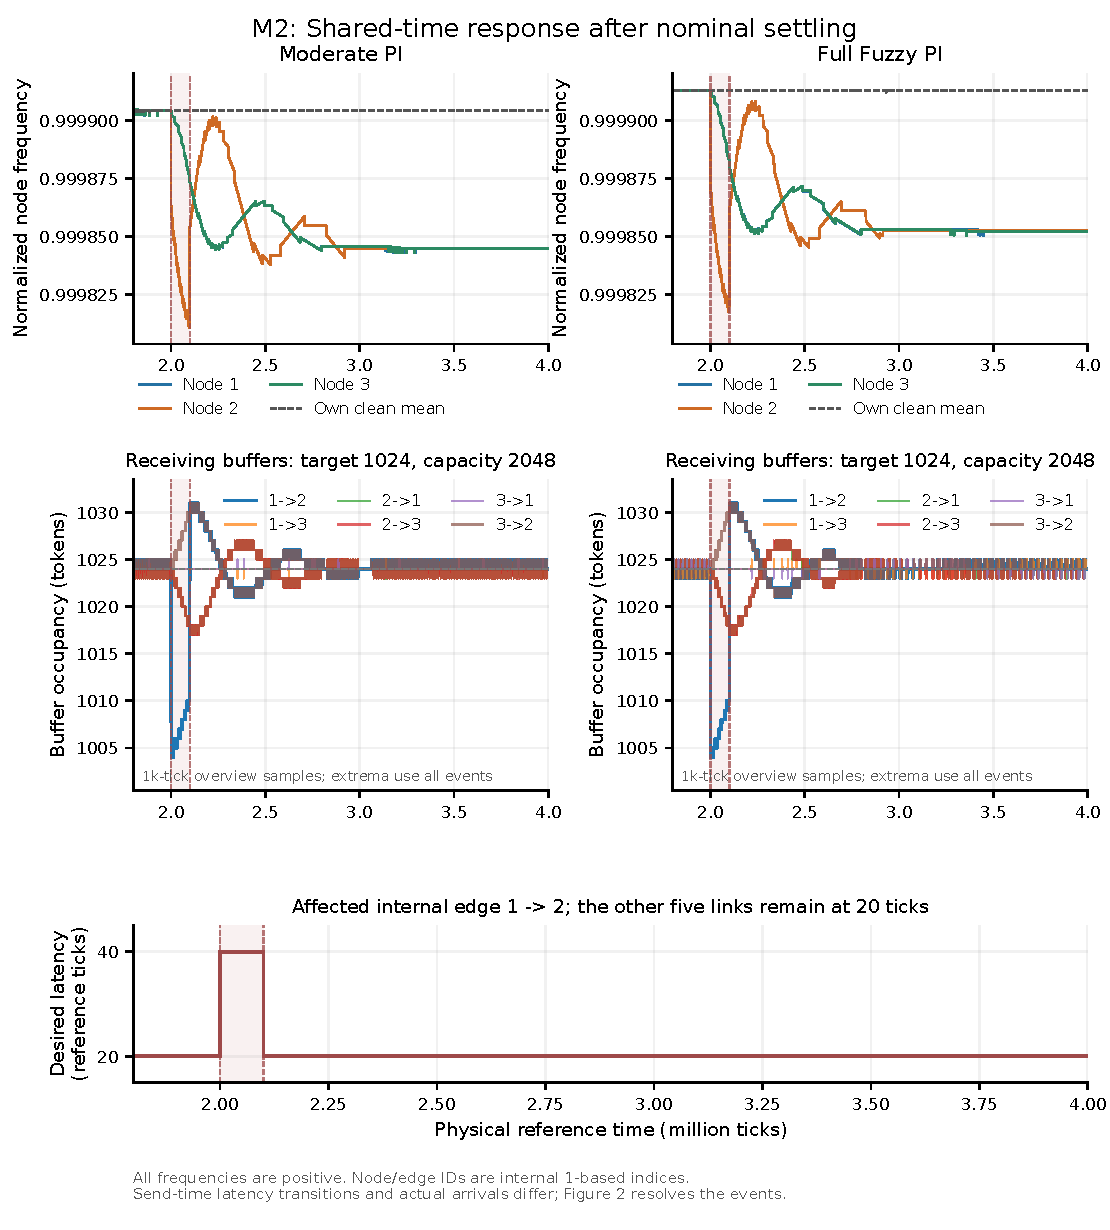
\includegraphics[width=0.97\textwidth]{images/evaluation_20261103/m2_shared_time_response.pdf}
% \caption{Aligned post-centering burst experiment. Continuous-phase Callisto
% uses the fixed moderate PI coordinates and their full-Fuzzy calibration.
% Both controllers have their own clean counterfactual. Desired latency on
% one directed channel changes from 20 to 40 during
% $[2\times10^6,2.1\times10^6)$. Frequency histories use held corrections;
% buffer overview samples are for display, while reported buffer statistics
% come from the complete reconstructed event stream.}
% \Description{Shared-time overview of node frequencies, six receiving-buffer
% occupancies, and the imposed path-latency burst for PI and Fuzzy PI.}
% \label{fig:eval_burst_overview}
% \end{figure*}
% 
% Both controllers remain within capacity with positive frequency and
% continuing logical phase progress, without recorded guard or saturation
% intervention. Including startup, the full-run maximum deviation is
% 24 frames for PI and 21 for Fuzzy. This is a favorable Fuzzy endpoint
% for that full window, whereas the post-onset peaks are 20 and 21.
% Changing the window changes the ranking, so neither figure is used as
% a replacement for the other. Capacities are far from exhaustion.
% 
% Both first enter the window-qualified component recovery band at
% $2.9\times10^6$ and confirm it at $3.2\times10^6$. Thus the experiment
% does not show faster Fuzzy settling under this criterion. Strict
% own-clean recovery is censored for both. In the memory-diagnostic
% tail, the common-frequency changes relative to own clean are
% $-59.40198$ ppm for PI and $-60.51069$ ppm for Fuzzy. A stationary
% common frequency, frequency agreement between nodes, return to own
% clean, and return to frequency one are different properties.
% 
% \subsection{Observed nonlinear mechanism and the first buffer peak}
% \label{subsec:eval_mechanism}
% 
% The M2 rule replay agrees with the full nonlinear implementation.
% All sampled Fuzzy input pairs remain in $\Omega_5$, with disturbance-window
% maximum $|X|+|Y|=2.001888$. The central identity of
% Proposition~\ref{detail:prop:fpi_central} therefore applies to those observed
% updates. However, this trajectory does not stay in the smaller
% $\Omega_1$ input diamond used by the reference example. This is not
% evidence of a sector violation or instability; it is another reason,
% besides asynchrony, delay and quantization, that the example's
% invariant-region certificate is not a certificate for this actual burst.
% 
% The Section~\ref{detail:sec:fpi_controller} decomposition into proportional,
% integral-like and accumulated nonlinear-residual terms reproduces the
% requested correction with maximum residual is approximately
% $6.46\times10^{-18}$. In the diagnostic tail, the Fuzzy own-clean
% common-frequency shift decomposes into
% \begin{equation}
%  -60.51069=-57.61859-2.89210\quad\mathrm{ppm},
%  \label{eq:eval_memory_accounting}
% \end{equation}
% where the two terms are the linear integral-like contribution and
% nonlinear memory; the proportional contribution is zero. PI's
% $-59.40198$ ppm shift is its integral contribution. This is exact
% same-trajectory accounting up to numerical arithmetic, not an
% independently evolving $F_0$ closed-loop ablation or a unique causal
% explanation of the physical common frequency.
% 
% Figure~\ref{fig:eval_mechanism} also resolves the first buffer peak.
% PI and Fuzzy first attain their disturbance-window maximum target deficits at
% ON$+39.105$ and ON$+40.731$ ticks, whereas their first changed commands
% relative to own clean occur at ON$+155.216$ and ON$+155.841$.
% At the respective first extrema, clean/burst occupancies are
% 1024/1004 for PI and 1023/1003 for Fuzzy. Both same-time
% clean-minus-burst deficits are therefore 20 frames: target deficits of
% 20 and 21 combine that delivery deficit with clean-state offsets of
% zero and one. Consequently the first attainment is not a measurement
% of post-burst feedback effectiveness. The minimum is revisited later;
% we do not claim that every peak instance precedes feedback.
% 
% \begin{figure*}[t]
% \centering
% 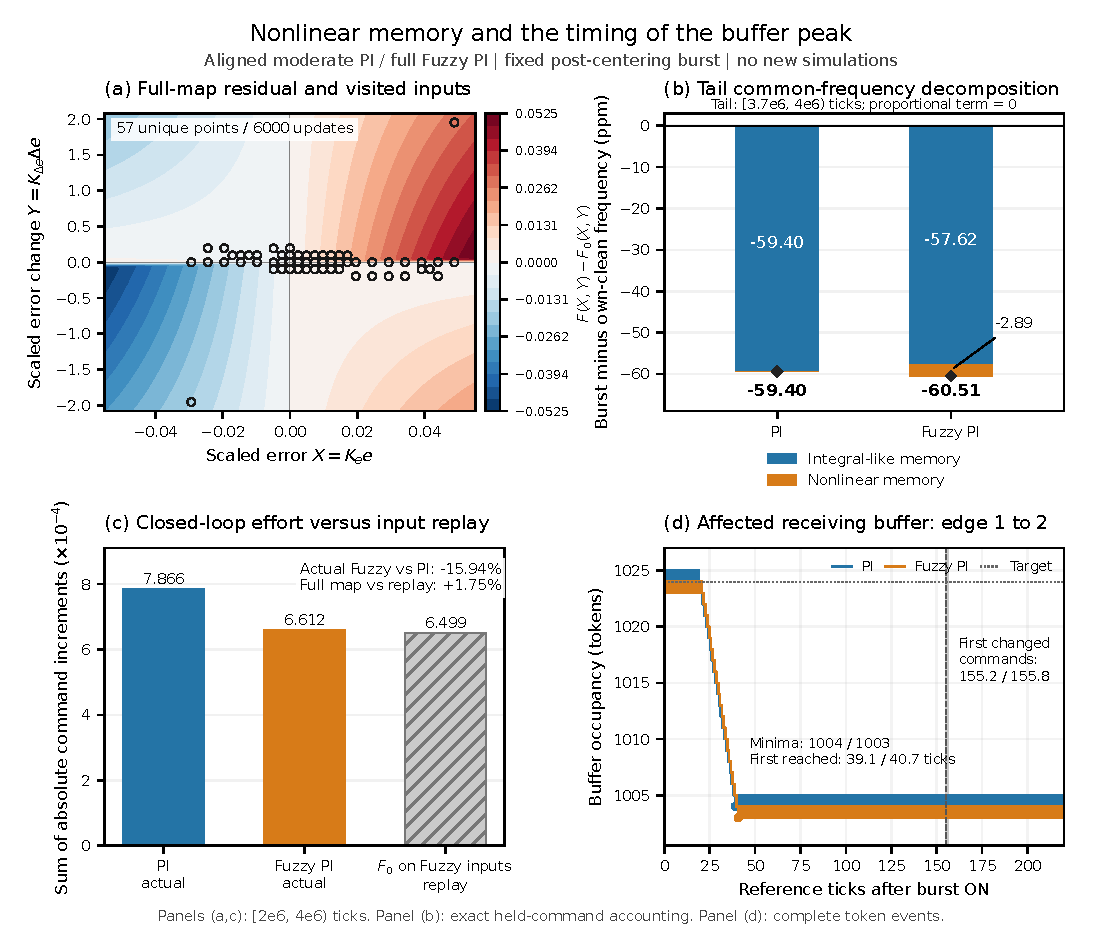
\includegraphics[width=0.97\textwidth]{images/evaluation_20261103/m2_nonlinear_memory.pdf}
% \caption{Nonlinear mechanism diagnostics reusing the four M2 runs.
% The panels show the exact central residual $F-F_0$, common-frequency
% memory accounting, command activity and complete early buffer events.
% The hatched $F_0$ activity bar is a replay on Fuzzy's measured inputs,
% not a third closed-loop experiment. The residual surface is multiplied
% by negative $K_u$ in the controller. The memory panel uses
% $[3.7\times10^6,4\times10^6)$; activity uses the main disturbance
% window. First peak attainment precedes the first changed command, but
% the peak can be revisited after feedback begins.}
% \Description{Four panels connecting Fuzzy rule residuals, stored correction
% memory, command total variation, and early buffer depletion timing.}
% \label{fig:eval_mechanism}
% \end{figure*}
% 
% \subsection{Independent paired random-latency validation}
% \label{detail:subsec:eval_random}
% 
% All 180 M3 validation runs are normal-admissible, with zero saved-state
% mismatches in complete-event replay. Table~\ref{detail:tab:eval_random}
% summarizes the primary endpoint. The ratio estimand is
% \begin{equation}
%  \widehat r=\frac1{30}\sum_{s=1}^{30}
%        \frac{R_{W,s}^{\rm Fuzzy}}{R_{W,s}^{\rm PI}},
%  \label{detail:eq:eval_paired_ratio}
% \end{equation}
% where $s$ indexes independent seeds. It is not the ratio of the two
% group means. Pointwise 95\% confidence intervals (CIs) use 20,000
% paired-seed percentile-bootstrap resamples with fixed resampling seeds.
% Time points, edges and bootstrap draws are not independent experimental
% replications. Regimes are analyzed separately; the intervals do not
% provide simultaneous multiple-endpoint coverage. There are no excluded
% pairs in the reported comparisons.
% 
% \begin{table*}[t]
% \caption{M3 primary disturbance-window disagreement RMS. Controller entries
% are means over 30 seeds in ppm. Ratios are means of paired seed ratios
% with pointwise 95\% CIs. A ratio below one favors Fuzzy.}
% \label{detail:tab:eval_random}
% \centering
% \begin{tabular}{@{}lrrrll@{}}\toprule
% Profile grid & PI moderate & PI stronger & Fuzzy & Fuzzy/moderate [CI] & Fuzzy/stronger [CI]\\\midrule
% $T_c=1000$ & 4.911 & 9.347 & 5.856 & 1.1925 [1.1722,1.2150] & 0.6266 [0.6155,0.6389]\\
% $T_c=10000$ & 6.696 & 9.699 & 7.152 & 1.0679 [1.0624,1.0736] & 0.7365 [0.7184,0.7554]\\\bottomrule
% \end{tabular}
% \end{table*}
% 
% \begin{figure*}[t]
% \centering
% 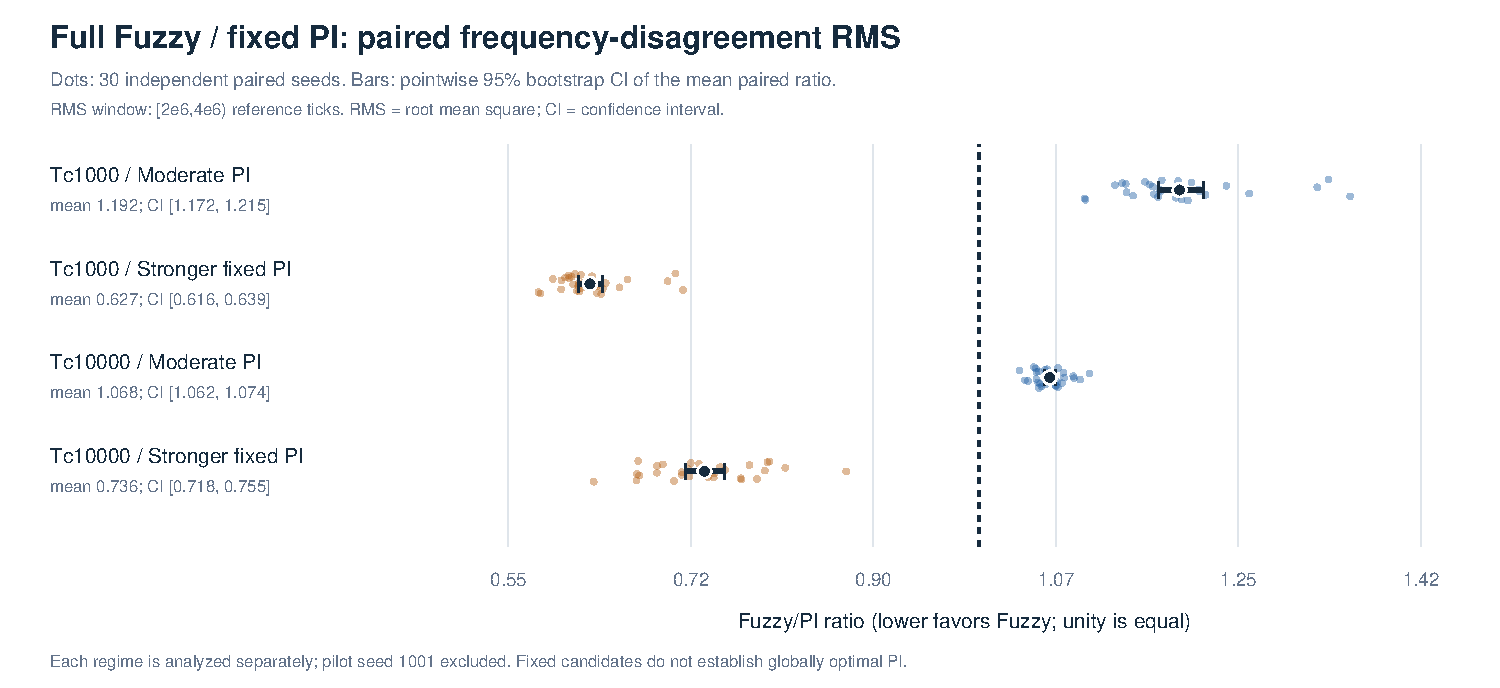
\includegraphics[width=0.97\textwidth]{images/evaluation_20261103/m3_primary_paired_effects.pdf}
% \caption{Independent paired random-latency validation: primary disagreement
% RMS and paired Fuzzy/PI effects for two physical profile grids. Thirty
% seeds per regime are shared across the three fixed controllers. The
% moderate comparator is the primary axis-matched PI baseline; stronger
% PI is a separate fixed candidate. Ratios and pointwise confidence
% intervals follow the paired-seed protocol, rather than resampling
% correlated controller updates.}
% \Description{Primary random-latency disagreement results and paired effects
% against moderate and stronger fixed PI for thirty seeds per regime.}
% \label{detail:fig:eval_random_primary}
% \end{figure*}
% 
% Relative to moderate PI, Fuzzy has higher RMS in all 30 seeds of each
% regime: mean paired increases are 19.245\% and 6.791\%. The lower
% RMS relative to stronger fixed PI is comparator-specific; moderate PI
% already has lower RMS than Fuzzy, so that comparison does not establish
% an inherent advantage of fuzzy inference over suitable PI tuning.
% The frozen random-latency hypothesis of lower disagreement RMS is
% therefore not supported against the primary baseline in these regimes.
% 
% Within the disturbance windows, all runs have at most seven frames of
% actual target deviation and at least 1017 frames of lower/upper
% headroom. These extrema exclude startup. They establish finite-run
% admissibility in this interior operating region, not a larger Fuzzy
% safe set. The random result also does not extend the M2 TV reduction:
% mean paired Fuzzy/moderate TV ratios are 1.03045 and 1.03153.
% Figure~\ref{fig:eval_random_secondary} retains buffer, effort and
% common-frequency diagnostics. Mean tail common-frequency shifts from
% each controller's pre-disturbance level are approximately
% $-156.682$ versus $-72.576$ ppm at $T_c=1000$, and $-76.540$
% versus $-67.816$ ppm at $T_c=10000$ (Fuzzy versus moderate PI).
% These finite-horizon shifts and trends are reported separately from
% relative synchronization; no absolute-frequency loop is present.
% 
% \begin{figure*}[t]
% \centering
% 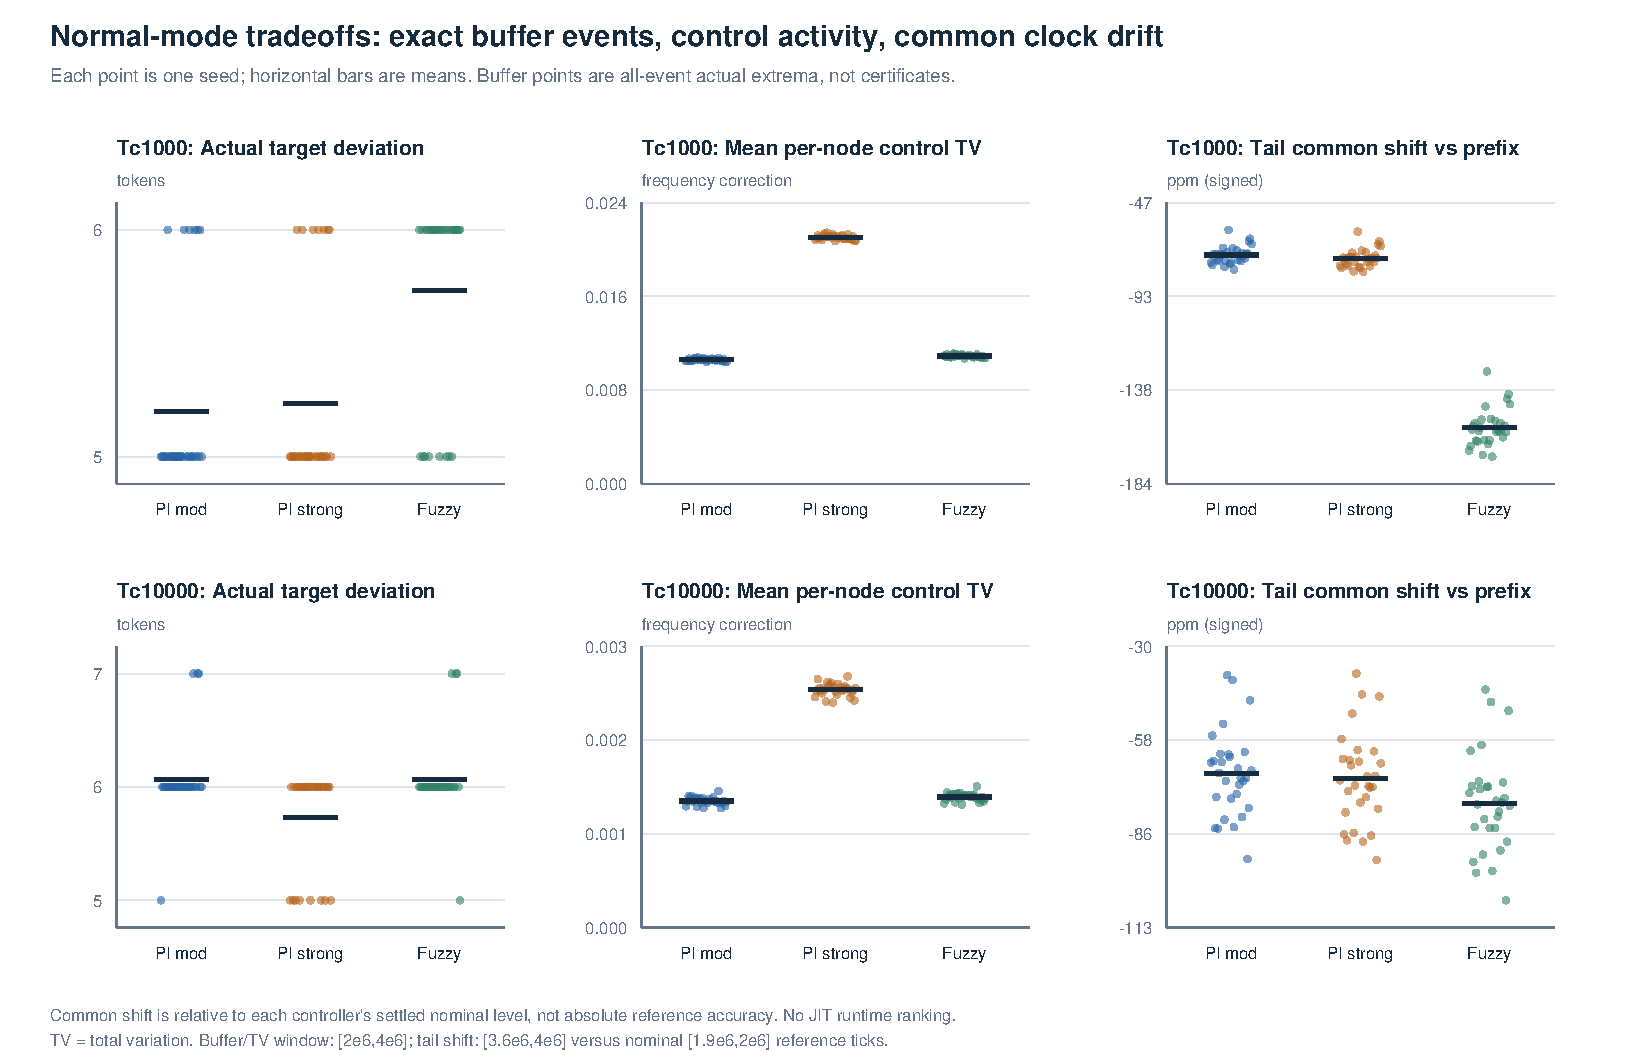
\includegraphics[width=0.97\textwidth]{images/evaluation_20261103/m3_buffer_effort_drift.pdf}
% \caption{Secondary M3 diagnostics over the declared windows: complete-event
% buffer excursions, command activity and common-frequency shift.
% The same 30 paired seeds underlie each regime; additional endpoints
% do not create additional independent replications. Buffer extrema
% refer to the disturbance window, not the startup trajectory.}
% \Description{Buffer, control activity and common-frequency diagnostics
% complementing the primary random-latency synchronization metric.}
% \label{fig:eval_random_secondary}
% \end{figure*}
% 
% \subsection{What the completed evaluation establishes}
% \label{detail:subsec:eval_support}
% 
% The evidence supports the implementation-consistent PI calibration,
% the exact nonlinear mechanism on observed M2 inputs, and the
% conditional reference-model buffer-headroom theorem. Actual Callisto
% demonstrates endpoint-dependent response shaping: a smaller full-run
% buffer excursion and lower post-burst IAE/TV at the stated M2 point,
% alongside higher post-onset peaks and no faster component recovery.
% The independent M3 study limits any general random-jitter advantage
% claim for the frozen controller. These outcomes are consistent with
% the paper's conditional mechanism-and-tradeoff formulation; they do
% not support uniform Fuzzy superiority.
% 
% The completed actual campaigns do not test the boundary of the
% reference invariant set. Their large buffer reserves cannot substitute
% for certified-safe, uncertified-but-observed-safe and failed cases
% around a common boundary. Nor do finite observations prove
% infinite-horizon safety or the reference theorem's optional
% frequency-spread tolerance in asynchronous delayed execution.
% Observed phase progress and capacity compliance support normal model
% execution; application-payload correctness and a formal refinement
% proof of logical synchrony are outside this evaluation.
% 
% Finally, these are fixed-controller comparisons, not a completed
% equal-budget tuning/held-out-test study. A separate preregistered
% tuning campaign has not completed its audit, selection and untouched
% tests; its partial results are excluded from the present performance
% tables. The evaluation also provides no P/GABA comparison, switched
% FFP or observer result, dropout recovery, serialized-link hardware
% test, or meaningful controller runtime/energy ranking. Consequently,
% practical adoption beyond the reported operating points remains an
% empirical question even though the reference-model headroom benefit
% is mathematically established.

\section{Extended Interpretation and Scope}
\label{app:discussion}
\noindent\textbf{Correspondence: Section~\ref{sec:discussion}.} This appendix preserves the extended model, intermediate steps and supporting interpretation behind the corresponding main-text section.


\label{detail:sec:discussion}

The results identify two reasons to consider the proposed Fuzzy PI law
for bittide: a provable reduction in transient buffer demand for a
specified reference execution, and independently tested synchronization
benefits in defined delivery regimes. The connection between these
results is the explicit nonlinear correction mechanism, rather than
an assumption that fuzzy inference improves every performance metric.
This section explains how the benefits should inform controller
selection and which extensions require further evidence.

\subsection{What nonlinear response shaping adds}
\label{detail:subsec:discussion_mechanism}

The controller offers a local way to change the relationship between
occupancy error, its change between measurements and the next frequency
correction. Proposition~\ref{detail:prop:fpi_central} shows that the normalized
min-activation surface strengthens its calibrated linear counterpart
for aligned input signs and attenuates its magnitude for opposing signs
within the stated central region. A uniform increase in PI gains would
scale both cases uniformly. The Fuzzy law therefore supplies
a different response shape at calibrated gain coordinates, while
retaining a concrete connection to the PI baseline implementation.

This interpretation concerns a correction increment, not a complete
closed-loop performance ordering. In particular, aligned signs do not
always mean that absolute occupancy error is increasing; an error can
cross zero while decreasing in magnitude. The plant, measurement
history and accumulated correction determine the resulting trajectory.
Equation~\eqref{detail:eq:fpd_accounting} makes the memory contribution explicit:
past nonlinear increments may remain in the accumulator even when
later inputs have zero nonlinear residual. This provides a mechanism
to investigate transient shaping and persistent offsets, but a
same-input decomposition alone does not establish their causal
contribution to differences between independently evolving closed loops.

The comparisons address two questions. The reference proof and
startup tests hold the calibrated gain coordinates fixed. They test
a prescribed change in the controller law. The
equal-budget study instead asks whether each controller family can
produce a useful selected design with the same finite search budget.
Its lower held-out RMS supports the selected Fuzzy scheme, including
its chosen gains, rather than an inference-only effect at identical
gains. Keeping these questions separate makes the empirical benefit
more meaningful than a comparison against a single arbitrary PI setting.

\subsection{Engineering meaning of the buffer-headroom benefit}
\label{detail:subsec:discussion_headroom}

For a finite receiving buffer, the largest transient deviation matters
even when the eventual operating point is admissible.
Theorem~\ref{detail:thm:btd_headroom} compares a certified upper bound for the
Fuzzy excursion with an attained PI peak, not just two conservative
upper bounds. For its prescribed initialization, the resulting
improvement in minimum headroom exceeds 6.0887 fluid frames. Both
controllers also satisfy the reference model's positive-frequency,
correction and convergence conditions. The benefit thus concerns
transient resource use while those conditions remain satisfied.

The matched-gain Callisto tests provide a separate engineering observation.
For example, at 1600 ppm, Fuzzy reduces the measured excursion from
94 to 72 frames without correction saturation or gate intervention
(Table~\ref{detail:tab:eval_startup_safety}). This is consistent with a useful
headroom effect after introducing delayed local execution and integer
buffer events, although the mathematical reference certificate does
not cover that implementation. At the larger stress scale, fewer
saturated updates and smaller excursions remain finite-run findings,
not a proof that saturation is harmless or that future overflow is
impossible.

These results measure reserve at fixed capacity. They do not establish
that a smaller hardware buffer can simply be substituted. Capacity
appears in the feedback normalization
$\gamma_i=100/(d_iC)$, where $d_i$ is the number of receiving neighbors.
Changing $C$ or the degree changes the frame-count controller map
unless the gains or normalization are adjusted consistently. Any
capacity-reduction claim would therefore require a new model-consistent
comparison and a fresh safety check. Similarly, a failed sufficient
condition is inconclusive: the observed-safe but uncertified reference cases
illustrate conservatism, not an enlarged general safe set.

\subsection{Selecting a controller for the operating regime}
\label{detail:subsec:discussion_selection}

The independent tests demonstrate a practical benefit under the stated
selection policy. With identical evaluation budgets, frozen gains and
shared held-out profiles, the random-priority Fuzzy representative
reduces disagreement RMS and mean command TV in both original random
regimes. The burst-priority representative also substantially reduces
IAE in the larger held-out burst. The distinct selected representatives
show that the desired task matters: prioritizing random disagreement
and prioritizing a burst transient need not choose the same parameters.
The experiments do not switch between these representatives online.

Several measures are needed to interpret the benefit. Relative
frequency agreement concerns differences between nodes; it does not
require the common frequency to equal one or to return to its clean
counterfactual. The larger common-frequency shift accompanying the
selected Fuzzy RMS improvement is therefore an engineering cost to
evaluate against the application, not an inconsistency in the RMS
measurement. The controller has no absolute-frequency reference loop.
Likewise, smaller buffer peaks need not coincide with the lowest RMS,
and command TV is an activity metric rather than a measured energy
cost. A design choice should specify the acceptable headroom,
frequency-shift and correction constraints before selecting among the
reported tradeoffs.

The slower-delivery study further shows why timing conditions belong
in that choice. Increasing a constant link-latency plateau does not
suspend arrivals for the whole plateau: its onset changes in-flight
inventory, and the first deficit can form before changed feedback is
applied. The ramp profiles allow regulation during the formation of
the imbalance, whereas the random profile grids change its temporal
structure. Neither a longer hold nor slower variation alone establishes
an RMS advantage. These observations motivate matching the controller
to a declared disturbance regime; they do not identify an optimal
polling period, since polling was not independently swept in the new
performance tests.

\subsection{Meaning of safety, convergence and logical synchrony}
\label{detail:subsec:discussion_scope}

The certificate applies to the synchronous zero-latency fluid model with
its compatible targets, initialization and invariant input region.
Its sampled recurrence is the exact endpoint map of that continuous
zero-order-hold reference. It is not a replacement discrete firing-count
plant, nor an exact model of the asynchronous controller scheduling
and integer delivery events in Callisto. In particular, the
complete 25-rule controller remains executable outside the central
input region, while the regional formula and the numerical invariant
certificate cannot be applied to arbitrary such trajectories.

The Callisto tests establish capacity compliance, positive frequency and
progress over specified finite records. Persistent random input is
evaluated by windowed disagreement and occupancy statistics rather
than claimed exact convergence to a fixed equilibrium. The startup
records also have a shorter declared horizon than the disturbance
tests. None of these observations alone supplies an all-time safety
or convergence proof for delayed execution. Similarly, the reference
frequency-spread result requires a separately justified engineering
threshold; logical synchrony does not supply a universal ppm limit.

Logical synchrony is the computational requirement motivating the
controller, while physical syntony, buffer centering and positive
frequency describe different properties of its implementation.
Preserving capacity and frame order, together with continued data
progress, supports the normal execution assumed here. Demonstrating
functional logical synchrony for an application would additionally
require checking the logical frame relationships and payload execution
against the corresponding logical model. These experiments do not
perform that refinement check or measure application-level useful
throughput. A capacity guard that prevents underflow by stopping data
progress must also be distinguished from successful unstalled control.

\subsection{External validity and next steps}
\label{detail:subsec:discussion_future}

The independent comparison is deliberately bounded: a three-node
triangle, a fixed two-dimensional gain grid, fixed Fuzzy input scaling
$K_e$, and one training seed per random regime. The held-out seeds
quantify variation within those declared input families; they do not
turn the search into global controller optimization or establish
performance on larger, heterogeneous or changing networks. The
transport model preserves order and permits batch release without a
finite serialization rate. Hardware oscillator limits, serialized
links, packet loss, node dropout and controller execution cost require
separate evaluation. The current observer and supervisory switching
mechanisms are disabled, so they contribute no fault-recovery claim.

The most direct theoretical extension is to account explicitly for
local sampling, bounded delay and quantization when constructing
invariant buffer and input regions. Such a result should preserve
absolute-frequency and actuator constraints as well as disagreement
bounds. Empirically, broader topologies and delivery models would
test whether the observed benefits persist beyond the present
triangle. If absolute-rate requirements or sustained saturation are
important, a common-frequency constraint or anti-windup mechanism
could be studied as a separate controller extension, followed by
fresh analysis and independent tests. These steps extend the present
mechanism and evidence without changing the scope of its proved or
measured benefits.


% Previous placeholder, preserved before the completed section was integrated.
% \section{Discussion and Limitations}
% \label{detail:sec:discussion}
% \noindent\textbf{Draft status: to be written.}
% The full discussion remains pending. The certificate in
% Section~\ref{detail:sec:btd_reference} applies to its specified synchronous,
% zero-delay fluid reference and prescribed initialization. It does not
% certify asynchronous, delayed, quantized Callisto execution or establish
% universal superiority over PI.

\endgroup

\end{document}
